\documentclass[oneside, b5paper]{book}
%% 总设置
\usepackage{xeCJK} % 中英日支持
\usepackage{fontspec}
\setCJKmainfont[
    Path=fonts/,
    UprightFont = *-Regular,
    ItalicFont = *-Italic
]{LXGWBright}
\setmainfont[
    Path=fonts/,
    UprightFont = *-Regular,
    ItalicFont = *-Italic
]{LXGWBright}
\usepackage{hyperref} % 超链接引用
\hypersetup{
    colorlinks=true,
    linkcolor=blue,
    pdftitle={EJU PHY},
    pdfauthor={PENG AO}
}
\usepackage[yyyymmdd]{datetime}
\renewcommand{\dateseparator}{-}
%% 图片与插图设置
\usepackage{graphicx} % 图片插入
\graphicspath{{./img}}
\usepackage{amsmath} % 一般公式
\usepackage{extarrows} % 上下标长符号
\usepackage[version=4]{mhchem} % 化学符号
\allowdisplaybreaks % 公式跨页
\usepackage{amssymb} % 特殊符号
\usepackage{tikz} % 2d绘图
\usepackage{tikz-3dplot} % 3d绘图
\usepackage{circuitikz} % 电路绘图
\usetikzlibrary{
    decorations.pathmorphing,
    decorations.markings,
    angles, quotes, calc
}
\tikzset{
    spring/.style={decoration={
        coil,
        segment length=1mm,
        amplitude=2mm,
        aspect=0.5,
        pre length=1.5mm,
        post length=1.5mm
    }, decorate}, % preset style for a spring
    midarrow/.style={postaction={decoration={
        markings,
        mark= at position 0.5 with {\arrow{latex}}
    }, decorate}},  % preset style for arrow inline
    xyplane/.style={canvas is xy plane at z=#1},
    xzplane/.style={canvas is xz plane at y=#1},
    yzplane/.style={canvas is yz plane at x=#1},
}
\newcommand{\drawangle}[4][$\theta$]{
    \coordinate (a) at #2;
    \coordinate (b) at #3;
    \coordinate (c) at #4;
    \draw pic [draw, "#1", angle eccentricity=1.5] {angle=a--b--c};
} % command for drawing angle
%% 文章展示设置
% 0-chapter:章节
% 1-section:小节
% 2-subsection:次小节
% 3-subsubsection:次次小节。用于实际知识点
% 4-paragraph:段落。用于次次小节内并列的小知识点,或者次小节内简短补充的知识点,一般出现在开头
% 5-subparagraph:次段落。用于段落内的并列内容
\usepackage{ascmac} % 跨页显示
\usepackage{fancybox} % 带框文本
\usepackage{multicol} % 文字分栏
\usepackage{tocloft} % 设置lof
\usepackage{indentfirst} % 段首自动缩进
\setcounter{tocdepth}{2} % 设置目录层级
\setcounter{secnumdepth}{3} % 设置小节编号层级
\renewcommand\thesubsubsection{\S} % 设置次次小节编号模式

\begin{document}
    % title + acknowledge + preface + TOC
    \frontmatter
    % title page

\begin{titlepage}
    \begin{center}
        \vspace{4cm}
        
        \rule{\textwidth}{1.2pt}
        
        \vspace{0.3cm}

        {\Huge \textbf{EJU PHY}}

        \vspace{0.3cm}

        {\LARGE A BRIEF SUMMARY}

        \vspace{0.3cm}

        {\Large \textit{version \version}}

        \rule{\textwidth}{1.2pt}

        \vspace{2cm}

        {\LARGE \textbf{PENG AO}}

        \vspace{0.5cm}
        {\Large \today}

        \vfill

        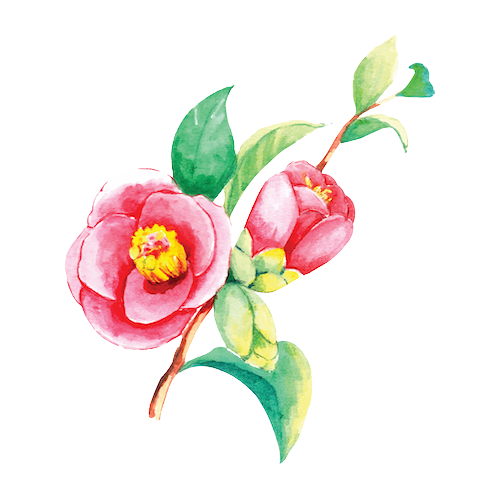
\includegraphics[width=0.382\textwidth]{automn-camellia.png}
    \end{center}
\end{titlepage}

% copyright

\clearpage
\begin{flushleft}
    \null

    \vfill
    
\includegraphics{by-nc-sa.png}

    This work is licensed under the Creative Commons Attribution-NonCommercial-ShareAlike 4.0 International License. To view a copy of this license, visit http://creativecommons.org/licenses/by-nc-sa/4.0/.

    \vspace{1em}
    You are free to:
    \begin{itemize}
        \item Share — copy and redistribute the material in any medium or format
        \item Adapt — remix, transform, and build upon the material
    \end{itemize}

    Under the following terms:
    \begin{itemize}
        \item Attribution — You must give appropriate credit, provide a link to the license, and indicate if changes were made. You may do so in any reasonable manner, but not in any way that suggests the licensor endorses you or your use.
        \item NonCommercial — You may not use the material for commercial purposes.
        \item ShareAlike — If you remix, transform, or build upon the material, you must distribute your contributions under the same license as the original.
    \end{itemize}
\end{flushleft}

% dedication

\clearpage
\begin{center}
    \null

    \vspace{0.382\textheight}
    \textit{\large
        To my gorgeous highschool life
        and meaningful university life.
    }
\end{center}

% preface

\clearpage
\chapter{前言}

\section*{自述}
本人PENG AO,来自于辽宁省沈阳市,大学本科四年级。目前就读于日本东京大学理学部情报科学科,即计算机科学专业。本文档脱胎于2019至2021年间个人授课时所整理的大纲,主要梳理了留学生统一考试理科物理的知识点,方便个人使用。

如今是2022年初春,正值本人即将迈入大学四年级之时。出于系统练习书写\LaTeX 文档,为今后学术报告、论文撰写做准备的目的,将此前的大纲进行了重新编辑。在书写过程中尽可能采取了清晰的书写结构,力争完全使用tikz绘图语言包来完成文档中的插图。

各章节内容参考了「わかりやすい高校物理の部屋」等网站和河合出版的《物理教室(四訂版)》等书籍,基于个人中学\footnote{东北育才外国语学校}时备考留学生统一考试时的所学所感加以补充。即便如此也难免有疏漏或是差错,欢迎在GitHub项目\footnote{https://github.com/PENG-AO/EJU-PHY}上开设Issue提出。

最后,对在教学过程中帮助我逐步做出优化调整的学生们以及编辑过程中辅助我校对的朋友们表示感谢。同时也希望能对有相关需求的读者起到一定的帮助作用。

\begin{center}
    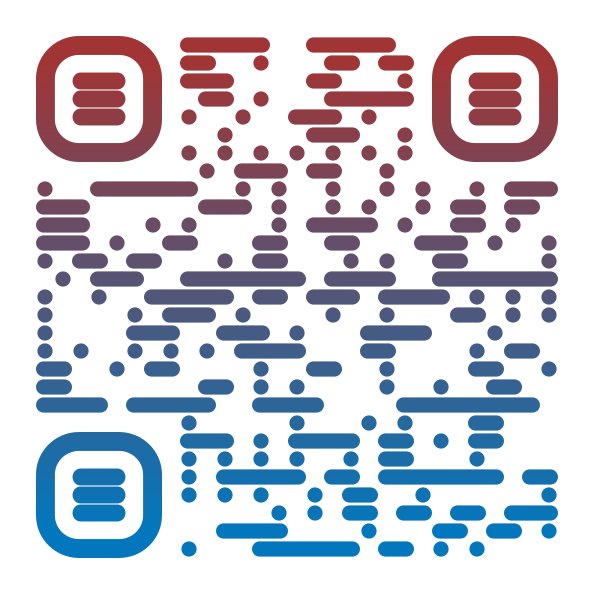
\includegraphics[width=0.16\textwidth]{repo-qrcode.png}
\end{center}

\begin{flushright}
    PENG AO\\
    2022-03-30 in Tokyo
\end{flushright}

\section*{历史}
\begin{itemize}
    \item \textit{version 1}:2019年手写版
    \item \textit{version 2}:2020年markdown电子版
    \item \textit{version 3}:2022年本文档
\end{itemize}

\section*{结构}
\begin{multicols}{2}
    \begin{itemize}
        \item 第一章:力学
        \item 第二章:热学
        \item 第三章:波动
        \item 第四章:电磁
        \item 第五章:原子
        \item 附录一:补充内容
        \item 附录二:历年考点
        \item 附录三:真题略解
        \item 附录四:配图一览
        \item 附录五:推荐书目
    \end{itemize}
\end{multicols}
本书与留学生统一考试考纲顺序相同。正文部分只保留最必要的、无法进一步割舍的考点,附录中包含了一些相关数学知识的复习、个人自娱自乐\footnote{本人非物理相关专业,仅凭兴趣基于大学通识物理的知识试做推导,难免有所谬误}的定理推导过程、和一些其他信息的汇总。读者可以通过目录中的链接自由跳转阅读。

\section*{战绩}
本人考学时参加了2018年的两次留学生统一考试,其中6月份的在香港,11月份的在日本京都。凭借如下的留学生统一考试的成绩和97分\footnote{根据当年经验,97分的成绩在绝对数值上不具备十足的优势,但尚且够用}的托福成绩得到了东京大学理学部情报科学科、京都大学工学部情报学科、名古屋大学情报学部计算机科学科和东京工业大学的录取通知书。
\begin{center}
    \renewcommand\arraystretch{1.2}
    \begin{tabular}{c|cccc|c}
        \hline
        &日语&数学2&物理&化学&\\\hline
        2018.6&372(50)&192&95&85&744\\
        2018.11&374(45)&193&95&92&754\\
        \hline
    \end{tabular}
\end{center}

% toc

\clearpage
\renewcommand{\contentsname}{目录}
\tableofcontents

    % main part
    \mainmatter
    % chapter 1

\chapter{力学}

% chapter 1 section 1

\section{运动与力}

\subsection{速度与加速度}

\subsubsection{直线运动}

\begin{figure}[ht!]
    \centering
    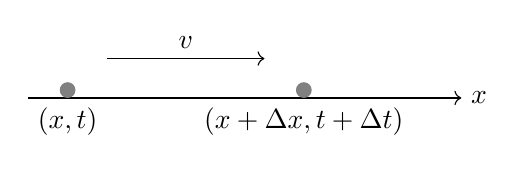
\begin{tikzpicture}
        \draw[->] (-0.5, 0) -- (5, 0) node[right] {$x$};
        \fill[fill=gray] (0, 0.1) circle (0.1);
        \node[below] at (0, 0) {$(x, t)$};
        \fill[fill=gray] (3, 0.1) circle (0.1);
        \node[below] at (3, 0) {$(x+\Delta x, t+\Delta t)$};
        \draw[->] (0.5, 0.5) -- node[above] {$v$} (2.5, 0.5);
    \end{tikzpicture}
    \caption{速度与时间}
\end{figure}

\paragraph{速度}对于在x轴上运动的物体,其在这段时间内的平均速度可如下给出:
\begin{equation*}
    \bar{v} = \frac{\Delta x}{\Delta t}
\end{equation*}
其中$\Delta x$的部分叫做変位,其方向为初始位置指向终止位置。当这个时间间隔无限趋于0时,将这个极限值称为(瞬时)速度,即:
\begin{equation*}
    v = \lim_{\Delta t\to0}\frac{\Delta x}{\Delta t}=\frac{dx}{dt}
\end{equation*}
速度的方向由变位的方向决定,单位常用$\left(m/s\right)$。其大小可以用:速度の大きさ、速さ等词汇描述。

\paragraph{加速度}与速度类似,当我们着眼于某个时间间隔内速度的变化时,便可以得到平均加速度的定义。若再将其时间间隔无限缩小至0就有了(瞬时)加速度:
\begin{equation*}
    a = \lim_{\Delta t\to0}\frac{\Delta v}{\Delta t}=\frac{dv}{dt}
\end{equation*}
同样的,由于速度是矢量所以加速度也是具有方向的,其方向取决于速度变化的方向,单位常用$\left(m/s^2\right)$。

\paragraph{图像表示}在$v-t$图像中,根据速度定义可知:
\begin{equation*}
    \textrm{变位的(微小)变化}=\textrm{速度}\times\textrm{时间的(微小)变化}
\end{equation*}
所以,数形结合可得$v-t$图像与时间轴围成的面积即为该时间间隔内物体的距离。但有些时候围成的图形会跨过时间轴,此时根据速度值的正负(方向)可分析得到:横轴以上的面积表示正方向上的距离,横轴以下的部分表示负方向上的距离。
\begin{figure}[ht!]
    \centering
    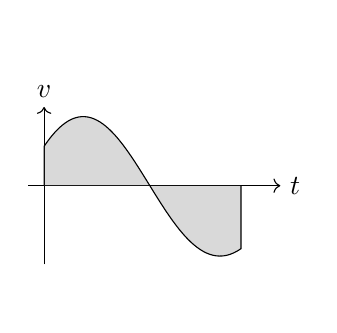
\begin{tikzpicture}
        \draw[->] (-0.2, 0) -- (3, 0) node[right] {$t$};
        \draw[->] (0, -1) -- (0, 1) node[above] {$v$};
        \filldraw[color=black, fill=gray, fill opacity=0.3] (0, 0) -- 
            (0, 0.5) .. controls (1, 2) and (1.5, -1.5) .. (2.5, -0.8) -- (2.5, 0);
    \end{tikzpicture}
    \caption{$v-t$图像}
\end{figure}
此外,根据加速度的定义,我们可以根据$v-t$图像的斜率来确定其值。
\begin{itemize}
    \item 图形面积$\implies$移动距离
    \item 切线斜率$\implies$加速度
\end{itemize}

\paragraph{等加速度直线运动}加速度一定的直线运动,属于最基本的运动类型。
\begin{figure}[ht!]
    \centering
    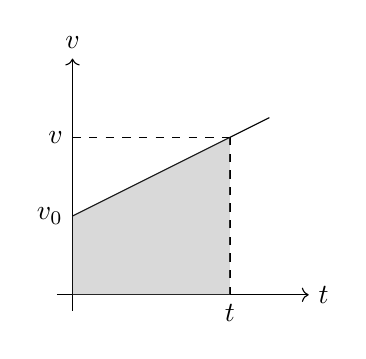
\begin{tikzpicture}
        \draw[->] (-0.2, 0) -- (3, 0) node[right] {$t$};
        \draw[->] (0, -0.2) -- (0, 3) node[above] {$v$};
        \draw[domain=0:2.5] plot (\x, {0.5*\x + 1});
        \coordinate[label=left:$v$] (v) at (0, 2);
        \coordinate[label=left:$v_0$] (v0) at (0, 1);
        \coordinate[label=below:$t$] (t) at (2, 0);
        \draw[dashed] (v) -- (2, 2);
        \draw[dashed] (t) -- (2, 2);
        \fill[fill=gray, opacity=0.3] (0, 0) -- (v0) -- (2, 2) -- (t) --cycle;
    \end{tikzpicture}
    \caption{等加速度直线运动图像}
\end{figure}

\begin{itembox}[l]{运动学基本公式}
    \begin{gather*}
        v=v_0+at\\
        x=v_0t+\frac{1}{2}at^2\\
        v^2-{v_0}^2=2ax
    \end{gather*}
\end{itembox}

\subsubsection{平面运动分析}

根据速度/加速度的矢量性,运动可以轻松地被扩展到平面上。而且倘若借助向量、坐标等数学手段,我们就可以驾驭更加复杂的运动形式。
\begin{figure}[ht!]
    \centering
    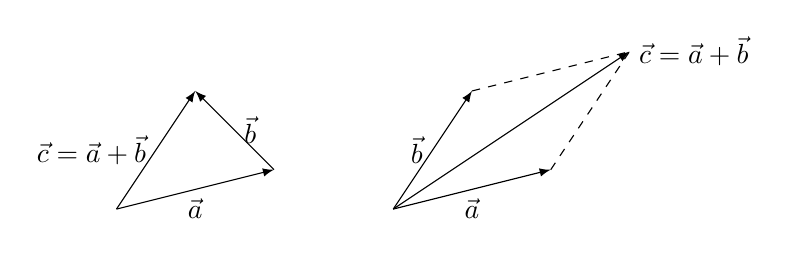
\begin{tikzpicture}
        \begin{scope}
            \draw[-latex] (0, 0) -- node[below] {$\vec{a}$} (2, 0.5);
            \draw[-latex] (2, 0.5) -- node[right] {$\vec{b}$} (1, 1.5);
            \draw[-latex] (0, 0) -- node[left] {$\vec{c}=\vec{a}+\vec{b}$} (1, 1.5);
        \end{scope}
        \begin{scope}[xshift=100pt]
            \draw[-latex] (0, 0) -- node[below] {$\vec{a}$} (2, 0.5);
            \draw[-latex] (0, 0) -- node[left] {$\vec{b}$} (1, 1.5);
            \draw[-latex] (0, 0) -- (3, 2) node[right] {$\vec{c}=\vec{a}+\vec{b}$};
            \draw[dashed] (2, 0.5) -- (3, 2);
            \draw[dashed] (1, 1.5) -- (3, 2);
        \end{scope}
    \end{tikzpicture}
    \caption{向量合成与分解}
\end{figure}
如果将上述的合成与分解放到平面直角坐标系内操作,就是最常见也最常用的形式。
\begin{figure}[ht!]
    \centering
    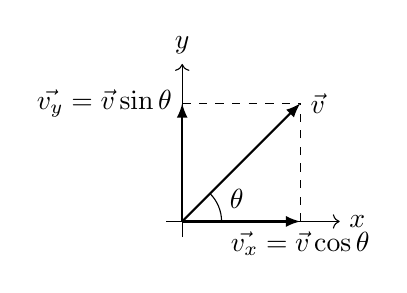
\begin{tikzpicture}
        \draw[->] (-0.2, 0) -- (2, 0) node[right] {$x$};
        \draw[->] (0, -0.2) -- (0, 2) node[above] {$y$};
        \draw[thick, -latex] (0, 0) -- (1.5, 1.5) node[right] {$\vec{v}$};
        \draw[thick, -latex] (0, 0) -- (1.5, 0) node[below] {$\vec{v_x}=\vec{v}\cos\theta$};
        \draw[thick, -latex] (0, 0) -- (0, 1.5) node[left] {$\vec{v_y}=\vec{v}\sin\theta$};
        \draw[dashed] (1.5, 0) -- (1.5, 1.5);
        \draw[dashed] (0, 1.5) -- (1.5, 1.5);
        \drawangle{(1, 0)}{(0, 0)}{(1, 1)};
    \end{tikzpicture}
    \caption{速度的正交分解}
\end{figure}
\begin{itembox}[l]{运动分析}
    \begin{itemize}
        \item 合成分解:$\vec{v}\rightleftharpoons\vec{v_1}+\vec{v_2}$
        \item 相对速度:$\textrm{相对}=\textrm{对象}-\textrm{参考/基准}$
    \end{itemize}
\end{itembox}

\subsection{运动与力}

\subsubsection{力}

力的三要素(力的大小、作用线、作用点)、单位(N)等内容比较基础,在此略过。

\paragraph{力的平衡}由于力也是矢量,所以我们也可以对其进行合成/分解的操作。一般称合成得来的力为合力,称分解得来的力为分力。在考虑受力平衡时便借助此思想,将某物体视为质点\footnote{忽略极小或质量分布均匀的物体的大小,将其视作一个点。},其合力为0的状态定义为平衡状态。个人常用$\sum\vec F=0$的方式来简记。

\paragraph{重力}吸引地表所有物体,竖直向下的力。其成因是万有引力。数学形式为:$G=m\cdot g$。

\paragraph{张力/拉力}一般指绳子上的张力或拉力。对于轻质绳子,\underline{同一条绳子}上的拉力处处相等

\paragraph{弹力}日文为弾性力,指的是弹簧为了恢复到\underline{自然长/原长}而产生的力。弹力遵循胡克定律,日文为フックの法則。使用时应注意形变量具有方向。
\begin{itembox}[l]{胡克定律}
    \begin{equation*}
        \vec{F}=-k\vec{\Delta x}\quad(k:\textrm{バネ定数},\Delta x:\textrm{基于原长的形变量})
    \end{equation*}
\end{itembox}
\begin{figure}[ht!]
    \centering
    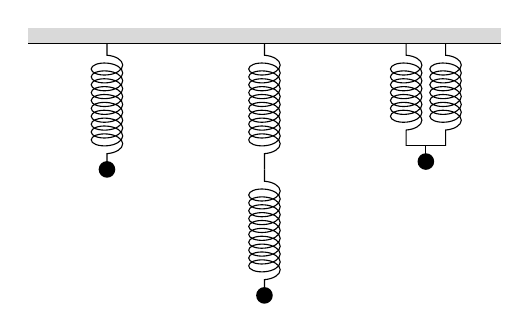
\begin{tikzpicture}
        \fill[fill=gray, opacity=0.3] (0, 0.2) rectangle (6, 0);
        \draw (0, 0) -- (6, 0); 
        \draw[spring] (1, 0) -- ++ (0, -1.6);
        \fill[fill=black] (1, -1.6) circle (3pt);
        \draw[spring] (3, 0) -- ++ (0, -1.6);
        \draw[spring] (3, -1.6) -- ++ (0, -1.6);
        \fill[fill=black] (3, -3.2) circle (3pt);
        \draw[spring] (4.8, 0) -- ++ (0, -1.3);
        \draw[spring] (5.3, 0) -- ++ (0, -1.3);
        \draw (4.8, -1.3) -- (5.3, -1.3);
        \draw (5.05, -1.3) -- (5.05, -1.5);
        \fill[fill=black] (5.05, -1.5) circle (3pt);
    \end{tikzpicture}
    \caption{弹簧串并联}
\end{figure}
\begin{itembox}[l]{弹簧串并联}
    \begin{itemize}
        \item 串联(受力一致)
        \begin{equation*}
            \begin{cases}
                F=k_1x_1=k_2x_2\\
                F=K(x_1+x_2)
            \end{cases}\implies\frac1K=\frac1{k_1}+\frac1{k_2}
        \end{equation*}
        \item 并联(形变一致)
        \begin{equation*}
            \begin{cases}
                F=F_1+F_2=k_1x+k_2x\\F=Kx
            \end{cases}\implies K=k_1+k_2
        \end{equation*}
    \end{itemize}
\end{itembox}

\paragraph{摩擦力}摩擦力来自于物体和接触面之间的支持力,日文为垂直抗力。应明确接触为要因,有接触则会产生支持力,进而才涉及摩擦力问题。其数学形式为:$f=N\cdot\mu$,其中$\mu$为摩擦系数。
\begin{figure}[ht!]
    \centering
    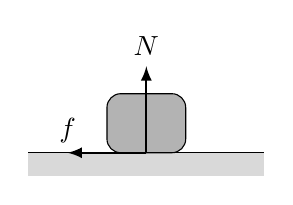
\begin{tikzpicture}
        \draw (0, 0) -- (3, 0);
        \fill[fill=gray, opacity=0.3] (0, 0) rectangle (3, -0.3);
        \filldraw[color=black, fill=gray, fill opacity=0.6, rounded corners=5pt] (1, 0) rectangle (2, 0.75);
        \draw[-latex, thick] (1.5, 0) -- (1.5, 1.1) node[above] {$N$};
        \draw[-latex, thick] (1.5, 0) -- (0.5, 0) node[above] {$f$};
    \end{tikzpicture}
    \caption{摩擦力}
\end{figure}
如果给一个物体施加一个线性变大的力,作用在其身上的摩擦力变化如图。
\begin{figure}[ht!]
    \centering
    \begin{tikzpicture}
        \draw[->] (-0.2, 0) -- (3, 0) node[right] {$t$};
        \draw[->] (0, -0.2) -- (0, 3) node[above] {$f$};
        \draw[thick] (0, 0) -- (1, 2) node[above, fill=white]{$f_0=N\cdot\mu\quad(\mu:\textrm{静止摩擦系数})$};
        \draw[thick] (1, 2) -- (1, 1.5);
        \draw[thick] (1, 1.5) -- (3, 1.5) node[right] {$f=N\cdot\mu^\prime\quad(\mu^\prime:\textrm{滑动摩擦系数})$};
    \end{tikzpicture}
    \caption{摩擦力变化}
\end{figure}
由此可知,静止摩擦力是物体在发生运动之前用来平衡外力的力,其最大值是最大静摩擦力。

\subsubsection{运动法则}

\begin{itembox}[l]{牛顿运动定律}
    \begin{itemize}
        \item 惯性法则:物体\underline{不受力}或\underline{合外力为0}时,运动状态不发生改变(惯性)。
        \item 运动法则:物体受力后会产生与力\underline{同方向}的加速度。加速度大小与力的大小成正比,与物体质量成反比。
        \begin{equation*}
            \vec{a}=k\cdot\frac{\vec{F}}{m}\to
            \vec{F}=m\vec{a}
        \end{equation*}
        \item 作用力与反作用力法则:物体A向物体B施力后,会受到来自物体B的\underline{大小相等}、\underline{方向相反}(等大反向)的力。
    \end{itemize}
\end{itembox}
其中惯性法则揭示的本质问题是:力是改变物体运动状态的原因。同时应注意,作用力与反作用力的分析对象为两个物体,而受力平衡则只针对单个物体论。

\subsubsection{重力相关的运动}

\paragraph{落体运动}根据物体的初速度有以下三种情况。
\begin{itemize}
    \item 自由落体:初速度为0,只受重力。
    \item 上抛运动:初速度向上为$v_0$,只受重力。
    \item 下抛运动:初速度向下为$v_0$,只受重力。
\end{itemize}
将上述条件代入运动学基本公式就可得该特殊情形下的运动方程。
\begin{itembox}[l]{自由落体}
    \begin{equation*}
        \begin{cases}
            v=gt\\
            h=\frac{1}{2}gt^2\\
            v^2=2gh
        \end{cases}
    \end{equation*}
\end{itembox}

\paragraph{抛体运动}将落体运动扩展到平面内得到的便是抛体运动。
\begin{figure}[ht!]
    \centering
    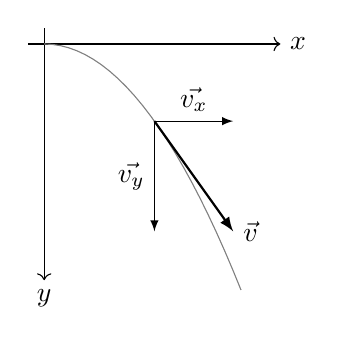
\begin{tikzpicture}
        \draw[->] (-0.2, 0) -- (3, 0) node[right] {$x$};
        \draw[->] (0, 0.2) -- (0, -3) node[below] {$y$};
        \draw[color=gray, domain=0:2.5] plot (\x, {-0.5*\x^2});
        \draw[thick, -latex] (1.4, -0.98) -- (2.4, -2.38) node[right] {$\vec{v}$};
        \draw[-latex] (1.4, -0.98) -- node[above] {$\vec{v_x}$} (2.4, -0.98);
        \draw[-latex] (1.4, -0.98) -- node[left] {$\vec{v_y}$} (1.4, -2.38);
    \end{tikzpicture}
    \caption{平抛运动}
\end{figure}
\subparagraph{平抛运动}
\begin{itemize}
    \item 条件:水平初速度为$v_0$,只受重力。
    \item 分析:
    \begin{equation*}
        \begin{cases}
            \textrm{水平}:a_x=0\implies\textrm{匀速直线运动}\\
            \textrm{竖直}:a_y=g\implies\textrm{自由落体}
        \end{cases}
    \end{equation*}
\end{itemize}

\begin{figure}[ht!]
    \centering
    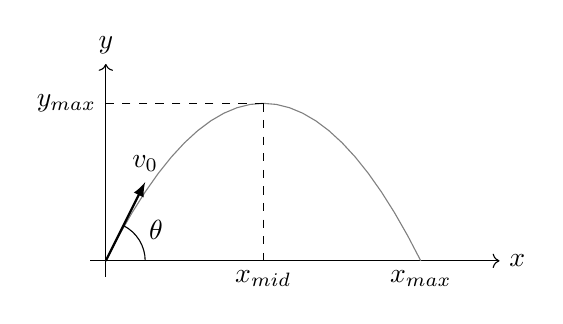
\begin{tikzpicture}
        \draw[->] (-0.2, 0) -- (5, 0) node[right] {$x$};
        \draw[->] (0, -0.2) -- (0, 2.5) node[above] {$y$};
        \draw[color=gray, domain=0:4] plot (\x, {-0.5*(\x-2)^2+2});
        \draw[thick, -latex] (0, 0) -- (0.5, 1) node[above] {$v_0$};
        \drawangle{(1, 0)}{(0, 0)}{(1, 2)};
        \draw[dashed] (2, 2) -- (2, 0) node[below] {$x_{mid}$};
        \draw[dashed] (2, 2) -- (0, 2) node[left] {$y_{max}$};
        \node[below] at (4, 0) {$x_{max}$};
    \end{tikzpicture}
    \caption{斜抛运动}
\end{figure}
\subparagraph{斜抛运动}
\begin{itemize}
    \item 条件:初速度为$v_0$,倾角$\theta$,只受重力。
    \item 分析:
    \begin{equation*}
        \begin{cases}
            \textrm{水平:初速度}v_0\cos\theta,\textrm{不受力}\implies\textrm{匀速直线运动}\\
            \textrm{竖直:初速度}v_0\sin\theta,\textrm{受重力}\implies\textrm{上抛运动}
        \end{cases}
    \end{equation*}
    \item 结论1:纵向最大高度
    \begin{gather*}
        \begin{cases}
            v=v_0\sin\theta-gt\\
            y=v_0\sin\theta t-\frac{1}{2}gt^2
        \end{cases}\\
        v=0,\textrm{即}t=\frac{v_0\sin{\theta}}{g}\textrm{时}
        y=\frac{{v_0}^2\sin^2{\theta}}{2g}\textrm{最高}
    \end{gather*}
    \item 结论2:滞空时间
    \begin{equation*}
        y=0\implies t=0,\frac{2v_0\sin{\theta}}{g}\textrm{(对称)}
    \end{equation*}
    \item 结论3:最远距离
    \begin{gather*}
        x=v_0\cos{\theta}\frac{2v_0\sin\theta}{g}=\frac{{v_0}^2\sin{2\theta}}{g}\\
        \therefore\theta=45^\circ\textrm{时},x=\frac{{v_0}^2}{g}\textrm{最大}
        \end{gather*}
\end{itemize}

\subsection{刚体与力}

\subsubsection{刚体}

与质点类似,刚体也是为分析方便而引入的一种理想模型。对于一般物体来说当受力时不可避免地会产生些许形变,然而处理大多数问题的过程中,这些形变无关紧要。那么,不考虑受力形变的刚体便应运而生。

\subsubsection{力矩}

日文为力のモーメント,是一种描述物体绕轴旋转情况的物理量。标准定义为力臂(腕の長さ)和力的向量积\footnote{力矩:$\vec{M}=\vec{r}\times\vec{F}$}。因此力矩是一个矢量,由旋转方向和旋转的强度构成,但解题时常常将这两个信息分开考虑。
\begin{figure}[ht!]
    \centering
    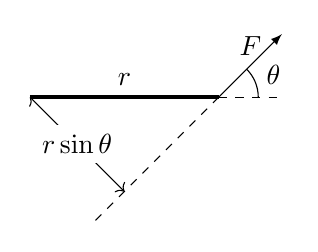
\begin{tikzpicture}[scale=0.8]
        \draw[ultra thick] (0, 0) -- node[above] {$r$} (3, 0);
        \draw[-latex] (3, 0) -- node[above] {$F$} (4, 1);
        \draw[dashed] (3, 0) -- (4, 0);
        \drawangle{(4, 0)}{(3, 0)}{(4, 1)};
        \draw[dashed] (3, 0) -- (1, -2);
        \draw[<->] (0, 0) -- node[fill=white] {$r\sin\theta$} (1.5, -1.5);
    \end{tikzpicture}
    \caption{力矩}
\end{figure}
\begin{itembox}[l]{力矩}
    \begin{equation*}
        M=F\cdot r\cdot\sin\theta
    \end{equation*}
\end{itembox}

\subsubsection{非共点力刚体平衡}

在考虑刚体平衡时,除了需要满足牛顿第一定律的条件以外,还需要保证物体自身不能旋转,即力矩平衡。
\begin{itembox}[l]{刚体平衡条件}
    \begin{itemize}
        \item 受力平衡:$\sum\vec{F}=0$
        \item 力矩平衡:$\sum\vec{M}=0$
    \end{itemize}
\end{itembox}
因此,在刚体上做力的合成时需要确保其总力矩不发生改变。

% chapter 1 section 2

\section{能量与动量}

\subsection{能量}
\label{subsec:能量}

\subsubsection{功与功率}

倘若物体在力F的作用下运动了s距离,则说该力对物体做了功,日文为仕事,其单位是$J=N\cdot m$。即功是\underline{力在运动方向上随距离的累积}。其严格定义是力与位移的标量积。
\begin{figure}[ht!]
    \centering
    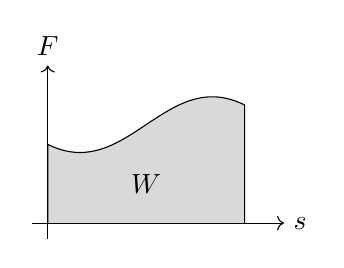
\begin{tikzpicture}
        \draw[->] (-0.2, 0) -- (3, 0) node[right] {$s$};
        \draw[->] (0, -0.2) -- (0, 2) node[above] {$F$};
        \filldraw[color=black, fill=gray, fill opacity=0.3] (0, 0) -- 
            (0, 1) .. controls (1, 0.5) and (1.5, 2) .. (2.5, 1.5) -- (2.5, 0);
        \node at (1.25, 0.5) {$W$};
    \end{tikzpicture}
    \caption{$F-s$图像与功}
\end{figure}
如果物体能对外做功,便说该物体具有能量。
\begin{itembox}[l]{功}
    \begin{equation*}
        W=\vec{F}\cdot\vec{s}=Fs\cos\theta
    \end{equation*}
    \begin{itemize}
        \item 可正可负,取决于位移的方向
        \item 力与位移方向垂直时不做功,$W=0$
    \end{itemize}
\end{itembox}
此外,类比于距离与速度的关系,单位时间内所做的功称为功率,日文为仕事率,其单位是$W=J/s$。处理问题时除了定义式,也常用$P=\frac{W}{t}=\frac{\vec{F}\cdot\vec{s}}{t}=\vec{F}\cdot\vec{v}$。

\subsubsection{动能}

日文为運動エネルギー,专指\underline{运动中}的物体具有的能量。
\begin{itembox}[l]{动能}
    \begin{equation*}
        E_k=\frac12mv^2
    \end{equation*}
\end{itembox}
如图所示,在光滑水平面上,质量为m的物体受恒力F作用运动了s距离。
\begin{figure}[ht!]
    \centering
    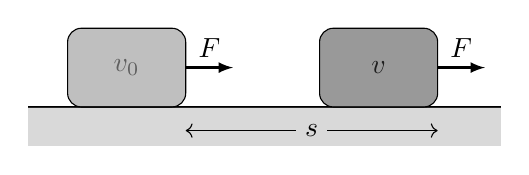
\begin{tikzpicture}
        \draw (0, 0) -- (6, 0);
        \fill[fill=gray, opacity=0.3] (0, 0) rectangle (6, -0.5);
        \filldraw[color=black, fill=gray, fill opacity=0.5, rounded corners=5pt] (0.5, 0) rectangle node {$v_0$} (2, 1);
        \draw[thick, -latex] (2, 0.5) -- node[above] {$F$} (2.6, 0.5);
        \filldraw[color=black, fill=gray, fill opacity=0.8, rounded corners=5pt] (3.7, 0) rectangle node {$v$} (5.2, 1);
        \draw[thick, -latex] (5.2, 0.5) -- node[above] {$F$} (5.8, 0.5);
        \draw[<->] (2, -0.3) -- node[fill=gray!30] {$s$} (5.2, -0.3);
    \end{tikzpicture}
    \caption{动能定理}
\end{figure}
在此期间速度从$v_0$变化为了$v$。由牛二定律和运动学基本公式可得
\begin{equation*}
    W_{\textrm{外}}=Fs=mas=\frac12m(v^2-{v_0}^2)=\Delta E_k
\end{equation*}
即在这个过程中外力做功转化为了物体动能的增量。

\subsubsection{势能}

potential energy,日文为位置エネルギー。从英日双语着眼则可对“势”一字简做解析:势能这种能量是潜在的,并且是由物体\underline{位置状态}的改变激发。其具体定义为:物体从当前位置回到基准位置时保存力\footnote{做功与路径无关的力:重力、弹簧弹力、万有引力、电场力等}所做的功。

\begin{itembox}[l]{势能}
    \begin{itemize}
        \item 重力势能(重力による位置エネルギー):
        \begin{equation*}
            E_p=mgh
        \end{equation*}
        \item 弹力势能(弾性力による位置エネルギー):
        \begin{equation*}
            E_p=\frac12kx^2
        \end{equation*}    
    \end{itemize}
\end{itembox}

\subsubsection{机械能}

日文为力学的エネルギー,是动能与势能的统称,
\begin{itembox}[l]{机械能}
    \centering
    力学的エネルギー=運動エネルギー+位置エネルギー
\end{itembox}
在只有保存力做功或者非保存力不做功的情况下守恒。更一般的,因为系统内能量的总和始终一定,只是做了形式上的转化,所以对于非保存力参与的一般情况,可以采取如下两种思路处理问题。

\begin{itemize}
    \item 仅保存力参与:初始时总能量=终止时总能量
    \item 非保存力参与:终始总能量差额=消耗的能量
\end{itemize}

\subsection{动量}
\label{subsec:动量}

\subsubsection{动量与冲量}

\begin{figure}[ht!]
    \centering
    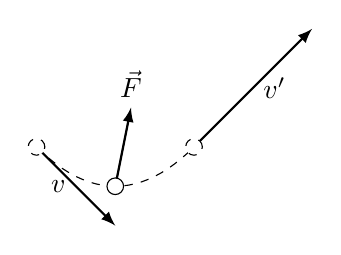
\begin{tikzpicture}
        \draw[dashed, domain=0:2] plot (\x, {0.5*(\x-1)^2-0.5});
        \draw[thick, -latex] (0, 0) -- node[left] {$v$} (1, -1);
        \draw[dashed, fill=white] (0, 0) circle (3pt);
        \draw[thick, -latex] (2, 0) -- node[right] {$v^\prime$} (3.5, 1.5);
        \draw[dashed, fill=white] (2, 0) circle (3pt);
        \draw[thick, -latex] (1, -0.5) -- (1.2, 0.5) node[above] {$\vec{F}$};
        \draw[fill=white] (1, -0.5) circle (3pt);
    \end{tikzpicture}
    \caption{动量与冲量}
\end{figure}
如图,对于质量为m的物体,在极短的时间t内施加一个力F,使其速度从$v$变为了$v^\prime$,观察其运动方程可知
\begin{gather*}
    \vec{F}=m\vec{a}=m\frac{\vec{v^\prime}-\vec{v}}{\Delta t}\\
    \vec{F}\Delta t=m\vec{v^\prime}-m\vec{v}
\end{gather*}
称其中$\vec{F}\Delta t$的部分为冲量,日文为力積,$m\vec{v}$的部分为动量,日文为運動量。由此可见,动量变化等于冲量\footnote{类比于功,可以说冲量是力在运动方向上随时间的累积}。

\subsubsection{动量守恒}

\begin{figure}[ht!]
    \centering
    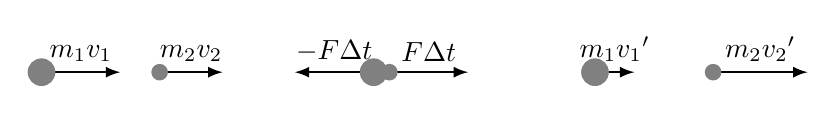
\begin{tikzpicture}
        \begin{scope}[xshift=-120]
            \draw[thick, -latex] (0, 0) -- node[above] {$m_1v_1$} ++ (1, 0);
            \fill[color=gray] (0, 0) circle (5pt);
            \draw[thick, -latex] (1.5, 0) -- node[above] {$m_2v_2$} ++ (0.8, 0);
            \fill[color=gray] (1.5, 0) circle (3pt);
        \end{scope}
        \begin{scope}
            \draw[thick, -latex] (0, 0) -- node[above] {$-F\Delta t$} ++ (-1, 0);
            \fill[color=gray] (0, 0) circle (5pt);
            \draw[thick, -latex] (0.2, 0) -- node[above] {$F\Delta t$} ++ (1, 0);
            \fill[color=gray] (0.2, 0) circle (3pt);
        \end{scope}
        \begin{scope}[xshift=80]
            \draw[thick, -latex] (0, 0) -- node[above] {$m_1{v_1}^\prime$} ++ (0.5, 0);
            \fill[color=gray] (0, 0) circle (5pt);
            \draw[thick, -latex] (1.5, 0) -- node[above] {$m_2{v_2}^\prime$} ++ (1.2, 0);
            \fill[color=gray] (1.5, 0) circle (3pt);
        \end{scope}
    \end{tikzpicture}
    \caption{动量守恒}
\end{figure}
对于上图的情形,根据牛三定律可得如下联立式:
\begin{equation*}
    \begin{cases}
        \vec{F}\cdot\Delta t&=m_2\vec{{v_2}^\prime}-m_2\vec{v_2}\\
        -\vec{F}\cdot\Delta t&=m_1\vec{{v_1}^\prime}-m_1\vec{v_1}
    \end{cases}
\end{equation*}
两侧相加整理后可得如下结论。
\begin{itembox}[l]{动量守恒}
    \begin{equation*}
        m_1\vec{v_1}+m_2\vec{v_2}=m_1\vec{{v_1}^\prime}+m_2\vec{{v_2}^\prime}
    \end{equation*}
\end{itembox}
其中左侧为碰撞前两物体的总动量,右侧为碰撞后两物体的总动量,因此在上述情形下动量守恒。

一般的,在由任意个物体组成的系统内,只要不受外力就都会满足动量守恒。而且根据动量的矢量性,其守恒也不局限于直线上,也可扩展到空间内。此时,即便有某一方向不满足条件,我们仍然可以列满足那个方向上的动量守恒。常见模型除了碰撞以外还有单个物体的分裂等。

\subsubsection{反弹系数}

日文为反発係数或者はねかえり係数,是一个描述两物体碰撞效果的数值。
\begin{itembox}[l]{反弹系数}
    \begin{equation*}
        e=-\frac{{v_1}^\prime-{v_2}^\prime}{v_1-v_2}\quad(0\le e\le1)
    \end{equation*}
    \begin{itemize}
        \item $e=0$:完全非弹性碰撞
        \item $0<e<1$:非弹性碰撞
        \item $e=1$:弹性碰撞(此时动能守恒)
    \end{itemize}
\end{itembox}
结合动量守恒公式可得两物体碰撞后速度的一般公式。
\begin{itembox}[l]{一般碰撞公式}
    \begin{equation*}
        \begin{cases}
            {v_1}^\prime=\frac{1}{m_1+m_2}(m_1v_1+m_2v_2-em_2(v_1-v_2))\\
            {v_2}^\prime=\frac{1}{m_1+m_2}(m_1v_1+m_2v_2+em_1(v_1-v_2))
        \end{cases}
    \end{equation*}
\end{itembox}

\subsubsection{特殊实例}

\paragraph{一动碰一静}即$v_2=0$的一般碰撞。此时一般碰撞公式会有所简化,而且两物体碰撞问题以此题型居多。
\begin{itembox}[l]{简化碰撞公式}
    \begin{equation*}
        \begin{cases}
            v_1=\frac{1}{m_1+m_2}(m_1-em_2)v\\
            v_2=\frac{1}{m_1+m_2}(m_1+em_1)v
		\end{cases}
    \end{equation*}
\end{itembox}

\paragraph{固定面碰撞}物体与墙面、地面等固定面碰撞的问题,其速度变化、高度变化十分具有代表性。
\begin{figure}[ht!]
    \centering
    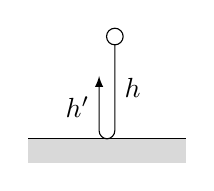
\begin{tikzpicture}
        \draw (0, 0) -- (2, 0);
        \fill[fill=gray, opacity=0.3] (0, 0) rectangle (2, -0.3);
        \draw[-latex, rounded corners=3pt] (1.1, 1.3) -- node[right] {$h$} (1.1, 0) -- (0.9, 0) -- node[left] {$h^\prime$} (0.9, 0.8);
        \draw[fill=white] (1.1, 1.3) circle (3pt);
    \end{tikzpicture}
    \caption{固定面碰撞}
\end{figure}
\begin{itembox}[l]{固定面碰撞结论}
    \begin{equation*}
        \begin{cases}
            v^\prime=ev\\
            h^\prime=e^2h
        \end{cases}
    \end{equation*}
\end{itembox}

\paragraph{斜向碰撞} 倘若物体从斜方向而来与平面发生碰撞,则需要利用运动的矢量性,将其分解处理。
\begin{figure}[ht!]
    \centering
    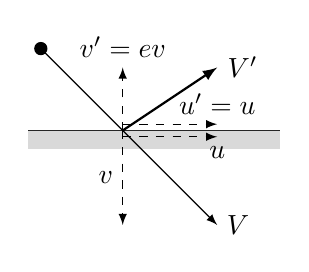
\begin{tikzpicture}[scale=0.8]
        \draw (0, 0) -- (4, 0);
        \fill[fill=gray, opacity=0.3] (0, 0) rectangle (4, -0.3);
        \fill (0.2, 1.3) circle (3pt);
        \draw[-latex] (0.2, 1.3) -- (3, -1.5) node[right] {$V$};
        \draw[dashed, -latex] (1.5, 0) -- node[left] {$v$} (1.5, -1.5);
        \draw[dashed, -latex] (1.5, -0.1) -- (3, -0.1) node[right, below] {$u$};
        \draw[dashed, -latex] (1.5, 0) -- (1.5, 1) node[above] {$v^\prime=ev$};
        \draw[dashed, -latex] (1.5, 0.1) -- (3, 0.1) node[right, above] {$u^\prime=u$};
        \draw[thick, -latex] (1.5, 0) -- (3, 1) node[right] {$V^\prime$};
    \end{tikzpicture}
    \caption{斜向碰撞}
\end{figure}

% chapter 1 section 3

\section{特殊运动}

\paragraph{惯性力}为非惯性系\footnote{系统参照物做非等速直线运动的系}下维持平衡的力,在部分情形下会使问题分析变得简单。
\begin{figure}[ht!]
    \centering
    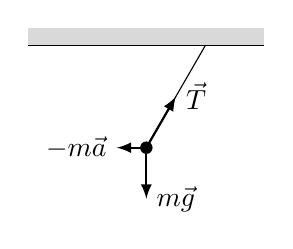
\begin{tikzpicture}[scale=0.75]
        \draw (-1, 0) -- (3, 0);
        \fill[fill=gray, opacity=0.3] (-1, 0) rectangle (3, 0.3);
        \draw (2, 0) -- (1, {-sqrt(3)});
        \fill (1, {-sqrt(3)}) circle (3pt);
        \draw[thick, -latex] (1, {-sqrt(3)}) -- ++ (-0.5, 0) node[left] {$-m\vec{a}$};
        \draw[thick, -latex] (1, {-sqrt(3)}) -- ++ (0.5, {0.5*sqrt(3)}) node[right] {$\vec{T}$};
        \draw[thick, -latex] (1, {-sqrt(3)}) -- ++ (0, {-0.5*sqrt(3)}) node[right] {$m\vec{g}$};
    \end{tikzpicture}
    \caption{非惯性系}
\end{figure}

\subsection{圆周运动}

\subsubsection{等速圆周运动}

\begin{figure}[ht!]
    \centering
    \begin{minipage}[t]{0.48\textwidth}
        \centering
        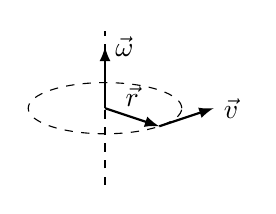
\begin{tikzpicture}[scale=0.65]
            \draw[dashed] (0, -1.5) -- (0, 1.5);
            \draw[thick, -latex] (0, 0) -- (0, 1.2) node[right] {$\vec{\omega}$};
            \draw[dashed] (0,0) circle (1.5 and 0.5);
            \draw[thick, -latex] (0, 0) -- node[above] {$\vec{r}$} (-45:1.5 and 0.5);
            \draw[thick, -latex] (-45:1.5 and 0.5) -- ++ (45:1.5 and 0.5) node[right] {$\vec{v}$};
        \end{tikzpicture}
        \caption{角速度}
    \end{minipage}
    \begin{minipage}[t]{0.48\textwidth}
        \centering
        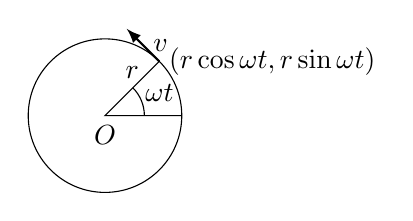
\begin{tikzpicture}[scale=0.65]
            \draw (0, 0) circle (1.5) node[below] {$O$};
            \draw (1.5, 0) -- (0, 0) -- node[above] {$r$} (45:1.5) node[right] {$(r\cos\omega t, r\sin\omega t)$};
            \drawangle[$\omega t$]{(1, 0)}{(0, 0)}{(45:1)};
            \draw[thick, -latex] (45:1.5) -- node[right] {$v$} ++ ($0.6*(135:1.5)$);
        \end{tikzpicture}
        \caption{圆周运动加速度}
    \end{minipage}
\end{figure}
\begin{itembox}[l]{角速度与周期}
    \begin{equation*}
        \omega = \frac{d\theta}{dt}
    \end{equation*}
    \begin{itemize}
        \item 单位:$rad/s$
        \item 线速度:$v=\omega r$
        \item 周期:$T=\frac{2\pi}{\omega}$
    \end{itemize}
\end{itembox}
作为对圆周运动方式的本质描述,角速度是同时具有方向与大小的矢量,其标准定义为:$\vec{\omega}=\frac1{r^2}\vec{r}\times\vec{v}$。
\begin{itembox}[l]{圆周运动加速度}
    \begin{itemize}
        \item 大小:
        \begin{equation*}
            a=\omega^2r=\frac{v^2}{r}
        \end{equation*}
        \item 方向:指向圆心
    \end{itemize}
\end{itembox}

\paragraph{向心力}物体做圆周运动的过程中时时刻刻都在改变着运动状态,那么实现这个改变的力便是\underline{向心力}。同时在生活中也常常使用离心力一词,在物理中也同样存在这个说法,其与向心力的区别在于观察角度的不同。
\begin{itemize}
    \item 向心力:是惯性系下观察时维持圆周运动的合外力
    \item 离心力:日文为遠心力,是非惯性系下观察时是物体保持静止的力
\end{itemize}
事实上,解决圆周问题的核心就在于发现是什么力构成了向心力。

\paragraph{圆锥摆}日文为円すい振り子,是一种简单常见的平面圆周运动模型。
\begin{figure}[ht!]
    \centering
    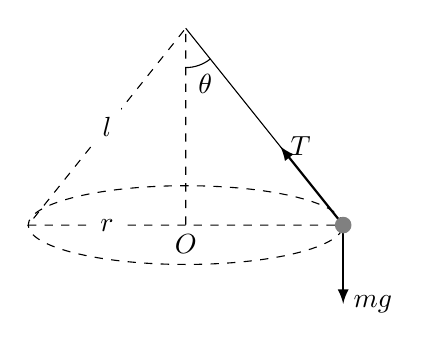
\begin{tikzpicture}
        \begin{scope}[yscale=0.25]
            \draw[dashed] (0, 0) circle (2);
        \end{scope}
        \draw[dashed] (0, 0) -- node[fill=white] {$r$} (-2, 0) -- node[fill=white] {$l$} (0, 2.5) -- (0, 0) node[below] {$O$} -- (2, 0);
        \draw (2, 0) -- (0, 2.5);
        \drawangle{(0, 0)}{(0, 2.5)}{(2, 0)};
        \draw[thick, -latex] (2, 0) -- ++ (-0.8, 1) node[right] {$T$};
        \draw[thick, -latex] (2, 0) -- ++ (0, -1) node[right] {$mg$};
        \fill[fill=gray] (2, 0) circle (3pt);
    \end{tikzpicture}
    \caption{圆锥摆}
\end{figure}
受力分析后可知,水平方向上$T\sin\theta=F_\textrm{向}$,竖直方向上$T\cos\theta=mg$。联立可解角速度大小。
\begin{equation*}
    \omega=\sqrt{\frac{g}{l\cos\theta}}
\end{equation*}

\subsubsection{非等速圆周运动}

\paragraph{绳线模型}接下来考虑如下模型:竖直平面内一个由线牵引的小球的运动。
\begin{figure}[ht!]
    \centering
    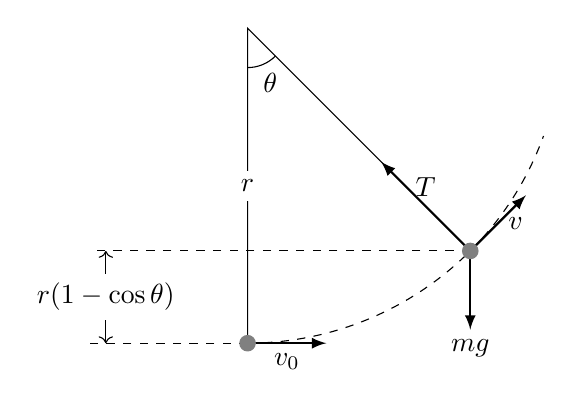
\begin{tikzpicture}
        \draw (0, -4) -- node[fill=white] {$r$} (0, 0) -- (-45:4);
        \draw[dashed] (-90:4) arc (-90:-20:4);
        \drawangle{(0, -4)}{(0, 0)}{(-45:4)};
        \draw[dashed] (0, -4) -- (-2, -4);
        \draw[dashed] (-45:4) -- (-2, {-2*sqrt(2)});
        \draw[<->] (-1.8, -4) -- node[fill=white] {$r(1-\cos\theta)$} (-1.8, {-2*sqrt(2)});
        \draw[thick, -latex] (0, -4) -- node[below] {$v_0$} ++ (1, 0);
        \fill[gray] (0, -4) circle (3pt);
        \draw[thick, -latex] (-45:4) -- node[right] {$v$} ++ ($0.5*(45:2)$);
        \draw[thick, -latex] (-45:4) -- node[above] {$T$} ++ ($0.8*(135:2)$);
        \draw[thick, -latex] (-45:4) -- ++ (0, -1) node[below] {$mg$};
        \fill[gray] (-45:4) circle (3pt);
    \end{tikzpicture}
    \caption{竖直平面圆周运动}
\end{figure}
将合力/加速度在平行和垂直运动方向上分解后可发现,垂直于运动方向的部分只负责维持各个瞬间的圆周运动,而平行于运动方向的部分只负责调整速度。此外,运动的物体只受重力(保存力)和绳子的拉力,而拉力时时刻刻又与运动方向垂直(不做功),所以整个系统机械能守恒。

\subparagraph{拉力大小}
\begin{align*}
    T=&G\cos\theta+m\frac{v^2}{r}\\
    \downarrow&\quad\frac12m{v_0}^2=\frac12mv^2+mgr(1-\cos\theta)\\
    =&mg\cos\theta+\frac{m{v_0}^2}{r}-2mg(1-\cos\theta)\\
    =&\frac{m{v_0}^2}{r}+mg(3\cos\theta-2)
\end{align*}

\subparagraph{最小初速度}
\begin{equation*}
    \begin{cases}
        \frac12m{v_0}^2=\frac12mv^2+2mgr\\
        mg=m\frac {v^2}r
    \end{cases}
    \implies v_{min}=v_0=\sqrt{5gr}
\end{equation*}

\paragraph{其他变形}在实际题目中除了用绳线做牵引,还有一些其他相似模型。
\begin{figure}[ht!]
    \centering
    \renewcommand\arraystretch{1.2}
    \begin{tabular}{c|cc}
        \hline
        牵引物&半周前&半周后\\\hline
        线/圆筒面&拉力&无\\
        棒/管内&拉力&支持力\\\hline
    \end{tabular}
    \caption{非等速圆周运动模型}
\end{figure}

\subsection{简谐振动}

\subsubsection{基本概念}

首先考虑如下模型:物体在平面上做等速圆周运动,其一侧有光源,另一侧有一光屏,观察光屏上点的运动模式。
\begin{figure}[ht!]
    \centering
    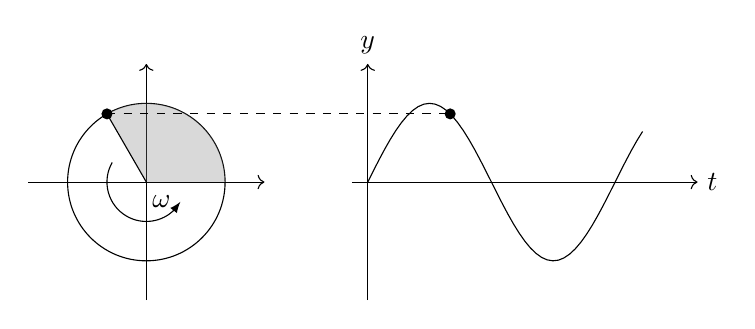
\begin{tikzpicture}
        \begin{scope}[xshift=-80]
            \draw[->] (-1.5, 0) -- (1.5, 0);
            \draw[->] (0, -1.5) -- (0, 1.5);
            \draw (0, 0) circle (1);
            \fill[fill=gray, opacity=0.3] (0, 0) -- (1, 0) arc (0 : 120 : 1) --cycle;
            \coordinate (P) at (120 : 1);
            \fill (P) circle (2pt);
            \draw (0, 0) -- (P);
            \draw[-latex] (150:0.5) arc (150:330:0.5) node[left] {$\omega$};
        \end{scope}
        \begin{scope}
            \draw[->] (-0.2, 0) -- ({rad(240)}, 0) node[right] {$t$};
            \draw[->] (0, -1.5) -- (0, 1.5) node[above] {$y$};
            \draw[domain=0:rad(200)] plot[samples=50] (\x, {sin(2*\x r)});
            \coordinate (Q) at ({rad(60)}, {sin(60)});
            \fill (Q) circle (2pt);
        \end{scope}
        \draw[dashed] (P) -- (Q);
    \end{tikzpicture}
    \caption{简谐振动}
\end{figure}
可见该点的位置(y坐标)与时间呈三角函数关系。这种物理量与时间呈三角函数关系的运动即为\underline{简谐振动},日文为単振動。其运动学信息可由等速圆周运动轻松求得。
\begin{itembox}[l]{简谐振动的运动学信息}
    \begin{itemize}
        \item 位移:$x=A\sin(\omega t+\theta_0)$
        \item 速度:$v=A\omega\cos(\omega t+\theta_0)$
        \item 加速度:$a=-A\omega^2\sin(\omega t+\theta_0)=-\omega^2x$
    \end{itemize}
\end{itembox}

\subsubsection{回复力}

结合牛二定律可见,做简谐振动的物体始终都会受到一个与位移方向相反的力,名为\underline{回复力},日文为復元力。因为位移的方向是以振动中心为基准向外的,所以回复力的方向即是始终指向其振动中心。
\begin{itembox}[l]{回复力}
    \begin{equation*}
        F=ma=-m\omega^2x=-kx\quad(k=m\omega^2)
    \end{equation*}
    \begin{itemize}
        \item $F\propto x$
        \item 方向指向振动中心
    \end{itemize}
\end{itembox}
此外,回复力的数学形式与弹簧弹力相像,所以不难推断回复力做功也与路径无关,属于保存力。因此简谐振动也满足机械能守恒。

虽然简谐振动中角速度不存在实际意义,但利用$T=\frac{2\pi}{\omega}$的关系,我们就可以得到简谐振动的周期。
\begin{itembox}[l]{简谐振动周期}
    \begin{equation*}
        T=2\pi\sqrt{\frac{m}{k}}
    \end{equation*}
\end{itembox}

\subsubsection{弹簧振子}

日文为バネ振り子,是最常见的简谐振动模型。
\begin{figure}[ht!]
    \centering
    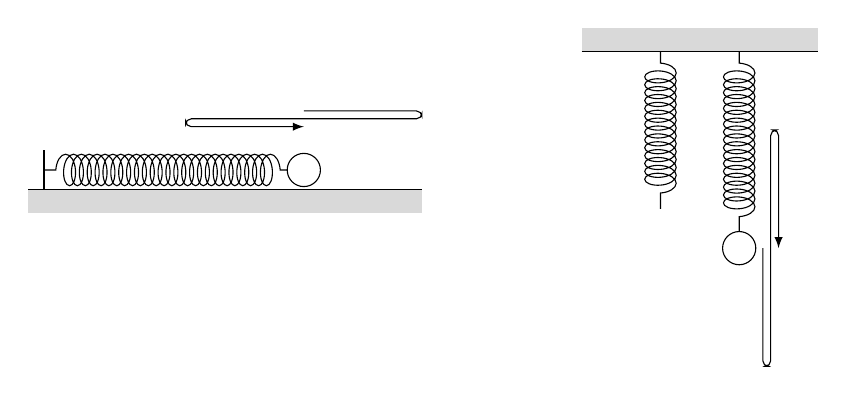
\begin{tikzpicture}
        \begin{scope}
            \draw (0, 0) -- (5, 0);
            \fill[fill=gray, opacity=0.3] (0, 0) rectangle (5, -0.3);
            \draw (0.2, 0) -- (0.2, 0.5);
            \draw[spring] (0.2, 0.25) -- ++ (3.2, 0);
            \draw[fill=white] (3.5, 0.25) circle (6pt);
            \draw[-latex, rounded corners=2pt] (3.5, 1) -- (5, 1) -- (5, 0.9) -- (2, 0.9) -- (2, 0.8) -- (3.5, 0.8);
        \end{scope}
        \begin{scope}[xshift=200, yshift=50]
            \draw (0, 0) -- (3, 0);
            \fill[fill=gray, opacity=0.3] (0, 0) rectangle (3, 0.3);
            \draw[spring] (1, 0) -- ++ (0, -2);
            \draw[spring] (2, 0) -- ++ (0, -2.3);
            \draw[fill=white] (2, -2.5) circle (6pt);
            \draw[-latex, rounded corners=2pt] (2.3, -2.5) -- (2.3, -4) -- (2.4, -4) -- (2.4, -1) -- (2.5, -1) -- (2.5, -2.5);
        \end{scope}
    \end{tikzpicture}
    \caption{弹簧振子}
\end{figure}
对于水平放置的弹簧,其回复力就是弹簧弹力,振动中心为原长处。对于竖直放置的情况受力分析后,可列如下等式。
\begin{align*}
    F=&mg-kx\\
    \downarrow&\quad mg=kx_0\\
    =&-k(x-x_0)
\end{align*}
即回复力中的k值仍旧是弹簧的弹性系数,振动中心下移至了平衡位置。更一般的,对于任意形式放置的弹簧上述结论皆成立。

\subsubsection{单摆}

日文为単振り子,属于摆动幅度极小的竖直平面圆周运动的模型。
\begin{figure}[ht!]
    \centering
    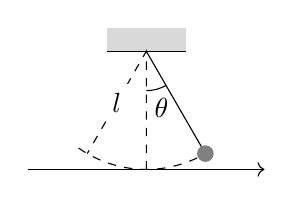
\begin{tikzpicture}
        \draw (-0.5, 0) -- (0.5, 0);
        \fill[fill=gray, opacity=0.3] (-0.5, 0) rectangle (0.5, 0.3);
        \draw[->] (-1.5, -1.5) -- (1.5, -1.5);
        \draw[dashed] (-125:1.5) arc (-125:-55:1.5);
        \draw (-60:1.5) -- (0, 0);
        \draw[dashed] (-90:1.5) -- (0, 0) -- node[fill=white] {$l$} (-120:1.5);
        \drawangle{(-90:1.5)}{(0, 0)}{(-60:1.5)};
        \fill[fill=gray] (-60:1.5) circle (3pt);
    \end{tikzpicture}
    \caption{单摆}
\end{figure}
鉴于其周期推导略复杂,这里直接给出结论。
\begin{itembox}[l]{单摆周期公式}
    \begin{equation*}
        T=2\pi\sqrt{\frac{l}{g}}
    \end{equation*}
\end{itembox}

\subsection{天体运动}

\subsubsection{开普勒定律}

开普勒定律是开普勒基于其老师第谷的实验数据总结而得的。而且此定律不仅适用于恒星与其行星之间,行星与其卫星也同样适用。
\begin{itembox}[l]{开普勒定律}
    \begin{itemize}
        \item 轨道法则:行星运动在以恒星为焦点的椭圆轨道上
        \item 面积法则:行星与恒星连线的$\begin{cases}\textrm{在单位时间内扫过的面积}\\\textrm{面积速度}\end{cases}$相等
        \item 周期法则:$T^2=ka^3\quad(k:const)$
    \end{itemize}
\end{itembox}
\begin{figure}[ht!]
    \centering
    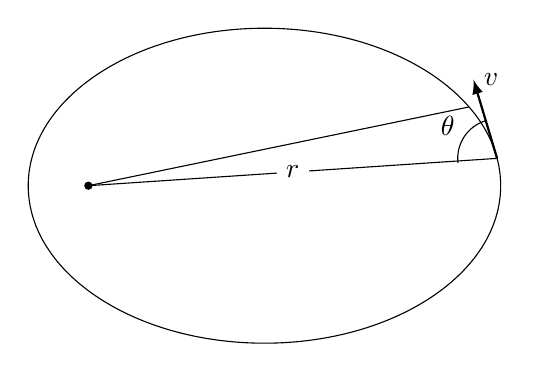
\begin{tikzpicture}
        \fill ({-sqrt(5)}, 0) circle (1.5pt);
        \draw (0, 0) circle (3 and 2);
        \draw ({-sqrt(5)}, 0) -- node[fill=white] {$r$} ++ ($({sqrt(5)}, 0)+(10:3 and 2)$);
        \draw ({-sqrt(5)}, 0) -- ++ ($({sqrt(5)}, 0)+(30:3 and 2)$);
        \draw[thick, -latex] (10:3 and 2) -- ++ (-0.3, 1) node[right] {$v$};
        \drawangle{($(10:3 and 2)+(-0.3, 1)$)}{(10:3 and 2)}{(0, 0)};
    \end{tikzpicture}
    \caption{面积速度}
\end{figure}
\begin{itembox}[l]{面积速度}
    \begin{equation*}
        \frac{dS}{dt}=\frac{\frac12r(v\cdot dt\sin\theta)}{dt}=\frac12rv\sin\theta
    \end{equation*}
\end{itembox}

\subsubsection{万有引力定律}

\paragraph{万有引力}是牛顿根据开普勒第三定律的思想发展出来的,描述物体间引力的理论。
\begin{itembox}[l]{万有引力公式}
    \begin{equation*}
        F=G\frac{m_1m_2}{r^2}\quad(\textrm{万有引力定数:}G=6.67\times10^{-11}N\cdot m^2\cdot kg^{-2})
    \end{equation*}
\end{itembox}
在实际运算过程中,一般将地表附近的万有引力视为重力。
\begin{itembox}[l]{黄金代换式}
    \begin{equation*}
        G\frac{Mm}{R^2}=mg\implies
        GM=gR^2
    \end{equation*}
\end{itembox}
但严格意义上讲,由于地球自转,地表上的物体还会受到离心力(非惯性系)。因此,实际的g值会比黄金代换式求得的值小一些。
\begin{figure}[ht!]
    \centering
    \begin{tikzpicture}[scale=0.8]
        \fill (0, 0) circle (1.5pt);
        \draw (0, 0) circle (2);
        \draw[thick, -latex] (45:2) -- (45:1) node[left] {万有引力};
        \draw[thick, -latex] (45:2) -- ($(45:2)+(0.5,0)$) node[right] {离心力};
        \draw[thick, -latex] (45:2) -- ($(45:1)+(0.5,0)$) node[below] {重力};
    \end{tikzpicture}
    \caption{万有引力与重力}
\end{figure}

\paragraph{万有引力势能}与重力类似,万有引力也有其对应的势能,为方便运算一般取无限远处为势能基准点。
\begin{figure}[ht!]
    \centering
    \begin{tikzpicture}[scale=0.8]
        \filldraw[color=black, fill=gray, fill opacity=0.3] (-30:1.5) arc (-30:210:1.5);
        \draw (-4, 0) -- (2, 0);
        \draw[->] (0, 0) -- (0, 4) node[right] {正};
        \draw[dashed] (0, 4) -- (-3, 4);
        \draw[<->] (-3, 0) -- node[fill=white] {$\infty$} (-3, 4);
        \draw[dashed] (0, 3) -- (-2, 3);
        \draw[<->] (-2, 0) -- node[fill=white] {$r$} (-2, 3);
        \draw[thick, -latex] (0, 3) -- node[right] {万有引力} (0, 2);
        \fill[fill=gray, opacity=0.5] (0, 3) circle (5pt);
    \end{tikzpicture}
    \caption{万有引力势能}
\end{figure}
\begin{itembox}[l]{万有引力势能(万有引力による位置エネルギー)}
    \begin{equation*}
        E_p=-G\frac{Mm}{r}
    \end{equation*}
\end{itembox}

\paragraph{应用}基于万有引力和万有引力势能即可试求两个宇宙速度。
\begin{figure}[ht!]
    \centering
    \begin{tikzpicture}
        \fill[fill=gray, opacity=0.3] (0, 0) circle (1.2);
        \draw[thick, -latex] (90:1.4) arc (90:-260:1.4) node[left, above] {第一宇宙速度};
        \draw[thick, -latex] (90:1.4) arc (90:0:2 and 3) node[right] {第二宇宙速度};
    \end{tikzpicture}
    \caption{宇宙速度}
\end{figure}

\subparagraph{第一宇宙速度}能够围绕地球旋转的最小速度。
\begin{equation*}
    m\frac{v^2}{r}=G\frac{Mm}{r^2}\implies
    v=\sqrt{gr}
\end{equation*}

\subparagraph{第二宇宙速度}能够挣脱地球引力的最小速度。
\begin{equation*}
    \frac12mv^2-G\frac{Mm}{r}=0(E_k)+0(E_p)\implies
    v=\sqrt{2gr}
\end{equation*}


    % chapter 2

\chapter{热学}

% chapter 2 section 1

\section{热与能量}

\paragraph{热}即是宏观上物体处于静止状态,但其中构成该物体的分子仍然在做着随机、杂乱无章的运动,即\underline{热运动}。在这个过程中分子彼此不断碰撞,交换着热运动时所具有的能量。这些转移在分子间的热运动的能量就是所谓的\underline{热}或是\underline{热能},日文为熱/熱エネルギー。

\paragraph{温度}由于一般的观察只能停留于宏观层面,很难真正地去计算分子间实际交换的能量,所以我们用温度这个宏观物理量去描述粒子的微观信息。
\begin{itembox}[l]{开氏温度}
    \centering
    絶対温度$T=t+273(K)$
\end{itembox}
\begin{itembox}[l]{热容量与比热}
    \begin{itemize}
        \item 热容量:物体升高1K所需的热量
        \item 比热:单位质量的物体升高1K所需的热量,物体单位质量的热容量
    \end{itemize}
    \begin{gather*}
        C=m\cdot c\\
        \Delta Q=C\cdot\Delta t=c\cdot m\cdot\Delta t
    \end{gather*}
\end{itembox}

\paragraph{断热容器}是不与周边物体做热交换的容器。在这样的环境下,容器内的物体只会与彼此传递热量,从而达到了整体热量不增不减的效果,即\underline{热量守恒},日文为熱量保存。
\begin{itembox}[l]{热量守恒定律}
    \begin{itemize}
        \item 系统中吸热=系统中放热
        \item $Q_\textrm{吸}=Q_\textrm{放}$
    \end{itemize}
\end{itembox}

\paragraph{潜热}在物体发生三态变化时,会有一段持续吸热/放热但温度不变的过程。因为物体的温度仅取决于内部分子的动能,然而物体改变状态时只有其分子间力引起的势能发生变化,所以虽然吸热/放热但温度不增减。我们将这个期间内吸收/放出的热量称为\underline{潜热}。常有融解热、蒸发热。
\begin{figure}[ht!]
    \centering
    \begin{tikzpicture}
        \node[draw, circle] (A) at (0, 0) {固态};
        \node[draw, circle] (B) at (60:3.6) {气态};
        \node[draw, circle] (C) at (3.6, 0) {液态};
        \draw[thick, <->] (A) -- node[fill=white] {昇華 昇華} (B);
        \draw[thick, <->] (A) -- node[fill=white] {凝固 融解} (C);
        \draw[thick, <->] (B) -- node[fill=white] {凝縮 蒸発} (C);
    \end{tikzpicture}
    \caption{三态变化}
\end{figure}

% chapter 2 section 2

\section{气体分子运动}

\paragraph{气体压强}日文为気体の圧力,由于气体分子冲撞(假想的)接触面而成,单位为帕斯卡(Pa)。
\begin{equation*}
    P=\frac{F}{S}
\end{equation*}

\subsection{气体法则}
\label{subsec:2.2.1}

\begin{itembox}[l]{波意尔查理定律}
    \begin{itemize}
        \item 波意尔定律(ボイルの法則)
        \begin{equation*}
            T=const\implies P\cdot V=const
        \end{equation*}
        \item 查理定律(シャルルの法則)
        \begin{equation*}
            P=const\implies\frac{V}{T}=const
        \end{equation*}
        \item 波意尔查理定律(ボイル・シャルルの法則)
        \begin{equation*}
            \frac{PV}{T}=const
        \end{equation*}
    \end{itemize}
\end{itembox}
\begin{figure}[ht!]
    \centering
    \begin{minipage}[t]{0.48\textwidth}
        \centering
        \begin{tikzpicture}[scale=0.8]
            \draw[->] (0, 0) -- (0, 3) node[above] {$P$};
            \draw[->] (0, 0) -- (3, 0) node[right] {$V$};
            \draw[thick, domain=0.18:2.7] plot (\x, {0.5/\x}) node[above] {低温};
            \draw[thick, domain=0.74:2.7] plot (\x, {2/\x}) node[above] {高温};
        \end{tikzpicture}
        \caption{波意尔定律}
    \end{minipage}
    \begin{minipage}[t]{0.48\textwidth}
        \centering
        \begin{tikzpicture}[scale=0.8]
            \draw[->] (0, 0) -- (0, 3) node[above] {$V$};
            \draw[->] (0, 0) -- (3, 0) node[right] {$T$};
            \draw[thick, dashed] (0, 0) -- (0.5, 0.5);
            \draw[thick] (0.5, 0.5) -- (2.7, 2.7);
        \end{tikzpicture}
        \caption{查理定律}
    \end{minipage}
\end{figure}

\paragraph{理想气体状态方程}\underline{理想气体}即忽略分子间力,严格满足波意尔查理定律的气体。因此,当一般气体处于\underline{高温+低压}的环境下时会表现得像理想气体。拓展波意尔查理定律后可得普适于理想气体的方程。
\begin{itembox}[l]{理想气体状态方程}
    \begin{equation*}
        PV=nRT\quad(R\textrm{:気体定数})
    \end{equation*}
\end{itembox}

\subsection{热力学第一定律}
\label{subsec:2.2.2}

\subsubsection{气体内能}

分子热运动的动能和由分子间力产生的势能共同构成一般的气体内能。由于理想气体忽略了其分子间力,所以理想气体的内能就等于其分子动能之和。
\begin{itembox}[l]{气体内能}
    \begin{equation*}
        U=\frac32nRT=\frac32PV\quad(U\propto T)
    \end{equation*}
\end{itembox}

\subsubsection{热力学第一定律}

一般有两种方式可以改变物体的内能:
\begin{itemize}
    \item 吸热/放热
    \item 做功/被做功
\end{itemize}
操作热的方式十分直观:通过宏观温度直接改变内能。另一方面,让气体做功的方式是通过其体积的改变来实现内能变化的。
\begin{itembox}[l]{气体做功}
    \begin{equation*}
        W=F\cdot\Delta x=PS\cdot\Delta x=P\Delta V
    \end{equation*}
    \begin{itemize}
        \item 压缩:$\Delta U>0$
        \item 膨胀:$\Delta U<0$
    \end{itemize}
\end{itembox}
于是将这两种改变内能的方式结合在一起便有了热力学第一定律的内容。
\begin{figure}[ht!]
    \centering
    \begin{minipage}[t]{0.48\textwidth}
        \centering
        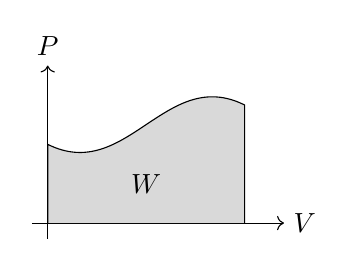
\begin{tikzpicture}
            \draw[->] (-0.2, 0) -- (3, 0) node[right] {$V$};
            \draw[->] (0, -0.2) -- (0, 2) node[above] {$P$};
            \filldraw[color=black, fill=gray, fill opacity=0.3] (0, 0) -- 
                (0, 1) .. controls (1, 0.5) and (1.5, 2) .. (2.5, 1.5) -- (2.5, 0);
            \node at (1.25, 0.5) {$W$};
        \end{tikzpicture}
        \caption{气体做功}
    \end{minipage}
    \begin{minipage}[t]{0.48\textwidth}
        \centering
        \begin{tikzpicture}
            \draw[thick] (0, 2) -- (0.3, 2) {[rounded corners=5pt] -- (0.3, 0.3) -- (1.5, 0.3)} -- (1.5, 2) -- (1.8, 2) {[rounded corners=5pt] -- (1.8, 0) -- (0, 0)} -- cycle {};
            \filldraw[color=black, fill=gray, fill opacity=0.3] (0.3, 1.7) -- (1.5, 1.7) -- (1.5, 1.5) -- (0.3, 1.5) -- cycle;
            \draw[ultra thick, -latex] (0.9, -0.2) -- (0.9, 0.8);
            \draw[ultra thick, -latex] (0.9, 2) -- (0.9, 1);
            \node at (0.9, -0.5) {热量Q};
            \node at (0.9, 2.3) {功W};
        \end{tikzpicture}
        \caption{热力学第一定律}
    \end{minipage}
\end{figure}
\begin{itembox}[l]{热力学第一定律}
    \begin{equation*}
        \Delta U=Q_\textrm{吸}+W_\textrm{された}
    \end{equation*}
\end{itembox}

\subsection{气体状态变化}
\label{subsec:2.2.3}

分别固定气体的体积、压强、温度等物理量,我们能够得到以下几种典型状态变化。

\paragraph{等积变化}保持气体体积不变的变化。
\begin{itemize}
    \item $W=P\Delta V=0$
    \item $Q_\textrm{吸}=\Delta U=\frac32nR\Delta T=nC_v\Delta T$
    \item $C_v=\frac32R$:定積モル比熱
\end{itemize}

\paragraph{等压变化}保持气体压强不变的变化。
\begin{itemize}
    \item $W=P\Delta V=nR\Delta T$
    \item $Q_\textrm{吸}=\Delta U+W_\textrm{した}=\frac52nR\Delta T=nC_p\Delta T$
    \item $C_p=\frac52R$:定圧モル比熱
\end{itemize}

\paragraph{等温变化}保持气体温度不变的变化。
\begin{itemize}
    \item $\Delta U=0$
    \item $Q_\textrm{吸}=W_\textrm{した}$
\end{itemize}

\paragraph{断热变化}保持气体吸热为0的变化。
\begin{itemize}
    \item $Q_\textrm{吸}=0$
    \item $\Delta U=W_\textrm{された}$
    \begin{itemize}
        \item 断热膨胀:T减少,U减少
        \item 断热压缩:T增大,U增大
    \end{itemize}
\end{itemize}

\begin{figure}[ht!]
    \centering
    \begin{minipage}[t]{0.48\textwidth}
        \centering
        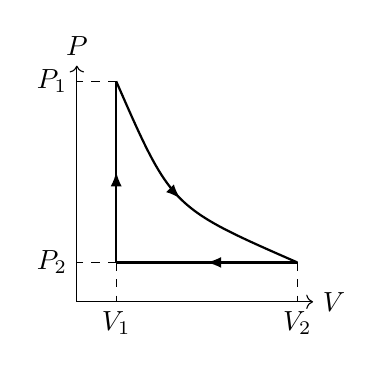
\begin{tikzpicture}
            \draw[->] (0, 0) -- (0, 3) node[above] {$P$};
            \draw[->] (0, 0) -- (3, 0) node[right] {$V$};
            \coordinate (p1v1) at (0.5, 2.8);
            \coordinate (p2v1) at (0.5, 0.5);
            \coordinate (p2v2) at (2.8, 0.5);
            \draw[thick, midarrow] (p2v1) -- (p1v1);
            \draw[thick, midarrow] (p2v2) -- (p2v1);
            \draw[thick, midarrow] (p1v1) .. controls (1.2, 1.2) .. (p2v2);
            \draw[dashed] (p1v1) -- (0, 2.8) node[left] {$P_1$};
            \draw[dashed] (p2v1) -- (0, 0.5) node[left] {$P_2$};
            \draw[dashed] (p2v1) -- (0.5, 0) node[below] {$V_1$};
            \draw[dashed] (p2v2) -- (2.8, 0) node[below] {$V_2$};
        \end{tikzpicture}
        \caption{气体状态变化}
    \end{minipage}
    \begin{minipage}[t]{0.48\textwidth}
        \centering
        \begin{tikzpicture}
            \draw[->] (0, 0) -- (0, 3) node[above] {$P$};
            \draw[->] (0, 0) -- (3, 0) node[right] {$V$};
            \draw[dashed, domain=0.37:2.7] plot (\x, {1/\x});
            \draw[dashed, domain=0.74:2.7] plot (\x, {2/\x});
            \draw[thick, midarrow] (0.74, 2.7) .. controls (1.2, 1.2) .. (2.5, 0.4);
        \end{tikzpicture}
        \caption{断热变化}
    \end{minipage}
\end{figure}

\subparagraph{断热自由膨胀}

一断热容器由挡板分隔为左右两部分,其中左侧空腔注有理想气体,右侧为真空。打开隔板,左侧气体自由扩散至右侧,最终充满整个容器。整个过程中气体扩散无有阻碍,因此不存在做功,加之容器断热,根据热力学第一定律可知整个系统能量不变。
\begin{itemize}
    \item $Q=W=0\implies\Delta U=0\implies\Delta T=0$
    \item $P_1V_1=P_2V_2$
\end{itemize}
\begin{figure}[ht!]
    \centering
    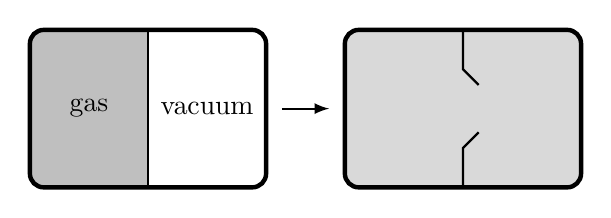
\begin{tikzpicture}
        \begin{scope}
            \fill [fill=gray, opacity=0.5] (1.5, 0) -- ++ (0, 2) {[rounded corners=5pt] -- ++(-1.5, 0) -- ++ (0, -2)} -- cycle {};
            \draw[ultra thick, rounded corners=5pt] (0, 0) rectangle (3, 2);
            \draw[thick] (1.5, 0) -- (1.5, 2);
            \node at (0.75, 1) {gas};
            \node at (2.25, 1) {vacuum};
            \draw[thick, -latex] (3.2, 1) -- (3.8, 1);
            \filldraw[ultra thick, rounded corners=5pt, color=black, fill=gray, fill opacity=0.3] (4, 0) rectangle (7, 2);
            \draw[thick] (5.5, 0) -- (5.5, 0.5) -- ++ (0.2, 0.2);
            \draw[thick] (5.5, 2) -- (5.5, 1.5) -- ++ (0.2, -0.2);
        \end{scope}
    \end{tikzpicture}
    \caption{断热自由膨胀}
\end{figure}

\subparagraph{断热气体混合}

与断热自由膨胀类似,只不过将断热容器的右侧空腔也注入理想气体,打开活塞后两种气体混合。从整体出发,硬质容器不发生体积变化且断热,因此根据热力学第一定律可得内部气体总内能不发生改变。
\begin{gather*}
    U_A+U_B=U\\
    \frac32n_ART_A+\frac32n_BRT_B=\frac32(n_A+n_B)RT\\
    T=\frac{n_AT_A+n_BT_B}{n_A+n_B}
\end{gather*}
\begin{figure}[ht!]
    \centering
    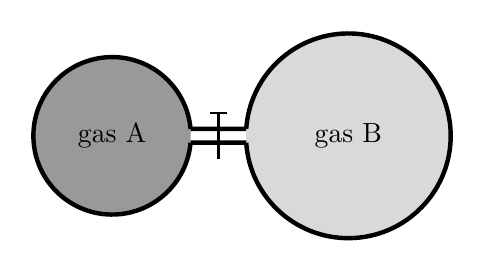
\begin{tikzpicture}
        \filldraw[ultra thick, color=black, fill=gray, fill opacity=0.8] (5:1) arc (5:355:1);
        \filldraw[ultra thick, color=black, fill=gray, fill opacity=0.3] ($(3, 0)+(-176.15:1.3)$) arc (-176.15:176.15:1.3);
        \draw[ultra thick] (5:1) -- ($(3, 0)+(176.15:1.3)$);
        \draw[ultra thick] (-5:1) -- ($(3, 0)+(-176.15:1.3)$);
        \draw[thick, |-] (1.35, 0.3) -- (1.35, -0.3);
        \node at (0, 0) {gas A};
        \node at (3, 0) {gas B};
    \end{tikzpicture}
    \caption{断热气体混合}
\end{figure}

\paragraph{热效率}吸热做功的机械为热机,其热到功的转化率为热效率。
\begin{itembox}[l]{热效率}
    \begin{equation*}
        \eta=\frac{W_\textrm{实际}}{Q_\textrm{吸}}
        =\frac{W_\textrm{した}-W_\textrm{された}}{Q_\textrm{吸}}
    \end{equation*}
\end{itembox}


    % chapter 3

\chapter{波动}

% chapter 3 section 1

\section{波的性质}

\subsection{波的传播}

\subsubsection{波}

波即某种物理信息在空间中传播的现象。例如我们拿住一根绳子的一端,把其另一端固定在墙面上,抖动握持的一端,这便形成了一种简单的波。
\begin{figure}[ht!]
    \centering
    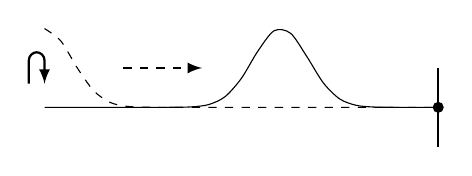
\begin{tikzpicture}
        \draw[thick] (5, 0.5) -- (5, -0.5);
        \fill (5, 0) circle (2pt);
        \draw[rounded corners=3pt, thick, -latex] (-0.2, 0.3) -- (-0.2, 0.7) -- (0, 0.7) -- (0, 0.3);
        \draw[dashed, domain=0:5] plot[smooth] (\x, {exp(-4*\x^2)});
        \draw[domain=0:5] plot[smooth] (\x, {exp(-4*(\x-3)^2)});
        \draw[thick, dashed, -latex] (1, 0.5) -- (2, 0.5);
    \end{tikzpicture}
    \caption{波的形成}
\end{figure}
将其中传递波的事物称为\underline{介质},日文为媒質。在上述例子中介质就是绳子上的每一段绳结。以下是一些描述波的时候常用的物理量。
\begin{itemize}
    \item 波形:描述某时刻波上各点状态的曲线
    \item 波速$v$:日文为波の速さ,即波的传播速度
    \item 波峰/波谷:日文为山/谷,即波形上的最高处/最低处
    \item 波长$\lambda$:相邻的波峰间的距离
    \item 振幅$A$:介质振动的位移
    \item 周期$T$:等同于介质的振动周期
    \item 频率$f$:日文为振動数,周期的倒数
\end{itemize}
基于上述信息便可得到波的基本公式。
\begin{itembox}[l]{波的基本公式}
    \begin{equation*}
        v=\frac{\lambda}{T}=\lambda f
    \end{equation*}
\end{itembox}

\subsubsection{横波与纵波}

\paragraph{定义}根据介质的振动方向和波的传播方向的关系,可以如下对波进行分类。
\begin{itemize}
    \item 横波:振动方向与传播方向垂直的波
    \item 纵波:振动方向与传播方向平行的波
\end{itemize}
其中纵波会呈现明显的疏密变化,所以也叫做疏密波。

\paragraph{描绘}对于横波,我们可以通过将各个介质的位置描绘在坐标平面上的方式来十分轻松地记录其波形等信息。然而若是使用相同的方式(逐个描点)去记录纵波则会发现所有点都聚集在x轴上,很难对其进行清晰地梳理。为此,我们仍然使用横波的绘图方式,只是对每个点的含义做重新诠释,使其能够更好地展现纵波的特征。
\begin{figure}[ht!]
    \centering
    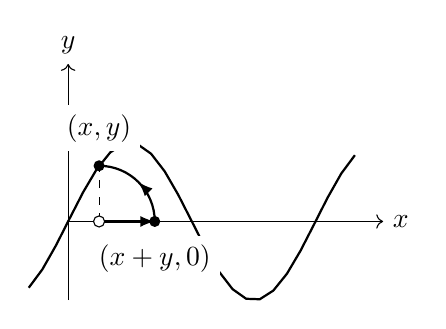
\begin{tikzpicture}
        \draw[->] (0, -1) -- (0, 2) node[above] {$y$};
        \draw[->] (0, 0) -- (4, 0) node[right] {$x$};
        \draw[thick, domain=-0.5:{pi+0.5}] plot (\x, {sin(2*(\x r))});
        \draw[dashed] ({pi/8}, 0) -- ({pi/8}, {sin(pi/4 r)});
        \draw[thick, -latex] ({pi/8}, 0) -- ({pi/8+sin(pi/4 r)}, 0);
        \draw[thick, midarrow] ({pi/8+sin(pi/4 r)}, 0) arc (0:90:{sin(pi/4 r)});
        \filldraw[color=black, fill=white] ({pi/8}, 0) circle (2pt);
        \fill ({pi/8+sin(pi/4 r)}, 0) circle (2pt);
        \fill ({pi/8}, {sin(pi/4 r)}) circle (2pt);
        \node[below=5pt, fill=white] at ({pi/8+sin(pi/4 r)}, 0) {$(x+y,0)$};
        \node[above=5pt, fill=white] at ({pi/8}, {sin(pi/4 r)}) {$(x,y)$};
    \end{tikzpicture}
    \caption{纵波的图示}
\end{figure}
对于纵波上原本在$(x,0)$点的介质,倘若在某一时刻它关于自身的基准位置发生了$y$大小的偏移,那么根据纵波的定义,该点当前的坐标将会是$(x+y,0)$。既然如此,我们则可以将该点的基准位置信息和振动信息分离,让x轴和y轴分别来呈现,也就是将这个介质描绘在$(x,y)$处。得益于这种表现方式,我们就可以更容易地判断纵波的疏部与密部的位置了。比如\tikz{\draw (-0.2,-0.2) cos (0,0) -- (0,0) sin (0.2,0.2);}的部分,其中左侧部分介质负向偏移、右侧部分正向偏移,中点两侧的介质均往两侧远离,因此这里是疏部。另一种情况也是如此的分析方式。

\subsubsection{波的解析式}

至此不难发现波上每一个介质的振动情况是依存于当前的时间和其在空间上的位置的,因此为了准确描述任意时刻波上任意位置的介质的位置就需要用形如$y=f(x,t)$的函数才能完成。
\begin{figure}[ht!]
    \centering
    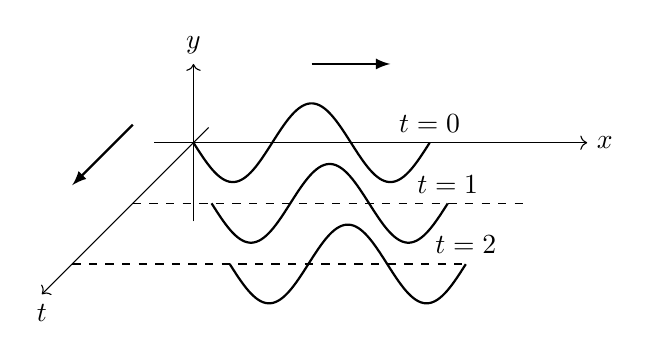
\begin{tikzpicture}
        \draw[->] (0,0,-0.5) -- (0,0,5) node[below] {$t$};
        \draw[->] (-0.5,0,0) -- (5,0,0) node[right] {$x$};
        \draw[->] (0,-1,0) -- (0,1,0) node[above] {$y$};
        \draw[thick, -latex] (1.5,1,0) -- (2.5,1,0);
        \draw[thick, -latex] (0,1,2) -- (0,1,4);
        \draw[thick] plot[variable=\x,domain=0:3, samples=100,smooth] (\x, {sin((pi*(0-\x)) r)/2}, 0) node[above] {$t=0$};
        \draw[dashed] (0,0,2) -- (5,0,2);
        \draw[thick] plot[variable=\x,domain=1:4, samples=100,smooth] (\x, {sin((pi*(1-\x)) r)/2}, 2) node[above] {$t=1$};
        \draw[dashed] (0,0,4) -- (5,0,4);
        \draw[thick] plot[variable=\x,domain=2:5, samples=100,smooth] (\x, {sin((pi*(2-\x)) r)/2}, 4) node[above] {$t=2$};
    \end{tikzpicture}
    \caption{波的解析式}
\end{figure}
于是,基于波的定义,我们可以从波源着手来推导正弦波的解析式。正弦波的波源做着简谐振动,假设其振动为$y=A\sin(\omega t)$。那么,波源的振动将会在$\frac{x}{v}$时间后传播到波上处于$x$位置上的任意一点,因此该点的$y-t$振动图像就是波源振动图像向右平移$\frac{x}{v}$个单位后的样子。
\begin{itembox}[l]{波的解析式}
    \begin{align*}
        y(x)=&A\sin\left(\omega\left(t-\frac{x}{v}\right)\right)\\
        =&A\sin\left(2\pi\left(\frac{t}{T}-\frac{x}{\lambda}\right)\right)
    \end{align*}
\end{itembox}
其中$\sin$内部的内容叫做位相、波的传播方向可由$v$做调整。同样的,通过平移某一时刻$y-x$图像的方式也可以完成上述推导。

\subsection{波的干涉}

\paragraph{脉冲波}日文为パルス波パルス波,指的是由一组振动形成的波。
\begin{figure}[ht!]
    \centering
    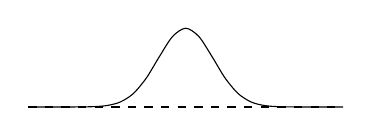
\begin{tikzpicture}
        \draw[dashed] (0,0) -- (4,0);
        \draw[domain=0:4] plot[smooth] (\x, {exp(-4*(\x-2)^2)});
    \end{tikzpicture}
    \caption{脉冲波}
\end{figure}

\subsubsection{波的叠加原理}

波在传播的过程中遵循\underline{叠加原理}和\underline{独立性原理}。即在与其他波相遇时会发生叠加,且满足$y=y_1+y_2$,在彼此分开后仍然保持叠加前的振动方式。
\begin{figure}[ht!]
    \centering
    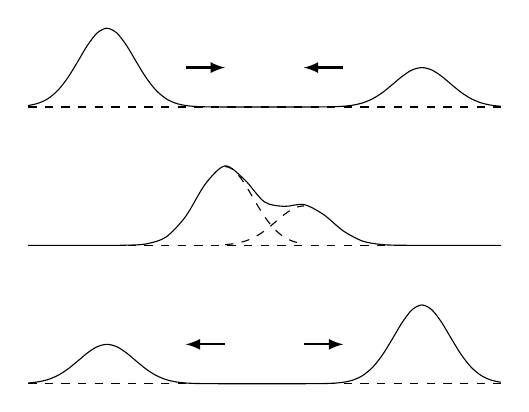
\begin{tikzpicture}
        \begin{scope}
            \draw[dashed] (0,0) -- (6,0);
            \draw[domain=0:3] plot[smooth] (\x, {exp(-4*(\x-1)^2)});
            \draw[domain=3:6] plot[smooth] (\x, {0.5*exp(-4*(\x-5)^2)});
            \draw[thick, -latex] (2,0.5) -- (2.5, 0.5);
            \draw[thick, -latex] (4,0.5) -- (3.5, 0.5);
        \end{scope}
        \begin{scope}[yshift=-50]
            \draw[dashed] (0,0) -- (6,0);
            \draw[dashed, domain=2.5:3.5] plot[smooth] (\x, {exp(-4*(\x-2.5)^2)});
            \draw[dashed, domain=2.5:3.5] plot[smooth] (\x, {0.5*exp(-4*(\x-3.5)^2)});
            \draw[domain=0:6] plot[smooth] (\x, {exp(-4*(\x-2.5)^2)+0.5*exp(-4*(\x-3.5)^2)});
        \end{scope}
        \begin{scope}[yshift=-100]
            \draw[dashed] (0,0) -- (6,0);
            \draw[domain=3:6] plot[smooth] (\x, {exp(-4*(\x-5)^2)});
            \draw[domain=0:3] plot[smooth] (\x, {0.5*exp(-4*(\x-1)^2)});
            \draw[thick, -latex] (2.5,0.5) -- (2, 0.5);
            \draw[thick, -latex] (3.5,0.5) -- (4, 0.5);
        \end{scope}
    \end{tikzpicture}
    \caption{波的叠加原理}
\end{figure}

\subsubsection{平面波的干涉}

设想平面上有两个同样的波源同时产生相同的波(周期、最大振幅、位相均相同)。倘若俯视观察平面,则会发现以波源为圆心形如同心圆样式的波纹。其中虚线代表波谷的波面,实线代表波峰的波面,即两个虚线之间的长度为一个波长。根据波的叠加原理分析可知这些波面会发生相互加强/减弱的现象,我们将其称为\underline{波的干涉}。
\begin{figure}[ht!]
    \centering
    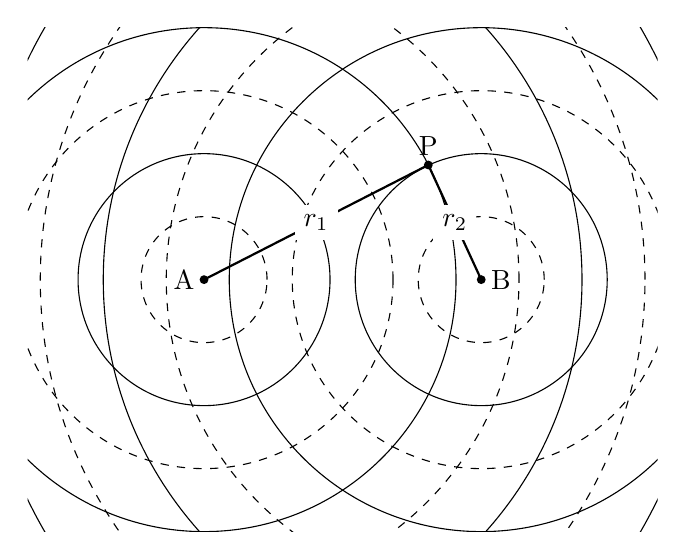
\begin{tikzpicture}[scale=0.8]
        \coordinate (A) at (-2.2,0);
        \coordinate (B) at (2.2,0);
        \coordinate (P) at (1.36,1.82);
        \clip (-5,-4) rectangle (5,4);
        \fill (A) circle (2pt) node[left] {A};
        \fill (B) circle (2pt) node[right] {B};
        \foreach \r in {1, 3, 5, 7} {
            \draw[dashed] (A) circle (\r);
            \draw[dashed] (B) circle (\r);
        }
        \foreach \r in {2, 4, 6, 8} {
            \draw (A) circle (\r);
            \draw (B) circle (\r);
        }
        \fill (P) circle (2pt) node[above] {P};
        \draw[thick] (A) -- node[fill=white] {$r_1$} (P);
        \draw[thick] (B) -- node[fill=white] {$r_2$} (P);
    \end{tikzpicture}
    \caption{平面波的干涉}
\end{figure}
总结平面上加强点、减弱点的规律可得波的干涉条件。
\begin{itembox}[l]{波的干涉条件}
    \begin{itemize}
        \item 加强:$|r_1-r_2|=2n\cdot\frac{\lambda}{2}$
        \item 减弱:$|r_1-r_2|=(2n+1)\cdot\frac{\lambda}{2}$
    \end{itemize}
\end{itembox}
其中的加强点,日文为腹,是两个波峰或者两个波谷叠加而得,均为整个波中振幅最大、振动最剧烈的位置,因此叠加后的结果也将会是振动最剧烈的位置。相反,减弱点,日文为節,是由波峰和波谷叠加而得,振幅相互抵消,因此叠加后将不会产生明显的振动。此外,观察干涉条件的数学形式:干涉点到两波源的差值一定,根据圆锥曲线的定义可知加强点/减弱点的连线为双曲线。

\subsubsection{驻波}

\begin{figure}[ht!]
    \centering
    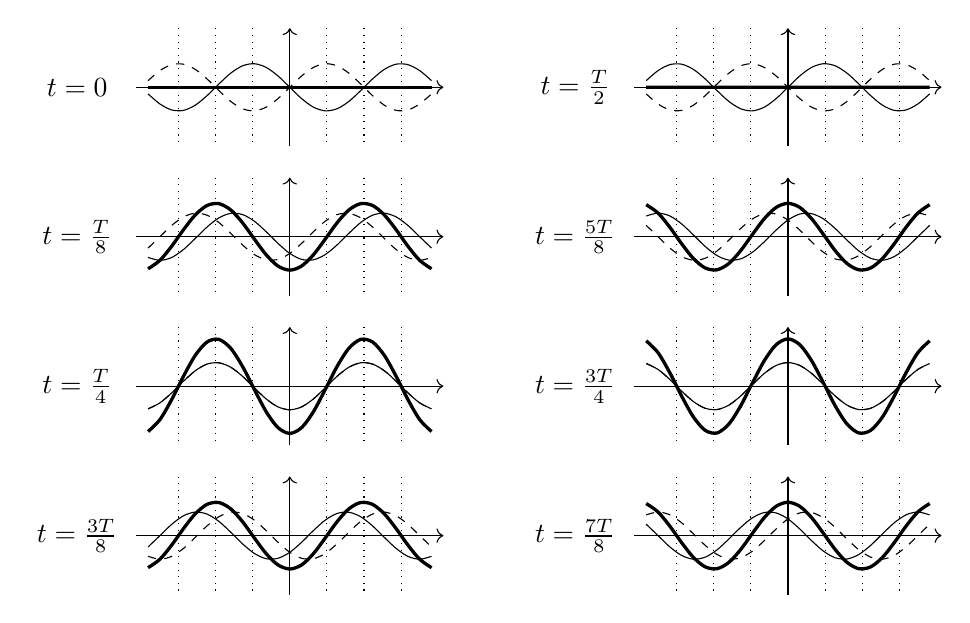
\begin{tikzpicture}
        \foreach \t/\shift/\xshift/\yshift in {
            $t=0$           /0       /0  /0,
            $t=\frac{T}{8}$ /{1*pi/4}/0  /-180,
            $t=\frac{T}{4}$ /{2*pi/4}/0  /-360,
            $t=\frac{3T}{8}$/{3*pi/4}/0  /-540,
            $t=\frac{T}{2}$ /{4*pi/4}/600/0,
            $t=\frac{5T}{8}$/{5*pi/4}/600/-180,
            $t=\frac{3T}{4}$/{6*pi/4}/600/-360,
            $t=\frac{7T}{8}$/{7*pi/4}/600/-540
        } {
            \begin{scope}[scale=0.3, xshift=\xshift, yshift=\yshift]
                \draw[->] (0,-2.5) -- (0,2.5);
                \draw[->] (-6.5,0) -- (6.5,0);
                \node at (-9,0) {\t};
                \draw[dashed, domain=-6:6] plot[smooth] (\x, {sin((\x-\shift) r)});
                \draw[solid, domain=-6:6] plot[smooth] (\x, {-sin((\x+\shift) r)});
                \draw[very thick, domain=-6:6] plot[smooth] (\x, {sin((\x-\shift) r)-sin((\x+\shift) r)});
                \foreach \x in {
                    {-1*pi/2}, {-2*pi/2}, {-3*pi/2},
                    {1*pi/2}, {2*pi/2}, {3*pi/2}
                } {\draw[dotted] (\x,2.5) -- (\x,-2.5);}
            \end{scope}
        }
    \end{tikzpicture}
    \caption{驻波}
\end{figure}
观察上述干涉实验中波源连线上的振动情况,可发现直线上加强点、减弱点交替出现的现象,好似合成波没在移动一般。我们将这样的波称为\underline{驻波},日文为定常波。一般题目中常出现数干涉点个数的问题,为此我们可以根据相邻加强点和减弱点的间距为$\frac{\lambda}{4}$的条件,通过逐点加和的方式处理。

\subsection{衍射·反射·折射}

\subsubsection{衍射}

波绕过障碍物的现象称为\underline{衍射},日文为回折,其本质可由惠更斯原理\footnote{波上各点都可视作为一个新的球面波源}解释。对于波长较长的波,其易衍射,传播范围广,生活中调频广播属于此类。相反,波长较短的波不易衍射,会表现出较强的“直进性”,5G通讯信号属于此类。
\begin{figure}[ht!]
    \centering
    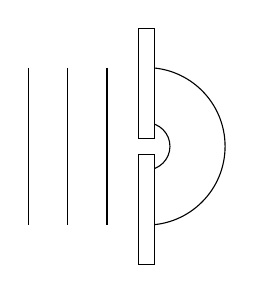
\begin{tikzpicture}
        \draw (-90:0.3) arc (-90:90:0.3);
        \draw (-90:1) arc (-90:90:1);
        \filldraw[color=black, fill=white] (-0.1, 0.1) rectangle (0.1, 1.5);
        \filldraw[color=black, fill=white] (-0.1, -0.1) rectangle (0.1, -1.5);
        \foreach \x in {-1.5, -1, -0.5} {\draw (\x, 1) -- (\x, -1);}
    \end{tikzpicture}
    \caption{波的衍射}
\end{figure}

\subsubsection{反射}

\begin{figure}[ht!]
    \centering
    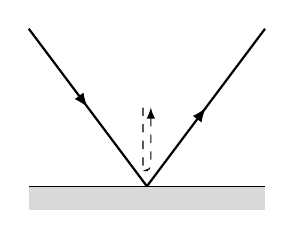
\begin{tikzpicture}
        \fill[fill=gray, opacity=0.3] (0,0) rectangle (3,-0.3);
        \draw (0,0) -- (3,0);
        \draw[thick, midarrow] (0,2) -- (1.5,0);
        \draw[thick, midarrow] (1.5,0) -- (3,2);
        \draw[dashed, rounded corners=2pt, -latex] (1.45,1) -- (1.45,0.2) -- (1.55,0.2) -- (1.55,1);
    \end{tikzpicture}
    \caption{波的反射}
\end{figure}
直观看来波在发生反射时遵循\underline{反射定律}\footnote{入射角=反射角},且整个过程中波的\underline{速度}、\underline{波长}、\underline{频率}不发生改变。但在介质层面则需要考虑反射端点类型的问题,一般分为以下两种:
\begin{itemize}
    \item 自由端:反射位置的介质可以自由移动的情况
    \item 固定端:反射位置的介质无法自由移动的情况
\end{itemize}
并通过假想一个不存在的波的方式处理各个时刻的反射波。
\begin{figure}[ht!]
    \centering
    \renewcommand\arraystretch{1.2}
    \begin{tabular}{c|cc}
        \hline
        反射端&反射波图示&反射波相变\\\hline
        自由端&镜面对称&0相变\\
        固定端&中心对称&$\pi$相变\\\hline
    \end{tabular}
    \caption{端点反射}
\end{figure}
\begin{figure}[ht!]
    \begin{minipage}[t]{0.48\textwidth}
        \centering
        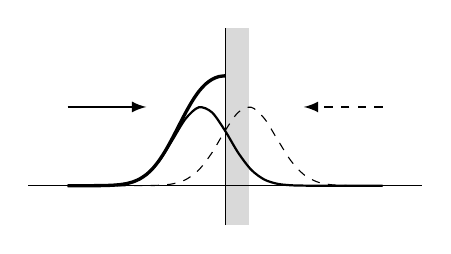
\begin{tikzpicture}
            \fill[fill=gray, opacity=0.3] (0,2) rectangle (0.3,-0.5);
            \draw (0,-0.5) -- (0,2);
            \draw (-2.5,0) -- (2.5,0);
            \draw[thick, domain=-2:2] plot[smooth] (\x, {exp(-4*(\x+0.3)^2)});
            \draw[dashed, domain=-2:2] plot[smooth] (\x, {exp(-4*(\x-0.3)^2)});
            \draw[very thick, domain=-2:0] plot[smooth] (\x, {exp(-4*(\x+0.3)^2)+exp(-4*(\x-0.3)^2)});
            \draw[thick, -latex] (-2,1) -- (-1,1);
            \draw[thick, dashed, -latex] (2,1) -- (1,1);
        \end{tikzpicture}
        \caption{自由端反射}
    \end{minipage}
    \begin{minipage}[t]{0.48\textwidth}
        \centering
        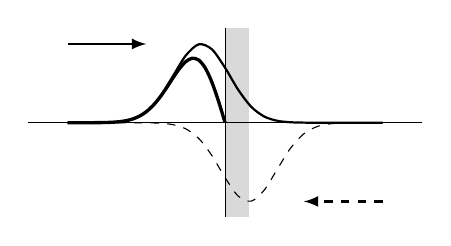
\begin{tikzpicture}
            \fill[fill=gray, opacity=0.3] (0,1.2) rectangle (0.3,-1.2);
            \draw (0,-1.2) -- (0,1.2);
            \draw (-2.5,0) -- (2.5,0);
            \draw[thick, domain=-2:2] plot[smooth] (\x, {exp(-4*(\x+0.3)^2)});
            \draw[dashed, domain=-2:2] plot[smooth] (\x, {-exp(-4*(\x-0.3)^2)});
            \draw[very thick, domain=-2:0] plot[smooth] (\x, {exp(-4*(\x+0.3)^2)-exp(-4*(\x-0.3)^2)});
            \draw[thick, -latex] (-2,1) -- (-1,1);
            \draw[thick, dashed, -latex] (2,-1) -- (1,-1);
        \end{tikzpicture}
        \caption{固定端反射}
    \end{minipage}
\end{figure}

\subsubsection{折射}

日文为屈折,内容较为基础,在此给出折射定律。
\begin{itembox}[l]{折射定律}
    \begin{equation*}
        \frac{\sin\theta_1}{\sin\theta_2}=
        \frac{v_1}{v_2}=
        \frac{\lambda_1}{\lambda_2}=
        \frac{n_2}{n_1}(=n_{12})
    \end{equation*}
\end{itembox}
需要注意公式中$n_{12}$的定义。此外,将折射角大于$90^\circ$的情况称为\underline{全反射},题目中一般考察临界入射角。

% chapter 3 section 2

\section{声波}

\subsection{声波}
\label{subsec:3.2.1}

\subsubsection{基本信息}

声波日文为音波,其基本内容与第一节相仿,在此仅逐条列举一些基本信息。
\begin{itemize}
    \item 介质:任何物体
    \item 本质:纵波
    \item 频率:20$\sim$20000Hz(人耳感知范围)
    \item 声速:空气中声速随温度改变:$v\approx331.5+0.6t$
    \item 三要素
    \begin{itemize}
        \item 音の高さ:取决于频率$f$
        \item 音色:取决于传递声音的介质
        \item 音の強さ:取决于$f^2A^2$,即日常使用的分贝(db, decibel)
    \end{itemize}
\end{itemize}

\subsubsection{差频}

日文为うなり,是两束频率相近的声波叠加时所发生的相互加强减弱的现象。其叠加而成的声波的频率满足以下公式。
\begin{itembox}[l]{差频公式}
    \begin{equation*}
        f=|f_1-f_2|
    \end{equation*}
\end{itembox}
\begin{figure}[ht!]
    \centering
    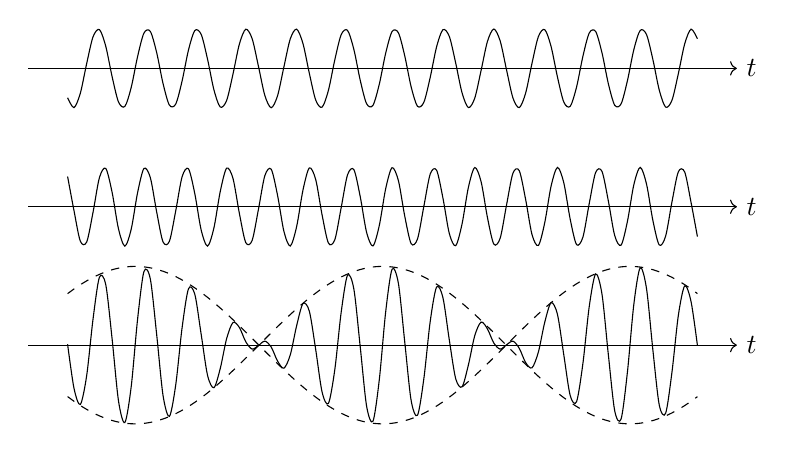
\begin{tikzpicture}
        \begin{scope}[yscale=0.5]
            \draw[->] (-4.5,0) -- (4.5,0) node[right] {$t$};
            \draw[domain=-4:4] plot[samples=100, smooth] (\x, {sin(10*\x r)});
        \end{scope}
        \begin{scope}[yscale=0.5, yshift=-100]
            \draw[->] (-4.5,0) -- (4.5,0) node[right] {$t$};
            \draw[domain=-4:4] plot[samples=100, smooth] (\x, {sin(12*\x r)});
        \end{scope}
        \begin{scope}[yscale=0.5, yshift=-200]
            \draw[->] (-4.5,0) -- (4.5,0) node[right] {$t$};
            \draw[domain=-4:4] plot[samples=100, smooth] (\x, {sin(10*\x r)+sin(12*\x r)});
            \draw[dashed, domain=-4:4] plot[samples=100, smooth] (\x, {2*cos(\x r)});
            \draw[dashed, domain=-4:4] plot[samples=100, smooth] (\x, {-2*cos(\x r)});
        \end{scope}
    \end{tikzpicture}
    \caption{差频}
\end{figure}
实际题目中常与下一小节的多普勒效应结合。

\subsection{多普勒效应}
\label{subsec:3.2.2}

日文为ドップラー効果,是观测者与波源存在相对运动时所发生的观测频率与波源频率不同的现象,日常生活中火车进站、警车鸣笛均属此类。根据观测者与波源的相对运动关系可分为以下三类。

\subsubsection{波源运动,观测者静止}

\begin{figure}[ht!]
    \centering
    \begin{tikzpicture}
        \clip (-3,-1.5) rectangle (3,1.5);
        \foreach \x/\r in {0/3, 0.2/2.5, 0.4/2, 0.6/1.5, 0.8/1} {
            \fill[opacity={\x+0.2}] (\x,0) circle (2pt);
            \draw[opacity={\x+0.2}] (\x,0) circle (\r);
        }
        \draw[thick, -latex] (0.4,0.5) -- (1,0.5);
    \end{tikzpicture}
    \caption{多普勒效应}
\end{figure}
由图可见,处于波源行进方向上的观测者会遇到更加密集的波面,反之则会遇到更加稀疏的波面。此所谓密集与稀疏实际指的是波面的间距,即波长。因此可以说波源的移动压缩/拉伸了波长。此时以波源为基准观察波速即为$V\pm v$。于是,根据波的基本公式可以得到以下结论。
\begin{equation*}
    V\pm v=f\lambda^\prime\implies
    \lambda^\prime=\frac{V\pm v}{f}
\end{equation*}
在观测者看来波仍然在以原速传播,所以观测者所感知到的频率即为
\begin{equation*}
    f^\prime=\frac{V}{\lambda^\prime}=\frac{V}{V\pm v}f
\end{equation*}

\subsubsection{波源静止,观测者运动}

此时,波源不移动,波长不发生改变。相当于观测者与各个波面在做追及+相遇,倘若两者相向而行,则单位时间内观测者会遇到更多的波面。反之则会遇到更少的波面。根据波的基本公式可以得到以下结论。
\begin{equation*}
    V\pm u=f^\prime\lambda\implies
    f^\prime=\frac{V\pm u}{\lambda}
    =\frac{V\pm u}{V}f
\end{equation*}

\subsubsection{波源运动,观测者运动}

基于上述两种情况的分析,我们可以把双方都运动的问题化简为运动的观测者感知波源压缩/拉伸后的波的问题。
\begin{itembox}[l]{多普勒效应}
    \begin{equation*}
        f^\prime=\frac{V\pm u}{V\pm v}f
    \end{equation*}
    \begin{itemize}
        \item V:波速
        \item u:观测者的速度
        \item v:波源的速度
    \end{itemize}
\end{itembox}
使用上述公式时应注意如下两点:
\begin{itemize}
    \item 观测者的速度和波源的速度的位置
    \item 分数中两个符号的判断\footnote{一般是结合推导过程记忆,但更推荐根据生活经验判断}
\end{itemize}
此外在实际题目中时而也会遇到一些其他变形。比如平面上的多普勒效应\footnote{基于运动的矢量性进行分解,只考虑发生多普勒效应的方向}、含有风的情况\footnote{风会带动介质运动,所以相当于改变了波速}等等。

\subsection{共振现象}
\label{subsec:3.2.3}

\paragraph{共振·共鸣}一般物体都具有一个固定的振动周期,当外界发生与之相同频率的变化时,该物体会受到其影响而发生距离振动的现象。当振动是以声音的形式展现时特称共鸣。

\subsubsection{弦振动}

拨动两端固定的弦,这个振动在弦上会以横波的形式向两端传播,到达端点后发生固定端反射,从而最终在弦上形成驻波。设弦的张力为$S$、线密度为$\rho$,则弦上波速可求。
\begin{figure}[ht!]
    \centering
    \begin{minipage}{0.48\textwidth}
        \begin{itembox}[l]{弦上波速}
            \begin{equation*}
                v=\sqrt{\frac{S}{\rho}}
            \end{equation*}
        \end{itembox}
        \begin{itembox}[l]{弦振动频率}
            \begin{itemize}
                \item $\lambda=\frac{2}{n}l$
                \item $f=\frac{nv}{2l}\implies nf_1=f_n$
            \end{itemize}
        \end{itembox}
    \end{minipage}
    \begin{minipage}{0.48\textwidth}
        \centering
        \begin{tikzpicture}
            \foreach \t/\yshift in {
                8/0, 4/-50, 2.67/-100, 2/-150
            } {
                \begin{scope}[yscale=0.8, yshift=\yshift]
                    \draw[color=gray] (0,0) -- (4,0);
                    \fill (0,0) circle (2pt);
                    \fill (4,0) circle (2pt);
                    \draw[domain=0:4] plot[samples=50, smooth] (\x, {0.5*sin((2*pi/\t)*(\x r)});
                    \draw[dashed, domain=0:4] plot[samples=50, smooth] (\x, {-0.5*sin((2*pi/\t)*(\x r)});
                \end{scope}
            }
        \end{tikzpicture}
        \caption{弦振动}
    \end{minipage}
\end{figure}
此外可以稳定形成驻波的振动均为弦的固有振动,其中我们将只有一个波峰的振动形式称为基本振动,称频率为基本振动频率n倍的振动形式为n倍振动。

\subsubsection{气柱振动}

与弦振动类似,通过吹气等方式使管内空气发生振动,同样也能形成驻波。当管口封闭时该端点形成固定端,反之形成自由端。我们将两端均开口的管称为开管,将一端开口、一端闭口的管称为闭管。分析其振动规律可得气柱振动的波长、频率等信息。此外对于闭管振动会出现开口端腹点(加强点)外移的现象\footnote{开口端补正:固定频率,改变管长,可由两次共振时的管长求得次偏移值。$\Delta x=\frac{l_2-3l_1}{2}$},但考试中鲜有提及,故此处略过。
\begin{figure}[ht!]
    \centering
    \begin{minipage}[t]{0.48\textwidth}
        \centering
        \begin{tikzpicture}
            \foreach \n/\t/\yshift in {
                1/8/0, 2/4/-50, 3/2.67/-100, 4/2/-150
            } {
                \begin{scope}[yscale=0.6, yshift=\yshift]
                    \node at (-1,0) {\n 倍振动};
                    \fill[fill=gray, opacity=0.2] (0,-0.6) rectangle (4,0.6);
                    \draw[thick] (0,0.6) -- (4,0.6);
                    \draw[thick] (0,-0.6) -- (4,-0.6);
                    \draw[domain=0:4] plot[samples=50, smooth] (\x, {0.5*cos((2*pi/\t)*(\x r)});
                    \draw[dashed, domain=0:4] plot[samples=50, smooth] (\x, {-0.5*cos((2*pi/\t)*(\x r)});
                \end{scope}
            }
        \end{tikzpicture}
        \caption{开管振动}
    \end{minipage}
    \begin{minipage}[t]{0.48\textwidth}
        \centering
        \begin{tikzpicture}
            \foreach \n/\t/\yshift in {
                1/16/0, 3/5.33/-50, 5/3.2/-100, 7/2.29/-150
            } {
                \begin{scope}[yscale=0.6, yshift=\yshift]
                    \node at (-1,0) {\n 倍振动};
                    \fill[fill=gray, opacity=0.2] (0,-0.6) rectangle (4,0.6);
                    \draw[thick] (4,-0.6) -- (0,-0.6) -- (0,0.6) -- (4,0.6);
                    \draw[domain=0:4] plot[samples=50, smooth] (\x, {0.5*sin((2*pi/\t)*(\x r)});
                    \draw[dashed, domain=0:4] plot[samples=50, smooth] (\x, {-0.5*sin((2*pi/\t)*(\x r)});
                \end{scope}
            }
        \end{tikzpicture}
        \caption{闭管振动}
    \end{minipage}
\end{figure}
\begin{itembox}[l]{气柱振动}
    \begin{itemize}
        \item 开管振动
        \begin{itemize}
            \item $\lambda=\frac{2}{n}l$
            \item $f=\frac{nv}{2l}\implies nf_1=f_n$
        \end{itemize}
        \item 闭管振动
        \begin{itemize}
            \item $\lambda=\frac{4}{2n-1}l$
            \item $f=\frac{(2n-1)v}{4l}\implies (2n-1)f_1=f_n$
        \end{itemize}
    \end{itemize}
\end{itembox}

% chapter 3 section 3

\section{光波}

光作为波的基本信息与第一节的内容相同,故在此略过,仅区分两个用语\footnote{为避免混淆,统一使用日语}。
\begin{itemize}
    \item 分散:虹、スペクトル(折射率不同导致)
    \item 散乱:青空、チンダル現象
\end{itemize}
其中分散现象由于折射率不同导致,体现光的波动性。而散乱现象主要体现光的粒子性,通俗地讲就是一些“跑偏”的光。

\subsection{光的折射}
\label{subsec:3.3.1}

\subsubsection{平行层}

由于$\sin\theta_in_i=const$,所以无论中间途径多少层不同的介质,最终的出射光线都会与入射光线平行。
\begin{figure}[ht!]
    \centering
    \begin{tikzpicture}
        \filldraw[color=black, fill=gray, fill opacity=0.3] (0,0) rectangle (4,0.5);
        \filldraw[color=black, fill=gray, fill opacity=0.8] (0,0.5) rectangle (4,1);
        \draw[thick, midarrow] (0.5,2) -- (1,1);
        \draw[thick, midarrow] (1,1) -- (2.3,0.5);
        \draw[thick, midarrow] (2.3,0.5) -- (3,0);
        \draw[thick, midarrow] (3,0) -- (3.5,-1);
    \end{tikzpicture}
    \caption{平行层折射}
\end{figure}

\subsubsection{水中视差}

从空气中观察水中物体,由于光的折射,实物总会比看起来的更深。其中实际深度$h$和视觉深度$h^\prime$满足$\frac{h}{n}=h^\prime$的关系。
\begin{figure}[ht!]
    \centering
    \begin{tikzpicture}[scale=1.5]
        \fill[fill=gray, opacity=0.3] (0,0) rectangle (3,-2);
        \draw (0,0) -- (3,0);
        
        \coordinate (A) at (1,0); \node[above] at (A) {$A$};
        \coordinate (B) at (2,0); \node[below right] at (B) {$B$};
        \coordinate (P) at (1,-1.8); \node[left] at (P) {$P$};
        \coordinate (PP) at (1,-1.2); \node[left] at (PP) {$P^\prime$};
        
        \fill (P) circle (2pt);

        \draw[thick, -latex] (P) -- (B) -- (3,1.2) node[right] {eye};
        \draw[thick, dashed] (PP) -- (B);
        \draw[thick, dashed] (A) -- (P);
        \draw[thick, dashed] (2,1) -- (2,-1);
        \drawangle[$\alpha$]{(B)}{(PP)}{(A)};
        \drawangle[$\beta$]{(B)}{(P)}{(A)};
        \drawangle[$\alpha$]{(3,1.2)}{(B)}{(2,1)};
        \drawangle[$\beta$]{(P)}{(B)}{(2,-1)};
    \end{tikzpicture}
    \caption{水中视差}
\end{figure}
\begin{equation*}
    AB=h^\prime\tan\alpha=h\tan\beta
    \xrightarrow[\tan\approx\sin]{\sin\alpha=\sin\beta n}
    h^\prime=\frac{h}{n}
\end{equation*}

\subsubsection{透镜}

当给定透镜的部分定量信息后,通过透镜公式便可以其他相关定量信息。
\begin{itembox}[l]{透镜公式}
    \begin{equation*}
        \frac{1}{a}+\frac{1}{b}=\frac{1}{f}
    \end{equation*}
    \begin{itemize}
        \item 参数:
        \begin{center}
            \renewcommand\arraystretch{1.2}
            \begin{tabular}{c|cc}
                \hline
                参数&正数&负数\\\hline
                焦距f&凸透镜&凹透镜\\
                物距a&实物&虚物\\
                相距b&实相&虚像\\\hline
            \end{tabular}
        \end{center}
        \item 倍率:$m=\left\lvert\frac{b}{a}\right\rvert$
    \end{itemize}
\end{itembox}

\subsection{光的干涉}
l\label{subsec:3.3.2}

\subsubsection{双缝干涉}

\paragraph{实验内容}双缝实验是英国科学家托马斯杨于1807年为了验证光的波动性所做的实验。从光源$S_0$发出的单色光,通过双缝$S_1$和$S_2$投射到光屏上,其中相比于双缝的间距$d$,光屏的距离$l$足够远。实验发现光屏上会呈现出明暗相间的条纹。
\begin{figure}[ht!]
    \centering
    \begin{tikzpicture}[scale=1.5]
        \draw[thick] (-0.5,0.3) -- (-0.5,-0.3);
        \draw[thick] (0,1) -- (0,0.55);
        \draw[thick] (0,0.45) -- (0,-0.45);
        \draw[thick] (0,-0.55) -- (0,-1);
        \draw (0,0) -- (3.5,0);
        \draw (3,-1) -- (3,1) -- (3.5,1);
        \draw[<->] (3.4,0) -- node[fill=white] {$x$} (3.4,1);

        \coordinate (S0) at (-0.5,0); \node[left] at (S0) {$S_0$};
        \coordinate (S1) at (0,0.5); \node[above left] at (S1) {$S_1$};
        \coordinate (S2) at (0,-0.5); \node[below left] at (S2) {$S_2$};
        \coordinate (H) at (0.4,-0.3); \node[below] at (H) {$H$};
        \coordinate (P) at (3,1); \node[above] at (P) {$P$};

        \draw[dashed] (S1) -- (-1.5,0.5);
        \draw[dashed] (S2) -- (-1.5,-0.5);
        \draw[<->] (-1.4,0.5) -- node[fill=white] {$d$} (-1.4,-0.5);
        \draw[<->] (0,-0.8) -- node[fill=white] {$l$} (3,-0.8);
        \draw[midarrow] (S0) -- (S1) -- (P);
        \draw[midarrow] (S0) -- (S2) -- (P);
        \draw[dashed] (0,0) -- (P);
        \draw[dashed] (0,0.5) -- (H);
        \drawangle[]{(S2)}{(S1)}{(H)};
        \drawangle{(3,0)}{(0,0)}{(P)};
    \end{tikzpicture}
    \caption{双缝干涉}
\end{figure}

\paragraph{干涉条件}根据图形关系可知,两束光线到达$P$点距离的差值为$|S_1P-S_2P|=\frac{dx}{l}$,再结合平面波干涉的结论可得双缝干涉条件。
\begin{itembox}[l]{双缝干涉条件}
    \begin{equation*}
        \frac{dx}{l}=
        \begin{cases}
            2m\cdot\frac{\lambda}{2}&\implies\textrm{明线}\\
            (2m+1)\cdot\frac{\lambda}{2}&\implies\textrm{暗线}
        \end{cases}
    \end{equation*}
\end{itembox}

\paragraph{条纹间距}基于相邻两次干涉位置可求双缝干涉的条纹间距。
\begin{equation*}
    \Delta x=x_m-x_{m-1}=\frac{l\lambda}{d}
\end{equation*}
因此,若是知道$l$,$d$,$\Delta x$的信息即可反向求出波长。

\paragraph{颜色变化}另外,如果光源发出的是全色光则会发现$x=0$的位置出现白色条纹,其两侧由紫色向红色渐变展开。因为对于所有颜色的光$x=0$的位置永远是第零次加强的位置,所以全部汇聚于此,呈现白色。再根据条纹间距可知,波长较短的紫色会离其第零次干涉位置更近,所以白色旁边先会出现紫色。

\paragraph{回折格子}即布满等距缝隙的薄片,其实验原理与双缝干涉一致,只是同时相互干涉的光线更多。因此,不同于双缝干涉,回折格子的明线会更加明显。在此只给出结论。
\begin{itembox}[l]{回折格子干涉条件}
    \begin{equation*}
        d\sin\theta=m\lambda
    \end{equation*}
\end{itembox}

\subsubsection{薄膜干涉}

\paragraph{反射相变}光波在发生反射时根据接触面光学性质的不同会发生位相的变化。在此将折射率大的介质称为\underline{光密},相反称折射率小的介质称为\underline{光疏}。
\begin{figure}[ht!]
    \centering
    \renewcommand\arraystretch{1.2}
    \begin{tabular}{c|cc}
        \hline
        反射&反射端&相变\\\hline
        光密$\to$光疏&自由端&0相变\\
        光疏$\to$光密&固定端&$\pi$相变\\\hline
    \end{tabular}
    \caption{反射相变}
\end{figure}

\paragraph{光程}日文为光学距離,指在统一相位变化的前提下描述光波走行距离的量,并且简称光程相等的两条路径\underline{等光程}。我们在所有干涉实验中着眼的便是这个物理量。
\begin{figure}[ht!]
    \centering
    \begin{tikzpicture}
        \foreach \n [count=\i] in {1.5, 2} {
            \begin{scope}[yscale=0.5, yshift={-100*(\i-1)}]
                \draw (-2.5,0) -- (5,0);
                \filldraw[color=black, fill=gray, fill opacity={0.3*\i}] (0,-1) rectangle ({4/\n},1);
                \draw[domain=-2:0] plot[samples=50] (\x, {sin((pi*\x) r)});
                \draw[domain=0:{4/\n}] plot[samples=50] (\x, {sin((\n*pi*\x) r)});
                \draw[domain={4/\n}:4.5] plot[samples=50] (\x, {sin((pi*(\x-4/\n)) r)});
                \draw[<->] (0,1.2) -- node[above] {$l_\i$} ({4/\n},1.2);
            \end{scope}
        }
    \end{tikzpicture}
    \caption{光程}
\end{figure}
\begin{itembox}[l]{光程公式}
    \begin{equation*}
        L=nl
    \end{equation*}
\end{itembox}

\paragraph{实验内容}空间中有一层薄膜,光波斜向而来,观察在膜的表面与底层发生反射的两束光线。实验发现,在膜的表面会出现明暗相间的干涉条纹。
\begin{figure}[ht!]
    \centering
    \begin{tikzpicture}[scale=0.8]
        \fill[fill=gray, opacity=0.3] (0,0) rectangle (6,-2);
        \draw (0,0) -- (6,0);
        \draw (0,-2) -- (6,-2);

        \draw[thick, midarrow] (1,1) -- (2,0);
        \draw[thick, midarrow] (2,2) -- (4,0);
        \draw[thick, -latex] (4,0) -- (5,1);
        \draw[thick] (2,0) -- (3,-2) -- (4,0);

        \node[below left] at (2,0) {$A$};
        \node[below right] at (4,0) {$B$};
        \node[below left] at (3,-2) {$C$};
        \node[right] at (4,-4) {$C^\prime$};
        \node[above right] at (3,1) {$D$};
        \node[right] at (2.4,-0.8) {$H$};

        \draw[dashed] (2,-1) -- (2,1);
        \draw[dashed] (2,0) -- (3,1);
        \draw[dashed] (2.4,-0.8) -- (4,0) -- (4,-4) -- (3,-2);
        \draw[dashed, <->] (0.1,0) -- node[right] {$d$} (0.1,-2);

        \drawangle[$\theta$]{(2,1)}{(2,0)}{(1,1)};
        \drawangle[$\phi$]{(2,-1)}{(2,0)}{(3,-2)};
    \end{tikzpicture}
    \caption{薄膜干涉}
\end{figure}

\paragraph{干涉条件}根据图形关系可知,两束光线在B点处的光程差为$2nd\cos\phi$。因此,结合反射相变可得如下干涉条件。
\begin{itembox}[l]{薄膜干涉条件}
    \begin{equation*}
        2nd\cos\phi=
        \begin{cases}
            2m\cdot\frac{\lambda}{2}&\implies
            \textrm{0相变明线/}\pi\textrm{相变暗线}\\
            (2m+1)\cdot\frac{\lambda}{2}&\implies
            \textrm{0相变暗线/}\pi\textrm{相变明线}
        \end{cases}
    \end{equation*}
\end{itembox}

\subsubsection{楔形膜干涉}

\paragraph{实验内容}空间中有两块以极小夹角叠放的玻璃砖,光线从其上方垂直而来,观察在上玻璃砖的底面与下玻璃砖的顶面发生反射的两束光线。实验发现,在上玻璃砖的表面会出现明暗相间的干涉条纹。
\begin{figure}[ht!]
    \centering
    \begin{tikzpicture}
        \draw (0,0) rectangle (3,-0.5);
        \draw[rotate=15] (0,0) rectangle (3,0.5);

        \draw[thick, -latex, rounded corners=2pt] ($(15:2)+(0,1)$) -- (15:2) -- (15:1.9) -- ($(15:1.9)+(0,1)$);
        \draw[thick, -latex, rounded corners=2pt] ($(15:2.1)+(0,1)$) -- (0:2) -- (0:2.1) -- ($(15:2.2)+(0,1)$);

        \drawangle{(0:3)}{(0,0)}{(15:3)};
        \draw[<->] (0,-0.1) -- node[below] {$x$} (2.1,-0.1);
        \draw[<->] (14:2.3) -- node[right] {$d$} (0:2.2);
    \end{tikzpicture}
    \caption{楔形膜干涉}
\end{figure}

\paragraph{干涉条件}根据图形关系不难发现两束光线的光程差为$2d$,一般夹角$\theta$为给定值,所以光程差也可以用$2x\tan\theta$表示。再结合反射相变可得如下干涉条件。
\begin{itembox}[l]{楔形膜干涉条件}
    \begin{equation*}
        2d=2x\tan\theta=
        \begin{cases}
            2m\cdot\frac{\lambda}{2}&\implies
            \textrm{0相变明线/}\pi\textrm{相变暗线}\\
            (2m+1)\cdot\frac{\lambda}{2}&\implies
            \textrm{0相变暗线/}\pi\textrm{相变明线}
        \end{cases}
    \end{equation*}
\end{itembox}

\paragraph{条纹间距}与双缝干涉条纹间距求解思路一致,楔形膜干涉中同种干涉条纹间距为
\begin{equation*}
    \Delta x=x_m-x_{m-1}=\frac{\lambda}{2\tan\theta}
\end{equation*}

\subsubsection{牛顿环干涉}

\paragraph{实验内容}在空间中有一块半径足够大的平凸透镜凸面朝下放在一块玻璃砖上,光线从其上方垂直而来,观察在平凸透镜的底面与玻璃砖的顶面发生反射的两束光线。实验发现,在平凸透镜表面会出现明暗相间的圆环状干涉条纹。
\begin{figure}[ht!]
    \centering
    \begin{tikzpicture}
        \filldraw[color=black, fill=gray, fill opacity=0.3] (-120:4) arc (-120:-60:4) --cycle;
        \filldraw[color=black, fill=gray, fill opacity=0.3] (-2,-4) rectangle (2,-4.5);

        \fill (0,0) circle (1.5pt);
        \draw[dashed] (0,0) -- (0,-4.7);
        \draw[dashed] (1.37,-3.76) -- (1.37,-4.7);
        \draw[<->] (0,-4.6) -- node[below] {$r$} (1.37,-4.6);
        \draw[dashed] (0,0) -- node[left] {$R$} (-70:4);
        \node at (2,-3.7) {$d$};

        \draw[thick, -latex, rounded corners=2pt] (1.37,-2) -- (-70:4) -- (1.27,-3.76) -- (1.27,-2);
        \draw[thick, -latex, rounded corners=2pt] (1.47,-2) -- (1.47,-4) -- (1.57,-4) -- (1.57,-2);
    \end{tikzpicture}
    \caption{牛顿环干涉}
\end{figure}

\paragraph{干涉条件}根据图形关系可得两束光线的光程差为$2d$,使用凸透镜半径$R$和干涉点到圆心距离$r$后可表示为$\frac{r^2}{R}$,结合反射相变可得如下干涉条件。
\begin{itembox}[l]{牛顿环干涉条件}
    \begin{equation*}
        2d=\frac{r^2}{R}=
        \begin{cases}
            2m\cdot\frac{\lambda}{2}&\implies
            \textrm{0相变明线/}\pi\textrm{相变暗线}\\
            (2m+1)\cdot\frac{\lambda}{2}&\implies
            \textrm{0相变暗线/}\pi\textrm{相变明线}
        \end{cases}
    \end{equation*}
\end{itembox}


    % chapter 4

\chapter{电磁}

% chapter 4 section 1

\section{电场}

\subsection{电场}
\label{subsec:电场}

\subsubsection{电荷}

物体的带电量称为电荷,日文中也可用電気量一词。其单位为库伦(C),且带电体间时常有满足库仑定律\footnote{诱电率$\varepsilon=\frac{1}{4k\pi}$}的作用力存在。
\begin{itembox}[l]{库仑定律}
    \begin{equation*}
        F=k\frac{Qq}{r^2}
    \end{equation*}
    \begin{itemize}
        \item $k=9\times10^9N\cdot m^2\cdot C^{-2}$
        \item 同性相斥,异性相吸
    \end{itemize}
\end{itembox}

\subsubsection{电场}

为了更方便得解释诸如重力、万有引力、电磁力等非接触力的作用方式,人们引入了“场” 的概念,并认为是场传递了各种各样的物理信息。因此在空间中传递上述库仑力的场即为\underline{电场},用单位电荷的受力定义。

\begin{figure}[p!]
    \centering
    \begin{minipage}[t]{0.48\textwidth}
        \centering
        \begin{tikzpicture}[scale=0.5]
            \node[draw, circle] at (0,0) {$+$};
            \foreach \x in {-3,...,3} \foreach \y in {-3,...,3} {
                \pgfmathparse{and(equal(\x,0),equal(\y,0))}
                \ifnum\pgfmathresult=1
                \else
                \draw[-stealth, opacity={1/sqrt((\x)^2+(\y)^2)}] (\x,\y) -- ++ (
                    {0.5*\x/sqrt((\x)^2+(\y)^2)},
                    {0.5*\y/sqrt((\x)^2+(\y)^2)}
                );
                \fi
            }
        \end{tikzpicture}
        \caption{单正点电荷电场图示}
    \end{minipage}
    \begin{minipage}[t]{0.48\textwidth}
        \centering
        \begin{tikzpicture}[scale=0.5]
            \node[draw, circle] at (0,0) {$-$};
            \foreach \x in {-3,...,3} \foreach \y in {-3,...,3} {
                \pgfmathparse{and(equal(\x,0),equal(\y,0))}
                \ifnum\pgfmathresult=1
                \else
                \draw[-stealth, opacity={1/sqrt((\x)^2+(\y)^2)}] ($(\x,\y)+(
                    {0.5*\x/sqrt((\x)^2+(\y)^2)},
                    {0.5*\y/sqrt((\x)^2+(\y)^2)}
                )$) -- (\x,\y);
                \fi
            }
        \end{tikzpicture}
        \caption{单负点电荷电场图示}
    \end{minipage}
\end{figure}

\begin{figure}[p!]
    \centering
    \begin{tikzpicture}[scale=0.5]
        \node[draw, circle] at (-4,0) {$+$};
        \node[draw, circle] at (4,0) {$-$};
        \foreach \x in {-8,...,8} \foreach \y in {-4,...,4} {
            \pgfmathparse{or(
                and(equal(\x,-4),equal(\y,0)),
                and(equal(\x,4),equal(\y,0))
            )}
            \ifnum\pgfmathresult=1
            \else
            \draw[-stealth] (\x,\y) -- ++ (
                {0.3*((\x+4)/sqrt((\x+4)^2+(\y)^2)-(\x-4)/sqrt((\x-4)^2+(\y)^2))},
                {0.3*(\y/sqrt((\x+4)^2+(\y)^2)-\y/sqrt((\x-4)^2+(\y)^2))}
            );
            \fi
        }
    \end{tikzpicture}
    \caption{正-负点电荷电场图示}
\end{figure}

\begin{figure}[p!]
    \centering
    \begin{tikzpicture}[scale=0.5]
        \node[draw, circle] at (-4,0) {$+$};
        \node[draw, circle] at (4,0) {$+$};
        \foreach \x in {-8,...,8} \foreach \y in {-4,...,4} {
            \pgfmathparse{or(
                and(equal(\x,-4),equal(\y,0)),
                and(equal(\x,4),equal(\y,0))
            )}
            \ifnum\pgfmathresult=1
            \else
            \draw[-stealth] (\x,\y) -- ++ (
                {0.3*((\x+4)/sqrt((\x+4)^2+(\y)^2)+(\x-4)/sqrt((\x-4)^2+(\y)^2))},
                {0.3*(\y/sqrt((\x+4)^2+(\y)^2)+\y/sqrt((\x-4)^2+(\y)^2))}
            );
            \fi
        }
    \end{tikzpicture}
    \caption{正-正点电荷电场图示}
\end{figure}

\begin{itembox}[l]{电场}
    \begin{equation*}
        \vec{E}=\frac{\vec{F}}{q}
        \iff
        \vec{F}=q\vec{E}
    \end{equation*}
    \begin{itemize}
        \item 单位:N/C
        \item 点电荷周围的电场:$E=k\frac{Q}{r^2}$
    \end{itemize}
\end{itembox}
根据定义可知电场也是一个矢量,所以在实际运用过程中也满足矢量的合成与分解。

\subsection{电势}
\label{subsec:电势}

\subsubsection{电势能与电势}

观察库仑力形式可发现其与万有引力十分相像,因此不难推测库仑力也是保存力。因而也有其对应的势能,即\underline{电势能},日文为静電気力による位置エネルギー。

此外,为了描述物理现象与计算使用方便,人们也引入了电场中单位电荷的电势能:电势(日文为電位)这个物理量,单位为伏特(V)。因此,电势能与电势之间满足如下关系。
\begin{itembox}[l]{电势能与电势}
    \begin{equation*}
        U=qV
    \end{equation*}
\end{itembox}

\subsubsection{典型电场中的电势}

\paragraph{匀强电场的电势}日文为一様電場,即大小、方向均衡定的电场。
\begin{figure}[ht!]
    \centering
    \begin{tikzpicture}
        \foreach \y in {0,1,2} {\draw[opacity=0.3, -latex] (4,\y) -- (0,\y);}
        \fill (0.5,1) circle (2pt) node[below] {$O$};
        \fill (1.5,1) circle (2pt) node[below] {$B$};
        \fill (3.5,1) circle (2pt) node[below] {$A$};
        \draw[<->] (1.5,1.3) -- node[fill=white] {$d$} (3.5,1.3);
    \end{tikzpicture}
    \caption{匀强电场电势}
\end{figure}
那么,匀强电场中倘若某两点间距为$d$,期间将会存在
\begin{equation*}
    V=\frac{Eq\times d}{q}=Ed
\end{equation*}
大小的电势,并称其为该两点间的\underline{电势差}。

\paragraph{点电荷电场的电势}

规定离场源电荷无限远处为电势基准,则可得点电荷周围电势公式。
\begin{itembox}[l]{点电荷电势}
    \begin{equation*}
        V=k\frac{Q}{r}
    \end{equation*}
\end{itembox}

\subsubsection{等电势面}

类比于地图上描述地势分布的等高线,等电势线/面也常常用于描述电势的分布,且具有如下性质。
\begin{itemize}
    \item 与电场线垂直
    \item 等电位面密$\iff$电场线密$\iff$电场强
\end{itemize}
\begin{figure}[ht!]
    \centering
    \begin{tikzpicture}[scale=0.6]
        \foreach \r in {1,...,3} {\draw[opacity={1/\r}] (0,0) circle (\r);}
        \foreach \a in {1,...,12} {\draw[thick, -latex] (0,0) -- ({\a*30}:3.5);}
        \node[circle, fill=white] at (0,0) {$+$};
    \end{tikzpicture}
    \caption{等电势面}
\end{figure}

\subsubsection{总结}

鉴于本节内容较多且不易梳理清晰,特此简做总结。
\begin{figure}[ht!]
    \centering
    \renewcommand\arraystretch{1.5}
    \begin{tabular}{c|c|c|c|c}
        \hline
        &电场E&库仑力F&电势能U&电势V\\\hline
        重力场&$g$&$mg$&$mgh$&$gh$\\\hline
        点电荷&$\frac{kQ}{r^2}$&$\frac{kQq}{r^2}$&$\frac{kQq}{r}$&$\frac{kQ}{r}$\\\hline
    \end{tabular}
    \caption{电场电势总结}
\end{figure}

\subsection{电容器}
\label{subsec:电容器}

\subsubsection{基本原理}

电容器,日文为コンデンサー,是电路中基本的储能元件,其符号如图。
\begin{figure}[ht!]
    \centering
    \begin{circuitikz}
        \draw (0,0) to[C=$3\mu F$,o-o] (2,0);
    \end{circuitikz}
\end{figure}
就比较简单的平行板电容器而言,其基本工作原理为:极板两端由于电势高低不同因而汇聚正负电荷,异种电荷相互吸引从而不断增大极板两端的电势差,直到与外路相同为止。在这个过程中电容器所“收集”的电荷量可由电容器定义式得来。
\begin{itembox}[l]{电容器定义式}
    \begin{equation*}
        Q=CV
    \end{equation*}
    \begin{itemize}
        \item V:极板两端的电势差
        \item C:电容量,日文为電気容量,单位为法拉(F)
    \end{itemize}
\end{itembox}

\begin{itembox}[l]{平行板电容器}
    \begin{equation*}
        C=\varepsilon_0\frac{S}{d}
    \end{equation*}
    \begin{itemize}
        \item $\varepsilon_0$:绝对诱电率
        \item 极板间电场:$E=\frac{V}{d}=\frac{Q}{\varepsilon_0S}$
    \end{itemize}
\end{itembox}

\subsubsection{电容器串并联}

\begin{figure}[ht!]
    \centering
    \begin{minipage}{0.48\textwidth}
        \begin{itembox}[l]{串联}
            \begin{itemize}
                \item 电荷相等
                \item $\frac{Q}{C_1}+\frac{Q}{C_2}=V$
                \item $\frac{Q}{C}=V$
                \item $\frac{1}{C}=\frac{1}{C_1}+\frac{1}{C_2}$
            \end{itemize}
        \end{itembox}
    \end{minipage}
    \begin{minipage}{0.48\textwidth}
        \centering
        \begin{circuitikz}[european]
            \draw (0,0)
            to[battery1, invert] (0,2)
            to[short] (2,2)
            to[C=$C_1$] (2,1)
            to[C=$C_2$] (2,0)
            to[short] (0,0);
        \end{circuitikz}
        \caption{电容器串联}
    \end{minipage}
\end{figure}

\begin{figure}[ht!]
    \centering
    \begin{minipage}{0.48\textwidth}
        \begin{itembox}[l]{并联}
            \begin{itemize}
                \item 电压相等
                \item $VC_1+VC_2=Q$
                \item $VC=Q$
                \item $C=C_1+C_2$
            \end{itemize}
        \end{itembox}
    \end{minipage}
    \begin{minipage}{0.48\textwidth}
        \centering
        \begin{circuitikz}[european]
            \draw (0,0)
            to[battery1, invert] (0,2)
            to[short] (1.5,2)
            to[C=$C_1$] (1.5,0)
            to[short] (0,0);
            \draw (1.5,2)
            to[short] (3,2)
            to[C=$C_2$] (3,0)
            to[short] (1.5,0);
        \end{circuitikz}
        \caption{电容器并联}
    \end{minipage}
\end{figure}

\subsubsection{电容器储能}

\paragraph{储能}电容器在充电(积攒能量)的过程中,电荷量与电势差共同增长。根据电势能公式,在电势差为V的某个时刻汇聚过来的电荷q会携带$U=qV$大小的能量。将整个过程绘制成$Q-V$图像,那么总能量即为图中三角形的面积。
\begin{figure}[ht!]
    \centering
    \begin{tikzpicture}
        \draw[->] (0,0) -- (2,0) node[right] {Q};
        \draw[->] (0,0) -- (0,2) node[above] {V};
        \filldraw[color=black, fill=gray, fill opacity=0.3] (0,0) -- (1.5,1.5) -- (1.5,0) -- cycle;
        \node at (1,0.5) {U};
    \end{tikzpicture}
    \caption{电容器储能}
\end{figure}
\begin{itembox}[l]{电容器储能}
    \begin{equation*}
        U=\frac12QV=\frac12CV^2=\frac{Q^2}{2C}
    \end{equation*}
\end{itembox}

此外,假设与电容器串联的外路的总电阻为$R$,那么根据基尔霍夫定律可得
\begin{gather*}
    E=IR+\frac{Q}{C}\\
    I=\frac{E-\frac{Q}{C}}{R}
\end{gather*}
当电路接通的瞬间,电容器不带电($Q=0$),所以回路电流为$I=\frac{E}{R}$。如此一来则可以粗略地认为此时电容器就是一根导线。
\begin{figure}[ht!]
    \centering
    \begin{minipage}{0.48\textwidth}
        \centering
        \begin{tikzpicture}
            \draw[->] (0,0) -- (4,0) node[right] {$t$};
            \draw[->] (0,-1.5) -- (0,1.5) node[above] {$I$};
            \draw[thick] (0,0) -- (0.5,0) -- (0.5,1);
            \draw[thick, domain=0.5:2.5] plot[smooth] (\x, {exp(2-4*\x)});
            \draw[thick] (2.5,0) -- (2.5,-1);
            \draw[thick, domain=2.5:4] plot[smooth] (\x, {-exp(10-4*\x)});
        \end{tikzpicture}
    \end{minipage}
    \begin{minipage}{0.48\textwidth}
        \centering
        \begin{tikzpicture}
            \draw[->] (0,0) -- (4,0) node[right] {$t$};
            \draw[->] (0,-1.5) -- (0,1.5) node[above] {$V$};
            \draw[thick] (0,0) -- (0.5,0);
            \draw[thick, domain=0.5:2.5] plot[smooth] (\x, {1-exp(2-4*\x)});
            \draw[thick, domain=2.5:4] plot[smooth] (\x, {exp(10-4*\x)});
        \end{tikzpicture}
    \end{minipage}
    \caption{电容器储能时IV变化}
\end{figure}

\paragraph{损耗}在给电容器充电的过程中,电源做功\footnote{给$Q$大小的电荷提供了$V$大小的电压,使其获得了$QV$大小的电势能}为$W=QV$。根据能量守恒定律可知,其中有
\begin{equation*}
    W-U=QV-\frac12QV=\frac12QV
\end{equation*}
大小的能量在途中损耗了。由于整个过程中没有其他能量形式,因此可知整个充电过程中产生了$\frac12QV$大小的焦耳热。

\subsubsection{极板间引力}

结合带电体在电场中的受力可知,平行板电容器的极板间存在相互吸引的力。其间的电场为$E=E_\textrm{上}+E_\textrm{下}$,因为上下极板带电量相等,所以产生的场强也相等。着眼于上极板吸引下极板的部分可得
\begin{itembox}[l]{极板间引力}
    \begin{equation*}
        F=QE_\textrm{上}=\frac12QE
    \end{equation*}
\end{itembox}

\subsubsection{平行板电容器改装}

\begin{figure}[ht!]
    \centering
    \begin{minipage}[t]{0.48\textwidth}
        \centering
        \begin{tikzpicture}[yscale=0.6]
            \foreach \y in {0,1,2} {\draw[thick, -latex] (0,\y) -- (3,\y);}
            \filldraw[color=black, fill=gray!30] (0.5,-0.2) rectangle (2.5,2.2);
            \node at (1.5,1) {$E=0$};
        \end{tikzpicture}
        \caption{静电屏蔽}
    \end{minipage}
    \begin{minipage}[t]{0.48\textwidth}
        \centering
        \begin{tikzpicture}[yscale=0.6]
            \foreach \y in {0,1,2} {\draw[thick, -latex] (0,\y) -- (3,\y);}
            \filldraw[color=black, fill=gray!30] (0.5,-0.2) rectangle (2.5,2.2);
            \foreach \y in {0.5,1.5} {\draw[-latex] (0.5,\y) -- (2.5,\y);}
            \node at (1.5,1) {$E=E_0/\varepsilon_r$};
        \end{tikzpicture}
        \caption{电极化}
    \end{minipage}
\end{figure}

\paragraph{静电屏蔽}日文为静電遮蔽。将导体放入电场后,导体中的电子受电场力影响汇聚到导体两端,形成抵消外部电场的电场。

\paragraph{电极化}日文为誘電分極。将绝缘体放入电场后,由于内部电子无法自由移动,只能发生小范围偏移,因而无法完全抵消外部电场。所以在日文中绝缘体也可称作誘電体。

\begin{figure}[ht!]
    \centering
    \begin{tikzpicture}
        \draw[thick] (0,0) -- (0.5,0);
        \draw[thick] (2.5,0) -- (3,0);
        \draw[thick] (0.5,0.5) -- (0.5,-0.5);
        \draw[thick] (2.5,0.5) -- (2.5,-0.5);
        \fill[fill=gray!30] (1.2,-0.5) rectangle (2.2,0.5);
        
        \draw[<->] (1.2,0.7) -- node[above] {l} (2.2,0.7);
        \draw[<->] (0.5,-0.7) -- node[below] {d} (2.5,-0.7);
    \end{tikzpicture}
    \caption{电容器改装}
\end{figure}

\paragraph{导体改装}根据静电屏蔽现象可知导体块内无电场,因此没有电势降落,所以可以视其为一段导线。现假设插入的导体块与左极板的距离为x,则根据电容器串联公式可得
\begin{gather*}
    \frac{1}{C}=\frac{1}{\varepsilon_0\frac{S}{x}}+\frac{1}{\varepsilon_0\frac{S}{d-l-x}}\\
    C=\varepsilon_0\frac{S}{d-l}
\end{gather*}

\paragraph{绝缘体改装}主体思路与导体改装一致:将改装后的电容器视作多个电容器串联。在此只补充含绝缘体部分的电容量的变化
\begin{gather*}
    E^\prime=\frac{E}{\varepsilon_r}\implies
    V^\prime=\frac{V}{\varepsilon_r}\\
    Q=CV=C^\prime V^\prime\\
    C^\prime=\varepsilon_rC
\end{gather*}

\paragraph{复杂改装}时而题目中也会出现插入的物体不足以覆盖整个极板的情况,此时只需将已覆盖的部分与未覆盖的部分看作两个电容器并联处理即可。

% chapter 4 section 2

\section{电流}

\subsection{欧姆定律}

本节内容较为基础,在此只逐条列举重要知识点。

\subsubsection{电流}

\begin{itemize}
    \item 描述:由电荷的定向移动形成
    \item 方向:正电荷的流动方向,或者负电荷流动的反方向
    \item 大小:单位时间内流过导体截面的电量
    \item 定义式1(宏观):
    \begin{equation*}
        I=\frac{\Delta Q}{\Delta t}
    \end{equation*}
    \item 定义式2(微观)\footnote{n为单位体积的电子密度,v为电子移动速度,S为导体截面积}:
    \begin{equation*}
        I=neSv
    \end{equation*}
    \item 单位:安培(A)
\end{itemize}

\subsubsection{欧姆定律}

\begin{equation*}
    V=IR
\end{equation*}
\begin{itemize}
    \item 描述:流过导体的电流与加在其两端电压的大小成正比
    \item 电阻R:日文为電気抵抗
    \begin{itemize}
        \item 单位:欧姆($\Omega$)
        \item 定义式:$R=\rho\frac{l}{S}$
    \end{itemize}
\end{itemize}

\subsubsection{焦耳热}

\begin{itemize}
    \item 本质:电场力对电子的做功
    \item 公式:
    \begin{equation*}
        Q=VIt=I^2Rt=\frac{V^2}{R}t
    \end{equation*}
    \item (电)功率:
    \begin{equation*}
        W=VI=I^2R=\frac{V^2}{R}
    \end{equation*}
\end{itemize}

\subsection{直流电路}

\textbackslash\textbackslash TODO

% chapter 4 section 3

\section{磁场}

\subsection{磁场}

\subsubsection{电与磁}

磁的体系与电十分类似,几乎所有磁的概念\footnote{磁场中不存在独立的单极磁荷}都可以在电中找到对应的内容。
\begin{figure}[ht!]
    \centering
    \renewcommand\arraystretch{1.2}
    \begin{tabular}{c|c|c}
        \hline
        &电&磁\\\hline
        基本单位&电荷C&磁荷Wb\\\hline
        场力&电场力(库仑力)&磁场力\\\hline
        场常数&电容率$\varepsilon$(誘電率)&磁导率$\mu$(透磁率)\\\hline
    \end{tabular}
    \caption{电与磁对比}
\end{figure}

因此,磁场的直觉定义即为
\begin{equation*}
    \vec{H}=\frac{\vec{F}}{m}\quad(N/Wb)
\end{equation*}
同样也存在描述磁场走势、大小等信息的磁场线,并具有以下性质。
\begin{itemize}
    \item N极出,S极入
    \item 磁场线密$\iff$磁场强
\end{itemize}
\begin{figure}[ht!]
    \centering
    \begin{tikzpicture}[scale=0.45]
        \foreach \x in {-8,...,8} \foreach \y in {-4,...,4} {
            \pgfmathparse{or(
                and(equal(\x,-4),equal(\y,0)),
                and(equal(\x,4),equal(\y,0))
            )}
            \ifnum\pgfmathresult=1
            \else
            \draw[-stealth] (\x,\y) -- ++ (
                {0.3*((\x+4)/sqrt((\x+4)^2+(\y)^2)-(\x-4)/sqrt((\x-4)^2+(\y)^2))},
                {0.3*(\y/sqrt((\x+4)^2+(\y)^2)-\y/sqrt((\x-4)^2+(\y)^2))}
            );
            \fi
        }
        \filldraw[color=black, fill=white] (-4,-0.5) -- node[right] {N} (-4,0.5) -- (4,0.5) -- node[left] {S} (4,-0.5) -- cycle;
    \end{tikzpicture}
    \caption{磁场图示}
\end{figure}

\subsubsection{电生磁}

19世纪初叶,毕奥-萨伐尔定律\footnote{
    Biot-Savart Law
    \begin{equation*}
        \mathbf{B}=\frac{\mu_0}{4\pi}\int\mathbf{J}\times\frac{\mathbf{r}-\mathbf{l}}{|\mathbf{r}-\mathbf{l}|^3}d^3l
    \end{equation*}
}、安培定律\footnote{
    Ampère's circuital law
    \begin{equation*}
        \oint_{\partial S}\mathbf{B}\cdot d\mathbf{l}=\mu_0\int_S\mathbf{J}\cdot d\mathbf{S}
    \end{equation*}
}等揭示了电流的磁作用。下图是三种十分具有代表性的模型,其磁场方向可以由右手螺旋定则判断。
\begin{figure}[ht!]
    \centering
    \begin{minipage}[t]{0.48\textwidth}
        \centering
        \begin{tikzpicture}
            \foreach \r in {0.5,1,1.5} {
                \draw[-latex] (\r,0) arc (0:180:{\r} and {\r*0.3});
                \draw[-latex] ({-\r},0) arc (-180:0:{\r} and {\r*0.3});
            }
            \draw[color=white, line width=5pt] (0,0) -- (0,1);
            \draw[thick, -latex] (0,-1) -- (0,1) node[right] {$I$};
            \node at (2,0) {$H$};
        \end{tikzpicture}
        \caption{直线电流磁场}
    \end{minipage}
    \begin{minipage}[t]{0.48\textwidth}
        \centering
        \begin{tikzpicture}
            \draw[thick, -latex] (0,-1) arc (-90:90:0.3 and 1);
            \draw[color=white, line width=5pt] (0,0) -- (1,0);
            \draw[-latex] (-1,0) -- (1,0) node[above] {$H$};
            \draw[thick, -latex] (0,1) arc (90:270:0.3 and 1) node[below] {$I$};
        \end{tikzpicture}
        \caption{环形电流磁场}
    \end{minipage}
    \begin{minipage}{\textwidth}
        \centering
        \begin{tikzpicture}
            \clip (-0.5,-1) rectangle (4,1);
            \draw[thick, midarrow] (0,-1) -- node[left] {$I$} (0,0);
            \draw[thick] (0,0) arc (180:135:0.2 and 0.4);
            \draw[color=white, line width=5pt] (-0.5,0) -- (0.2,0);
            \draw[-latex] (-0.5,0) -- (3.5,0) node[above] {$H$};
            \foreach \n in {0,...,5} {
                \draw[color=white, line width=5pt] ($(0.2+\n*0.4,0)+(135:0.2 and 0.4)$) arc (135:-135:0.2 and 0.4);
                \draw[thick, midarrow] ($(0.2+\n*0.4,0)+(135:0.2 and 0.4)$) arc (135:-135:0.2 and 0.4);
            }
            \draw[color=white, line width=5pt] (2.8,0.2) -- (2.8,-1);
            \draw[thick] ($(2.6,0)+(135:0.2 and 0.4)$) arc (135:0:0.2 and 0.4);
            \draw[thick,midarrow] (2.8,0) -- (2.8,-1);
        \end{tikzpicture}
        \caption{线圈周围磁场}
    \end{minipage}    
\end{figure}
\begin{itembox}[l]{电流产生的磁场}
    \begin{itemize}
        \item 直线电流
        \begin{equation*}
            H=\frac{I}{2\pi r}
        \end{equation*}
        \item 环形电流(中心处)
        \begin{equation*}
            H=\frac{I}{2r}
        \end{equation*}
        \item 线圈
        \begin{equation*}
            H=nl\quad(n:\textrm{线圈匝数})
        \end{equation*}
    \end{itemize}
\end{itembox}

\subsection{安培力}

\subsubsection{平行电流间的力}

\begin{figure}[ht!]
    \centering
    \begin{tikzpicture}
        \draw[-latex] (1,1.5) arc (0:180:1 and 0.3);
        \draw[-latex] (2,1.5) arc (0:180:2 and 0.6);
        \draw[color=white, line width=5pt] (0,0) -- (0,3);
        \draw[thick, -latex] (0,0) -- (0,3) node[above] {$I_1$};
        \draw[-latex] (-1,1.5) arc (180:360:1 and 0.3);
        \draw[-latex] (-2,1.5) arc (180:360:2 and 0.6);
        \draw[thick, -latex] (2,0) -- (2,3) node[above] {$I_2$};
    \end{tikzpicture}
    \caption{平行电流间的力}
\end{figure}
倘若空间中存在两根无限长直导线,分别流过$I_1$与$I_2$大小的电流,那么单位长度的导线上会受到
\begin{equation*}
    f=\frac{\mu I_1I_2}{2\pi r}
\end{equation*}
大小的力。并且当电流同向时表现为吸引力,逆向时表现为排斥力。以$I_1$对$I_2$的视角审视上式则可理解为
\begin{equation*}
    f=\frac{\mu I_1}{2\pi r}I_2=\mu H_1\cdot I_2
\end{equation*}
即$I_2$受到的是来自于$I_1$所产生的磁场导致的力。因此,不难理解通电导线会受到来自于磁场的作用力。

\subsubsection{安培力}

\begin{figure}[ht!]
    \centering
    \begin{tikzpicture}[scale=0.6]
        \clip (-5,-4) rectangle (5,4);
        \begin{scope}[rotate=30]
            \filldraw[color=black, fill=gray, fill opacity=0.3] (-8,-2.5) rectangle (-3,2.5);
            \filldraw[color=black, fill=gray, fill opacity=0.5] (3,-2.5) rectangle (8,2.5);
            \foreach \y in {-2,...,2} {
                \draw[color=gray, -latex] (-3,\y) -- (3,\y);
            }
            \draw[thick, -latex] (-1.5,1.5) -- (1.5,-1.5);
            \drawangle{(1,-1)}{(0,0)}{(1,0)};
        \end{scope}
    \end{tikzpicture}
    \caption{安培力}
\end{figure}
上述实验表明将通电导线(电流)置于磁场中,通电导线会受到来自于磁场的力,并称其为\underline{安培力}\footnote{安培力:$\vec{F}=I\vec{l}\times\vec{B}$},其大小由$F=\mu HIl$给出。其中$\mu H$的部分也具有实际的物理意义:\underline{磁通量密度},日文为磁束密度,用字母$B$表示。
\begin{itembox}[l]{安培力}
    \begin{equation*}
        F=IBl\sin\theta
    \end{equation*}
    \begin{itemize}
        \item $\theta$:电流方向与力的方向的夹角
        \item 左手定则
        \begin{itemize}
            \item 磁场穿过手心
            \item 四指与电流同向
            \item 拇指方向为安培力方向
        \end{itemize}
        \item 使用场景:“左力右电”
        \begin{itemize}
            \item 左手定则:电磁力的判断
            \item 右手(螺旋)定则:电磁现象的判断
        \end{itemize}
    \end{itemize}
\end{itembox}

\subsection{洛伦兹力}

\textbackslash\textbackslash TODO

% chapter 4 section 4

\section{电磁感应}

\subsection{电磁感应}
\label{subsec:电磁感应}

\subsubsection{楞次定律}

\begin{figure}[ht!]
    \centering
    \begin{tikzpicture}[scale=0.5]
        \clip (-3.5,-3) rectangle (3,3);
        \draw (-4,-1) rectangle (-2.5,1);
        \node at (-3,0) {N};
        \foreach \y in {-1,0,1} \draw[-latex] (0,\y) -- (2,\y);
        \filldraw[thick, draw=black, fill=white] (-80:1 and 2) arc (-80:260:1 and 2);
        \draw[thick] (-80:1 and 2) -- ++ (0,-1);
        \draw[thick] (260:1 and 2) -- ++ (0,-0.8);
        \foreach \y in {-1,0,1} \draw (-2,\y) -- (0,\y);
    \end{tikzpicture}
    \caption{楞次定律}
\end{figure}
实验表明磁场的变化会激发出相应的电的效果,即电磁感应现象,日文为電磁誘導。其中称激发出来的电流为感应电流(誘導電流),称与之对应的起电力为感应电势(誘導起電力)。描述其感应电流方向的定律为楞次定律,日文为レンツの法則。
\begin{itembox}[l]{楞次定律}
    \centering
    变化的磁场会产生妨碍该变化的感应电流/电势(增反减同)
\end{itembox}

\subsubsection{法拉第电磁感应定律}

日文为ファラデーの電磁誘導の法則,其定量地描述了磁生电的效果。为此我们需要率先明确磁通量的概念。

磁通量,日文为磁束,是描述给定面上磁场大小的量,一般用字母$\Phi$表示。应注意只有与给定面垂直的部分才会被计为磁通量。
\begin{equation*}
    \Phi=B\cdot S
\end{equation*}

至此,磁生电的现象则可由磁通量随时间的变化描述,即法拉第电磁感应定律。
\begin{equation*}
    V=-\frac{\Delta\Phi}{\Delta t}
\end{equation*}

\subsubsection{运动导体的感应电势}

\paragraph{一般模型}实际题目中常常很难直接使用法拉第电磁感应定律,而是更多使用其在特定模型下的形式。题目中常见的模型如下,空间中布满匀强磁场,平行金属导轨上有一根可移动的金属棒,让金属棒以一定速度运动,探究此时的感应电势。
\begin{figure}[ht!]
    \centering
    \begin{tikzpicture}
        \foreach \x in {0.5,1.5,2.5,3.5} \foreach \z in {0.5,1.5,2.5}
            \draw[-latex,color=gray,opacity=0.5] (\x,-1,\z) -- (\x,1,\z);
        \draw (4,0,0) -- (0,0,0) -- (0,0,3) -- (4,0,3);
        \draw[ultra thick] (2,0,-0.2) -- (2,0,3.2);
        \draw[-latex] (2.5,0,1.5) -- (3.5,0,1.5) node[right] {$v$};
    \end{tikzpicture}
    \caption{电磁感应水平模型}
\end{figure}
根据法拉第电磁感应定律可得感应电势大小为
\begin{equation*}
    |V|=\frac{\Delta\Phi}{\Delta t}=\frac{BS}{t}=\frac{B\Delta xl}{\Delta t}=Bvl
\end{equation*}
其方向可由楞次定律或者右手定则判断。
\begin{itemize}
    \item 磁场穿过手心
    \item 拇指与运动方向同向
    \item 四指为电流方向
\end{itemize}

\paragraph{斜面模型}时而题目中会出现斜向的平行导轨。
\begin{figure}[ht!]
    \centering
    \begin{tikzpicture}
        \foreach \x in {0.5,1.5,2.5,3.5} \foreach \z in {0.5,1.5,2.5}
            \draw[-latex,color=gray,opacity=0.5] (\x,-1,\z) -- (\x,1,\z);
        \draw (4,1,0) -- (1,0,0) -- (0,0,0) -- (0,0,3) -- (1,0,3) -- (4,1,3);
        \draw[dashed] (1,0,3) -- (4,0,3);
        \drawangle{(4,0,3)}{(1,0,3)}{(4,1,3)};
        \draw[ultra thick] (2,1/3,-0.2) -- (2,1/3,3.2);
        \draw[-latex] (2.5,0.5,1.5) -- (3.5,5/6,1.5) node[right] {$v$};
    \end{tikzpicture}
    \caption{电磁感应斜面模型}
\end{figure}
此时实际与金属棒运动方向垂直的磁通量密度为$B\cos\theta$,根据磁通量的定义可得
\begin{equation*}
    V=Bvl\cos\theta
\end{equation*}

\paragraph{圆环模型}此外题目中偶尔也会出现稍复杂一些的圆环模型。
\begin{figure}[ht!]
    \centering
    \begin{tikzpicture}
        \foreach \x in {-1,0,1} \foreach \y in {-0.5,0.5}
            \draw[-latex,color=gray,opacity=0.5] (\x,{\y-0.3}) -- (\x,{\y+0.3});
        \draw (0,0) circle (2 and 1);
        \draw[ultra thick, color=gray!30] (0,0) --(2.1,0);
        \draw[ultra thick] (0,0) -- (45:2.1 and 1.05);
        \draw[-latex] (2.2,0) arc (0:45:2.2 and 1.1) node[above] {$\omega$};
        \fill[color=gray,opacity=0.3] (0,0) -- (2,0) arc (0:45:2 and 1) --cycle;
    \end{tikzpicture}
    \caption{电磁感应圆环模型}
\end{figure}
根据扇形公式可知,在$\Delta t$的时间内金属棒会扫过$\Delta S=\frac12\omega\Delta tl^2$的面积,结合法拉第电磁感应定律可得
\begin{equation*}
    V=\frac12\omega Bl^2
\end{equation*}

\subsubsection{自感与互感}

\paragraph{自感现象} 思考一个接入了线圈的闭合直流电路,当电源闭合时电路内电流增大。根据线圈磁场的知识可知,线圈内会产生一个逐渐增大的磁场,因此相应地会激发出电磁感应现象,生成出一个阻碍该变化的感应电流减缓电路内的电流增长。相对的,当电源断开时电路内电流减少,线圈内会产生一个逐渐减小的磁场,随之而来的感应电流也会阻碍这个减少的变化。我们称这个现象为\underline{自感},日文为自己誘導。

根据法拉第电磁感应定律即可求出实现线圈阻碍效果的感应电势的大小。
\begin{equation*}
    V=-N\frac{\Delta\Phi}{\Delta t}
    =-N\frac{\mu n\Delta IS}{\Delta t}
    =-\mu n^2lS\frac{\Delta I}{\Delta t}
\end{equation*}
一般记为$V=-L\frac{\Delta I}{\Delta t}$,其中的$L$为自感系数,日文为自己インダクタンス。此外,不难想见自感线圈在电路中对电流起到的是阻碍效果,载流子为了克服该阻碍则需额外做功,这些能量便成为了线圈所能够累积的能量,其大小为
\begin{equation*}
    U=\frac12LI^2
\end{equation*}
在此读者可简单思考其与电容器储能的异同。

\paragraph{互感现象} 思考两个包含线圈的电路,其中一个连接直流电源,另一个连接电阻,且两个线圈连续放置。可以想见当连接电源的线圈激发出变化磁场时,一定会导致另一个线圈内的磁场发生相应变化,从而使其发生电磁感应现象。我们称这个现象为\underline{互感},日文为相互誘導。其感应电势大小为$V=-M\frac{\Delta I}{\Delta t}$,其中的$M$为互感系数,日文为相互インダクタンス。

生活中的变压器便是互感现象的应用实例。假设由铁芯串在一起的两组线圈的匝数分别为$N_1$和$N_2$,那么根据法拉第电磁感应定律可知
\begin{equation*}
    \begin{cases}
        V_1=-N_1\frac{\Delta\Phi}{\Delta t}\\
        V_2=-N_2\frac{\Delta\Phi}{\Delta t}\\
    \end{cases}
\end{equation*}
即$V_1:V_2=N_1:N_2$。此外由于传输过程中功率是共通的,所以两组电路中的电流比为匝数反比。

\subsection{交流电}
\label{subsec:交流电}

\subsubsection{产生机制}

一般称周期性改变大小与方向的电流/电压为交流电。若将旋转中的线圈置入恒定的磁场中,则可得到最简单的交流发生装置。
\begin{figure}[ht!]
    \centering
    \begin{tikzpicture}
        \foreach \y in {-0.8, 0, 0.8}
            \draw[-latex, color=gray] (-2,\y) -- (2,\y);
        \node[right] at (2,0) {B};
        \draw[thick, dashed] (90:1) -- (-90:1);
        \draw[thick] (150:1) -- (-30:1);
        \drawangle[$\omega t$]{(90:1)}{(0,0)}{(150:1)};
    \end{tikzpicture}
    \caption{交流电的产生}
\end{figure}
可见在任一时刻,实际穿过线圈的磁通量为$\Phi_0\cos\omega t$。根据法拉第电磁感应定律可知,变化的磁通量产生的电压为
\begin{equation*}
    V=-\frac{d\Phi}{dt}=\Phi_0\omega\sin\omega t=V_0\sin\omega t
\end{equation*}
因此,在任一时刻会为连接着负载为$R$的电路提供
\begin{equation*}
    P=IV
    =\frac{V_0}{R}\sin\omega t\times V_0\sin\omega t
    =I_0V_0\sin^2\omega t
\end{equation*}
大小的瞬时电功率。纵观整个周期,
\begin{figure}[ht!]
    \centering
    \begin{tikzpicture}
        \draw[-latex] (0,0) -- (4,0) node[right] {t};
        \draw[-latex] (0,0) -- (0,1.5) node[above] {P};
        \draw[solid, domain=0:3.5] plot[smooth] (\x, {sin(2*\x r)^2});
        \node[below] at (0,0) {0};
        \node[below] at ({pi/2},0) {T/2};
        \node[below] at ({pi},0) {T};
        \draw[dashed] (0,1) -- (3.5,1) node[right] {$I_0V_0$};
    \end{tikzpicture}
    \caption{交流电的电功率}
\end{figure}
可知其平均电功率为
\begin{equation*}
    \bar{P}=\frac{I_0V_0}{2}
\end{equation*}
即然周期内的总功率一定,换一种视角则可将交流电视为某个电压/电流恒定的电源,即交流电的实效值为
\begin{gather*}
    I_eV_e=\frac12I_0V_0\\
    \frac{V_e}{R}V_e=\frac12\frac{V_0}{R}V_0\\
    V_e=\frac{V_0}{\sqrt2}
\end{gather*}

\subsubsection{交流电路}

与直流电路不同,交流电路中电源电压的大小与方向呈周期性变化,而且在一些电子元件的作用下电流时而会出现与电压变化不同步的现象。即电压与电流的位相会不一致。

\paragraph{电容} 对于只含电容的交流电路,倘若电压为$V=V_0\sin\omega t$,则电路中的电流为$I=\omega CV_0\cos\omega t$。
\begin{figure}[ht!]
    \centering
    \begin{tikzpicture}[scale=0.6]
        \draw[-latex] (0,0) -- (5,0) node[right] {t};
        \draw[-latex] (0,-1.5) -- (0,1.5) node[above] {V/I};
        \draw[solid, domain=0:4.5] plot[smooth] (\x, {sin(2*\x r)}) node[right] {$V=V_0\sin(\omega t+0)$};
        \draw[dashed, domain=0:4.5] plot[smooth] (\x, {cos(2*\x r)}) node[right] {$I=I_0\sin(\omega t+\frac\pi2)$};
    \end{tikzpicture}
    \caption{交流电中的电容器}
\end{figure}
即电流的变化比电压快$\frac\pi2$。由此不难想象,是因为电容器自身存在着某种阻碍效果才使得电流和电压的位相出现了不一致,在此将这个阻碍效果称为\underline{容抗},日文为容量リアクタンス。
\begin{equation*}
    X_C=\frac{V_e}{I_e}=\frac{1}{\omega C}
\end{equation*}
根据$\omega=2\pi f$可知,交流电频率越低,容抗越大。其极限情况便是频率为0的直流电,电容器会完全阻断电路。此外,在整个周期中电容器的平均功率为0。

\paragraph{电感} 对于只含电感的交流电路,倘若电压为$V=V_0\sin\omega t$,则电路中的电流为$I=-\frac{V_0}{\omega L}\cos\omega t$。
\begin{figure}[ht!]
    \centering
    \begin{tikzpicture}[scale=0.6]
        \draw[-latex] (0,0) -- (5,0) node[right] {t};
        \draw[-latex] (0,-1.5) -- (0,1.5) node[above] {V/I};
        \draw[solid, domain=0:4.5] plot[smooth] (\x, {sin(2*\x r)}) node[right] {$V=V_0\sin(\omega t+0)$};
        \draw[dashed, domain=0:4.5] plot[smooth] (\x, {-cos(2*\x r)}) node[right] {$I=I_0\sin(\omega t-\frac\pi2)$};
    \end{tikzpicture}
    \caption{交流电中的电容器}
\end{figure}
即电流的变化比电压慢$\frac\pi2$。因而,线圈自身也存在阻碍效果,即\underline{感抗},日文为誘導リアクタンス。
\begin{equation*}
    X_L=\frac{V_e}{I_e}=\omega L
\end{equation*}
根据$\omega=2\pi f$可知,交流电频率越低,感抗越小。其极限情况便是频率为0的直流电,线圈与导线无异。此外,在整个周期中线圈的平均功率为0。

\paragraph{RLC串联电路} 考虑如下由交流电源、电阻、电感和电容器构成的串联电路。
\begin{figure}[ht!]
    \centering
    \begin{minipage}{0.48\textwidth}
        \centering
        \begin{circuitikz}[scale=0.8]
            \draw (4,0)
            to[vsourcesin] (-2,0)
            to[short] (-2,2)
            to[european resistor] (0,2)
            to[american inductor] (2,2)
            to[capacitor] (4,2)
            to[short] (4,0);
        \end{circuitikz}
    \end{minipage}
    \begin{minipage}{0.48\textwidth}
        \centering
        \begin{tikzpicture}
            \draw[-latex] (0,0) -- (3,0) node[right] {$I$};
            \draw[-latex,thick] (0,0) -- (2,0) node[above] {$V_R$};
            \draw[-latex,thick] (0,0) -- (0,1.5) node[right] {$V_L$};
            \draw[-latex,thick] (0,0) -- (0,-1) node[right] {$V_C$};
        \end{tikzpicture}
    \end{minipage}
    \caption{RLC串联电路}
\end{figure}
根据各种元件在交流电路中的性质可知,倘若以共通的电流为基准,则可绘制成向量风格的图,进而通过向量合成的思路求解合成后的电压。
\begin{gather*}
    V_0^2=(RI_0)^2+\left(\omega LI_0-\frac{I_0}{\omega C}\right)^2\\
    Z=\frac{V_0}{I_0}=\sqrt{R^2\left(\omega L-\frac{1}{\omega C}\right)^2}
\end{gather*}

\paragraph{RLC并联电路} 考虑如下由交流电源、电阻、电感和电容器构成的并联电路。
\begin{figure}[ht!]
    \centering
    \begin{minipage}{0.48\textwidth}
        \centering
        \begin{circuitikz}[scale=0.8]
            \draw (0,0)
            to[vsourcesin] (0,3)
            to[short] (2,3)
            to[european resistor] (2,0)
            to[short] (0,0);
            \draw (2,3)
            to[short] (4,3)
            to[american inductor] (4,0)
            to[short] (2,0);
            \draw (4,3)
            to[short] (6,3)
            to[capacitor] (6,0)
            to[short] (4,0);
        \end{circuitikz}
    \end{minipage}
    \begin{minipage}{0.48\textwidth}
        \centering
        \begin{tikzpicture}
            \draw[-latex] (0,0) -- (3,0) node[right] {$V$};
            \draw[-latex,thick] (0,0) -- (2,0) node[above] {$I_R$};
            \draw[-latex,thick] (0,0) -- (0,1.5) node[right] {$V_C$};
            \draw[-latex,thick] (0,0) -- (0,-1) node[right] {$V_L$};
        \end{tikzpicture}
    \end{minipage}
    \caption{RLC并联电路}
\end{figure}
根据各种元件在交流电路中的性质可知,倘若以共通的电压为基准,则可绘制成向量风格的图,进而通过向量合成的思路求解合成后的电流。
\begin{gather*}
    I_0^2=\left(\frac{V_0}{R}\right)^2+\left(\omega CV_0-\frac{V_0}{\omega L}\right)^2\\
    Z=\frac{V_0}{I_0}=\frac{1}{\sqrt{\frac{1}{R^2}+\left(\omega C-\frac{1}{\omega L}\right)^2}}
\end{gather*}

因此对于一些更加复杂的组合同样可以通过不断调整基准的方式绘制对应的向量图,进而求解合成阻值。

\subsubsection{电振荡}

不难发现无论是上一节中的串联电路还是并联电路,都是电感和电容在相互抵消再与电阻进行组合,而且抵消效果与交流电频率相互关联。若是频率恰当则会发生电感和电容相互彻底抵消的现象,即
\begin{equation*}
    \omega L=\frac{1}{\omega C}\implies
    \omega=\frac{1}{\sqrt{LC}}
\end{equation*}
此时对应的频率为
\begin{equation*}
    f=\frac{\omega}{2\pi}=\frac{1}{2\pi\sqrt{LC}}
\end{equation*}

\paragraph{串联振荡} 代入RLC串联电路的阻值表达式可发现,此时阻值最小,即电流最大。因此特定的频率会使得电路中产生极大的电流。
\paragraph{并联振荡} 代入RLC并联电路的阻值表达式可发现,此时最值最大,即电流最小。此时合成阻值为$R$,相当于主路的电流并没有流入电感和电容构成的部分。因此可以认为LC部分和R相互独立,在彼此之间进行电流交换,也正因如此满足能量守恒。
\begin{equation*}
    \frac12LI^2+\frac12CV^2=const
\end{equation*}


    % chapter 5

\chapter{原子}

% chapter 5 section 1

\section{波粒二象性}

\subsection{光的粒子性}

自有关光的研究展开以来,其为波还是粒子的争论就未曾停歇。早在17世纪,就分为了两派。虽双方都没有决定性的证据,但以牛顿为首的粒子派在其领头人的影响力下占据了主导地位。随后在19世纪,随着电磁理论的发展,法拉第、麦克斯韦、赫兹等人先后从理论以及实验的角度证明了光为一种电磁波。尽管此时波动理论看似大获全胜,然而却始终无法解释“光电效应”这一试验的结果。

\subsubsection{光电效应}

\begin{figure}[ht!]
    \centering
    \begin{tikzpicture}
        \draw (0,0) rectangle node {metal} (3,0.5);
        \draw[-latex] (0,1.5) node[above] {light} -- (1,0.5);
        \draw[-latex] (2,0.5) -- (3,1.5) node[above] {$e^-$};
    \end{tikzpicture}
    \caption{光电效应图示}
\end{figure}
日文为\underline{光電効果},指金属在受到光的照射后释放出电子的现象,并特称这种电子为\underline{光电子},称产生的电流为\underline{光电流}。一般使用光电管作为实验装置。
\begin{figure}[ht!]
    \centering
    \begin{tikzpicture}
        \draw (0,0) -- (0,-3) -- (0.5,-3);
        \draw (1.5,0) -- (2,0) -- (2,-3) -- (1.5,-3);
        \node at (1,-3) {V};
        \draw[very thick,-latex] (0,-2.5) -- node[left] {I} (0,-1);
        \filldraw[draw=black,fill=white] (0,0) circle (0.2) node {P};
        \draw (80:1.5) arc (80:-80:1.5);
        \draw[ultra thick] (45:1.5) node[above right] {C} arc (45:-45:1.5);

        \draw[dashed, -latex] (150:1.5) -- (30:1.5) -- (30:0.3);
        \draw[dashed, -latex] (-150:1.5) -- (-30:1.5) -- (-30:0.3);
    \end{tikzpicture}
    \caption{光电管}
\end{figure}
这个现象为海因里希·赫兹(德)于1887年首次发现,菲利普·莱纳德(德)用实验验证了其重要规律,最后由爱因斯坦(美)提出了正确的理论机制。
\begin{itembox}[l]{光电效应结论}
    \begin{itemize}
        \item 光电效应发生与否只取决于照射光的频率。
        \item 金属释放出的电子的动能仅依存于照射光的频率,与其强度无关。
        \item 增大照射光的光强会使得金属释放出的电子增多。
    \end{itemize}
\end{itembox}
也就是说当照射光的频率小于某个数值时无论光强如何大光电效应都不会发生;相反只要频率大于该值,无论光强如何小光电效应都会发生。一般称这个阈值$\nu_0$为极限频率,日文为\underline{限界振動数}。然而以上的结论却与既有的理论不符。
\begin{itemize}
    \item 常理认为金属内的自由电子接收到来自于的光波的能量,从而离开金属,而且光波的能量同时依存于其频率和振幅。因此,即便频率很小但只要振幅足够,电子理应也能够得到足够的能量离开金属。这点却与结论一不符。
    \item 同理光强越强电子也应该得到更多的能量,这与结论二不符。
    \item 更令人意外的是虽然光强没有增加每个电子的能量但却增加了电子的数量,这使得结论三变得不符合直觉。
\end{itemize}

\subsubsection{光量子假说}

为了合理解释光电效应的实验结果,爱因斯坦破天荒地提出了光量子假说,即光虽然是一种电磁波具有波动的性质(当时不争的事实),但同时也会表现出粒子的性质。
\begin{itembox}[l]{光量子假说}
    \begin{itemize}
        \item 光也是粒子,即光子。光强由光子数决定。
        \item 光子所携带的能量与其频率成比例,即$E=h\nu$($h$为普朗克常数)。
        \item 光子所携带的动量与其波长成反比,即$p=\frac{h}{\lambda}$
    \end{itemize}
\end{itembox}
基于以上的两个假设便可以解释一切光电效应的结论。
\begin{itemize}
    \item 光是粒子,一个光子给一个电子传递能量,光子越多(光强越大)便可以给予更多的电子能量,因此释放出的电子也会越多。
    \item 光子的能量取决于其频率,其自身能量越大能够给予电子的也就越多,然而光强只改变了光子的数量,因此电子的动能只和光子的频率有关。
\end{itemize}
至于结论一,我们先需要明确一下自由电子离开金属的具体细节。尽管电子可以在金属中自由移动,但其仍然会收到来自于金属阳离子的库仑力,并对其有一定的束缚作用。因此为了离开金属,就必须先克服掉这个束缚。将克服束缚所需的能量称为逸出功,日文为\underline{仕事関数}。
\begin{itemize}
    \item 若是光子所携带的能量足够电子克服金属的束缚,那么电子便可以离开金属。相反,当一个光子无法提供足够的能量,无论整体光强再大也无法使金属释放任何电子。
    \item 因此被释放出的电子的动能即为克服束缚后光子能量的剩余部分。
\end{itemize}

\subsubsection{光电效应理论解释}

将上一节的语言描述整理为数式即为
\begin{equation*}
    h\nu=W+K_{max}
\end{equation*}
其中$h\nu$为光子的能量,$W$为逸出功,$K_{max}$为电子的最大动能。
\begin{figure}[ht!]
    \centering
    \begin{tikzpicture}
        \draw[-latex] (-0.2,0) -- (2.5,0) node[right] {$\nu$};
        \draw[-latex] (0,-1.5) -- (0,1.5) node[above] {$K_{max}$};
        \draw[dashed] (0,-1) node[left] {$-W$} -- (1,0);
        \draw (1,0) node[below right] {$\nu_0$} -- (2,1);
    \end{tikzpicture}
    \caption{光电效应函数图}
\end{figure}
从图中可以发现纵截距的绝对值为逸出功,横截距为极限频率,斜率为普朗克常数。

此外,上式中的$K_{max}$可以通过调整实验装置的方式求得。当阳极P的电压高于阴极C的电压时,电子会逆着电场方向流向阳极,产生光电流。逐渐调低阳极电压直至低于阴极电压,此时电子为了来到阳极,需要不断消耗自身动能克服电场力的阻碍。最终若是某一阳极电压$V_0$下不再存在光电流,即证明动能最大的电子也无法到达,即可通过$K_{max}=eV_0$的方式求得电子的最大动能。一般称这个电压为遏制电压,日文为\underline{阻止電圧}。

\subsection{X射线}

X射线一般可认为是波长短于紫外线的电磁波,由于发现之初并没能认清其本质,故命名为X射线。其发生机制为用高能电子轰击金属,撞击过程中电子减速,损失的动能以光子的形式释放,从而形成X射线。将收集到的X射线按照波长和其强度的关系绘制可得如下关系图。
\begin{figure}[ht!]
    \centering
    \begin{tikzpicture}[xscale=1]
        \draw[-latex] (-0.2,0) -- (4,0) node[right] {$\lambda$};
        \draw[-latex] (0,-0.2) -- (0,2) node[above] {intensity};

        \draw[domain=0.61:3] plot[smooth] (\x, {1/((\x-0.5)^3*exp(1/(\x-0.5))});
        \draw[color=white, line width=2pt] (1.2,0.1) -- (1.2,2);
        \draw[color=white, line width=2pt] (2,0.1) -- (2,2);

        \draw (1.16,0.75) -- (1.18,1.8); \draw (1.24,0.65) -- (1.22,1.8);
        \draw (1.96,0.15) -- (1.98,1.8); \draw (2.04,0.15) -- (2.02,1.8);
    \end{tikzpicture}
    \caption{X射线谱}
\end{figure}
其中突出的部分称为固有X射线,剩下的部分称为连续X射线。
\begin{itemize}
    \item 电子自身具有的初动能有上限,因此不会存在能量高于其初动能的X射线。
    \item 电子可以损失的能量连续,因此整体函数也是连续的。
\end{itemize}
当高能电子刚好撞击到原子的核外电子使其发生跃迁时,则会产生出更多的能量,因此这些“巧妙”时刻在图中的凸起处得以体现。由于这些“巧妙”时刻借用的是金属原子本身的性质,所以增大电子的加速电压虽然会使得图像整体左移,却不会改变凸起处的位置。

此外,X射线也是电磁波,和光一样也会表现出粒子性。其波动性可由布拉格反射验证,粒子性可由康普顿效应验证。

\subsection{物质波}

在上两节中,物理学家破天荒地为波引入了粒子性,从而合理解释了一些现象。在此基础上德布罗意(法)认为既然波可以有粒子性,那么粒子同样也可以具有波动性,因而提出了物质波的概念。
\begin{equation*}
    \lambda=\frac{h}{mv}
\end{equation*}
而后的实验也证明了德布罗意的猜想,证实了物质的波粒二象性。

% chapter 5 section 2

\section{原子模型}

\subsection{电子的发现}

在空气稀薄的玻璃管两端施加高电压后,可在管内发现放电而产生的发光现象。进一步抽去管内气体后,发光现象消失,但可在玻璃管的正极侧发现亮斑。
\begin{figure}[ht!]
    \centering
    \begin{tikzpicture}[scale=0.6]
        \draw (0,0) rectangle (2,1);
        \draw (2,0.5) node[left] {$+$} -- (5,0.5) -- (5,2.5) -- (4,2.5);
        \draw (4,2.75) -- (4,2.25);
        \draw (0,0.5) node[right] {$-$} -- (-3,0.5) -- (-3,2.5) -- (-2,2.5);
        \draw (-2,2.75) -- (-2,2.25);
        \filldraw[rounded corners=8pt, fill=gray, color=black, fill opacity=0.2] (-2.5,2) rectangle (4.5,3);
    \end{tikzpicture}
    \caption{真空放电}
\end{figure}
这种现象就像是有什么物质从负极射出后击打到了正极侧一样,所以当时人们将其命名为阴极射线。并发现阴极射线具有如下的性质。
\begin{itemize}
    \item 在无外界影响的环境下其运动轨迹为直线。
    \item 在空间中施加电场或是磁场后其运动轨迹会发生偏移。
    \item 击打到物体上之后会有一定的压力作用。
    \item 上述性质与极板金属和玻璃管内气体无关。
\end{itemize}
因此人们断定阴极射线是实物粒子且带有负电,后命名为电子。

\subsection{有核模型}

1897年JJ汤姆孙(英)发现了电子,并提出了原子的枣糕模型,即电子均匀地分布在带有正电的球中。尽管这种无核模型在某种程度上可以解释原子的稳定性的问题,但却无法说明原子质量的问题。

1908年汤姆孙的学生卢瑟福(新西兰)通过其著名的$\alpha$粒子轰击金箔的实验\footnote{如果原子无核,那么质量远大于电子的$\alpha$粒子在穿过原子时理应只发生小幅度的偏移,虽然大部分实验现象皆是如此,但仍然存在极少的$\alpha$粒子发生了巨大的偏移,即原子内存在$\alpha$粒子也无法撼动的极重物质。}发现了原子核的存在,从而确立了有核模型的正确性。

\subsubsection{波尔模型}

\textbackslash\textbackslash TODO

\subsection{放射性衰变}

\begin{figure}[ht!]
    \centering
    \renewcommand\arraystretch{1.2}
    \begin{tabular}{c|c|c|c}
        \hline
        &本质&穿透力&电离效果\\\hline
        $\alpha$衰变&\ce{^4_2He}原子核&低&高\\\hline
        $\beta$衰变&高速\ce{^0_{-1}e}&中&中\\\hline
        $\gamma$衰变&高能电磁波&高&低\\\hline
    \end{tabular}
    \caption{衰变一览}
\end{figure}
处于不稳定状态的原子核通过放射粒子或是能量后变得稳定的过程为衰变(radioactive decay),大体有三种典型衰变模式。计算时可先使用前后质量只差算出$\alpha$衰变的次数,而后使用$\beta$衰变补全电荷的数量。
\begin{itemize}
    \item \ce{^226_88Ra -> ^222_86Rn + ^4_2He}
    \item \ce{^210_83Bi -> ^210_84Po + ^0_-1e-}
\end{itemize}

此外,一般用\underline{半衰期}来描述衰变的发生速度,即每过一个半衰期原子核的数量便会减少一半。因此,$N_0$个半衰期为$T$的原子核过了$t$时间后则只会剩余
\begin{equation*}
    N=N_0\left(\frac12\right)^{t/T}
\end{equation*}
\begin{figure}[ht!]
    \centering
    \begin{tikzpicture}[scale=2.5]
        \draw[-latex] (-0.2,0) -- (1.5,0) node[right] {t};
        \draw[-latex] (0,-0.2) -- (0,1.2) node[above] {N};
        \draw[domain=0:1.4] plot[smooth] (\x,{0.2^\x});
        \draw[dashed] (0,1/2) node[left] {1/2} -| (0.43,0) node[below] {T};
        \draw[dashed] (0,1/4) node[left] {1/4} -| (0.86,0) node[below] {2T};
        \draw[dashed] (0,1/8) node[left] {1/8} -| (1.29,0) node[below] {3T};
    \end{tikzpicture}
    \caption{半衰期}
\end{figure}

\subsection{核能}

守恒一直是物理学家们的执着,和对称性一样被认为是自然的美。然而,随着粒子研究的深入,人们惊异地发现在原子核的层面上出现了质量不守恒的现象。即构成原子核和核子的总质量小于原子核所表现出的质量,并称该现象为\underline{质量亏损}。

在此爱因斯坦(美)提出质量和能量的等价性,由此将质量守恒和能量守恒统一在了一起。
\begin{equation*}
    E=mc^2
\end{equation*}
此外,从物质的稳定性的角度也可以解释质量亏损的现象:物质总会自发地向能量低(稳定)的状态发展,因此不稳定的核子结合为稳定的原子核后能量(质量)会降低。


    % appendix + lof
    \appendix
    % appendix

\chapter{公式总结}

% extra formulas

\section{三角复习}

\subsection{弧度制}

\begin{itemize}
    \item 定义:
    \begin{equation*}
        \textrm{弧度}=\frac{\textrm{弧长}}{\textrm{半径}}
    \end{equation*}
    \item 特殊值:
    \begin{center}
        \renewcommand\arraystretch{1.2}
        \begin{tabular}{c|c|c|c}
            \hline
            角度&弧度&角度&弧度\\\hline
            $30^\circ$&$\pi/6$&$120^\circ$&$2\pi/3$\\
            $45^\circ$&$\pi/4$&$135^\circ$&$3\pi/4$\\
            $60^\circ$&$\pi/3$&$150^\circ$&$5\pi/6$\\
            $90^\circ$&$\pi/2$&$180^\circ$&$\pi$\\
            \hline
        \end{tabular}
    \end{center}
\end{itemize}

\subsection{三角函数}

\begin{itemize}
    \item 正弦:对边/斜边
    \item 余弦:邻边/斜边
    \item 正切:对边/邻边
    \item 特殊值:
    \begin{center}
        \renewcommand\arraystretch{1.2}
        \begin{tabular}{c|ccc}
            \hline
            角度&正弦&余弦&正切\\\hline
            $0^\circ$&$0$&$1$&$0$\\
            $30^\circ$&$1/2$&$\sqrt3/2$&$1/\sqrt3$\\
            $45^\circ$&$\sqrt2/2$&$\sqrt2/2$&$1$\\
            $60^\circ$&$\sqrt3/2$&$1/2$&$\sqrt3$\\
            $90^\circ$&$1$&$0$&$\infty$\\
            $180^\circ$&$0$&$-1$&$0$\\
            $\pi/2-\theta$&$\cos\theta$&$\sin\theta$&$1/\tan\theta$\\
            \hline
        \end{tabular}
    \end{center}
\end{itemize}

\section{微分公式}

\subsection{基本初等函数的导数}

\begin{itemize}
    \item 常函数:$y^\prime=0$
    \item 幂函数:$y^\prime=a\cdot x^{a-1}$
    \item 指数函数:$y^\prime=a^x\cdot\ln a$
    \item 对数函数:$\frac1{x\ln a}$
    \item 正弦函数:$(\sin x)^\prime=\cos x$
    \item 余弦函数:$(\cos x)^\prime=-\sin x$
    \item 正切函数:$(\tan x)^\prime=\frac1{\cos^2x}$
\end{itemize}

\subsection{组合函数的导数}

\begin{itemize}
    \item $(f(x)\pm g(x))^\prime=f^\prime(x)\pm g^\prime(x)$
    \item $(f(x)\cdot g(x))^\prime=f^\prime(x)\cdot g(x)+f(x)\cdot g^\prime(x)$
    \item $(\frac{f(x)}{g(x)})^\prime=\frac{f^\prime(x)\cdot g(x)-f(x)\cdot g^\prime(x)}{g^2(x)}$
    \item $f(g(x))^\prime=\frac{df(x)}{dg(x)}\cdot\frac{dg(x)}{dx}=f^\prime(g(x))g^\prime(x)$
\end{itemize}

\section{积分公式}

\subsection{基本初等函数的积分}

\begin{itemize}
    \item 常函数:$\int kdx=kx+C$
    \item 幂函数($a\neq-1$):$\int x^adx=\frac{x^{a+1}}{a+1}+C$
    \item 幂函数($a=-1$):$\int x^{-1}dx=\ln|x|+C$
    \item 指数函数:$\int a^xdx=\frac{a^x}{\ln a}+C$
    \item 正弦函数:$\int\sin xdx=-\cos x+C$
    \item 余弦函数:$\int\cos xdx=\sin x+C$
\end{itemize}

\subsection{置换积分法}

\begin{equation*}
    \int f(x)dx=\int f(u)\frac{du}{dt}dt
\end{equation*}

\subsection{部分积分法}

\begin{equation*}
    \int f(x)g'(x)dx=f(x)g(x)-\int f'(x)g(x)dx
\end{equation*}


\chapter{延伸内容}

% extra contents of chap1

\section{力学延伸}

\subsection{平抛运动抛物线验证}

\begin{equation*}
    \begin{cases}
        x=v_0t\\
        y=\frac12gt^2
    \end{cases}\implies
    y=\frac{g}{2{v_0}^2}x^2
\end{equation*}

\subsection{动能推导}

\begin{equation*}
    E_k=\int\vec{F}\cdot d\vec{s}
        =\int m\vec{a}\cdot d\vec{s}
        =\int m\vec{v}\cdot d\vec{v}
        =\frac12mv^2
\end{equation*}

\subsection{机械能守恒推导}

\begin{align*}
    \int_{t_1}^{t_2}mv\frac{dv}{dt}dt&=\int_{t_1}^{t_2}F\frac{dx}{dt}dt\\
    m\int_{v_1}^{v_2}vdv&=\int_{x_1}^{x_2}Fdx\\
    m\int_{v_1}^{v_2}vdv&=\int_{x_0}^{x_2}Fdx-\int_{x_0}^{x_1}Fdx\\
    \Delta E_k&=-\Delta U\\
    \Delta E_k+\Delta U&=0
\end{align*}

\subsection{重力势能推导}

\begin{equation*}
    E_p=W=\int_{-h}^0mg\cdot dx=mgh
\end{equation*}

\subsection{弹力势能推导}

\begin{equation*}
    E_p=W=\int_{x}^0-k\Delta x\cdot d\Delta x=\frac12kx^2
\end{equation*}

\subsection{动量与冲量关系推导}

\begin{equation*}
    \int_{t_1}^{t_2}Fdt
    =\int_{t_1}^{t_2}m\frac{dv}{dt}dt
    =\int_{v_1}^{v_2}mdv
    =mv_2-mv_1
\end{equation*}

\subsection{圆周运动向心加速度推导}

\begin{gather*}
    v=\left(\frac{dx}{dt},\frac{dy}{dt}\right)
    =(-r\omega\sin\omega t,r\omega\cos\omega t)\\
    a=\left(\frac{dv_x}{dt},\frac{dv_y}{dt}\right)
    =(-r\omega^2\cos\omega t,-r\omega^2\sin\omega t)
    =-\omega^2\vec{r}
\end{gather*}

\subsection{单摆周期推导}

\begin{equation*}
    F\approx -mg\sin\theta=-mg\cdot\frac{x}{l}=-\frac{mg}{l}x
\end{equation*}

\subsection{开普勒定律推导}

将直角坐标系转换为极坐标系处理,
\begin{equation*}
    \begin{pmatrix}
        A_r\\ A_\phi
    \end{pmatrix}=
    \begin{pmatrix}
        \cos\phi & \sin\phi\\
        -\sin\phi & \cos\phi
    \end{pmatrix}
    \begin{pmatrix}
        A_x\\ A_y
    \end{pmatrix}
\end{equation*}
由关系式$x=r\cos\phi,y=r\sin\phi$重复计算可得,$r$方向和$\phi$方向的速度为:
\begin{gather*}
    v_x=\dot{x}=\dot{r}\cos\phi-r\dot{\phi}\sin\phi\\
    v_y=\dot{y}=\dot{r}\sin\phi+r\dot{\phi}\cos\phi\\
    \Downarrow\\
    v_r=v_x\cos\phi+v_y\sin\phi=\dot{r}\\
    v_\phi=-v_x\sin\phi+v_y\cos\phi=r\dot{\phi}
\end{gather*}
$r$方向和$\phi$方向的加速度为:
\begin{gather*}
    a_x=\ddot{x}=(\ddot{r}-r\dot{\phi}^2)\cos\phi-(2\dot{r}\dot{\phi}+r\ddot{\phi})\sin\phi\\
    a_y=\ddot{y}=(\ddot{r}-r\dot{\phi}^2)\sin\phi+(2\dot{r}\dot{\phi}+r\ddot{\phi})\cos\phi\\
    \Downarrow\\
    a_r=a_x\cos\phi+a_y\sin\phi=\ddot{r}-r\dot{\phi}^2\\
    a_\phi=-a_x\sin\phi+a_y\cos\phi=2\dot{r}\dot{\phi}+r\ddot{\phi}=\frac1r\frac{d}{dt}(r^2\dot{\phi})
\end{gather*}
如此一来行星的$r$方向和$\phi$方向的运动方程即为
\begin{gather*}
    m(\ddot{r}-r\dot{\phi}^2)=-G\frac{Mm}{r^2}\\
    m\frac1r\frac{d}{dt}(r^2\dot{\phi})=0
\end{gather*}
由$\phi$方向的运动方程可知$r^2\dot{\phi}$为与时间无关的常数,其形式可以用扇形面积公式的方式解释为面积速度。因此$r^2\dot{\phi}=h$,开普勒第二定律得证。

随后用$\dot{\phi}=\frac{h}{r^2}$改写$r$方向的运动方程可得
\begin{equation*}
    \ddot{r}-\frac{h^2}{r^3}=-\frac{GM}{r^2}
\end{equation*}
其中
\begin{gather*}
    \dot{r}=\frac{dr}{dt}=\frac{dr}{d\phi}\frac{d\phi}{dt}=\frac{h}{r^2}\frac{dr}{d\phi}\\
    \ddot{r}=\frac{d\dot{r}}{d\phi}\frac{d\phi}{dt}=\frac{h}{r^2}\left(\frac{d}{d\phi}\left(\frac{h}{r^2}\frac{dr}{d\phi}\right)\right)
\end{gather*}
代入上式可得
\begin{equation*}
    \frac{d}{d\phi}\left(\frac{1}{r^2}\frac{dr}{d\phi}\right)-\frac1r=\frac{-GM}{h^2}
\end{equation*}
在此将$\frac1r$置换为$u$,即$dr=\frac{-1}{u^2}du$,则有
\begin{align*}
    \frac{d}{d\phi}\left(u^2\frac{-1}{u^2}\frac{du}{d\phi}\right)-u&=\frac{-GM}{h^2}\\
    \frac{d}{d\phi}\frac{du}{d\phi}+u&=\frac{GM}{h^2}\\
    \frac{d^2u}{d\phi^2}+u&=\frac1l
\end{align*}
求解非齐次常微分方程可得
\begin{equation*}
    u=A\cos(\phi+\phi_0)+\frac1l
\end{equation*}
取$\phi_0=0$,设$A=\frac{\varepsilon}{l}$,整理可得
\begin{equation*}
    r=\frac{l}{\varepsilon\cos\phi+1}
\end{equation*}
即行星轨道为圆锥曲线,具体形状取决于其离心率。开普勒第一定律得证。

最后,由椭圆面积公式可求行星公转周期为
\begin{equation*}
    T=\frac{\pi ab}{h/2}
\end{equation*}
结合$l$的数学意义(半正焦弦:$al=b^2$)和物理意义($\frac1l=\frac{GM}{h^2}$)可得
\begin{equation*}
    T^2=\frac{4\pi^2 a^2b^2}{h^2}
    =\frac{4\pi^2la^3}{h^2}
    =\frac{4\pi^2}{GM}a^3
\end{equation*}
至此开普勒第三定律得证。

\subsection{万有引力势能推导}

\begin{equation*}
    E_p=W=\int_r^\infty-G\frac{Mm}{x^2}dx=-G\frac{Mm}{r}
\end{equation*}

% extra contents of chap2

\section{热学延伸}

\subsection{理想气体内能公式推导}

如图,气体分子在边长为l的立方体容器内运动、三个方向上的速度均为$v$,假设其与容器壁做弹性碰撞,计算气体压强与分子运动速度的关系。
\begin{figure}[ht!]
    \centering
    \begin{tikzpicture}
        \filldraw[color=black, fill=gray!30, rounded corners=3pt] (0, 0) rectangle (2, 2);
        \node[below] at (1, 0) {$l$};
        \node[left] at (0, 1) {$l$};
        \draw[thick, -latex] (1, 1) -- node[above] {$v_x$} ++ (0.5, 0) ;
        \fill (1, 1) circle (2pt);
    \end{tikzpicture}
    \caption{气体分子运动与压强}
\end{figure}
由于气体分子在x方向上每折返一次就会与容器壁发生一次碰撞,所以$\Delta t$时间内会与容器壁碰撞$\frac{v\Delta t}{2l}$次。因此这段时间内容器壁受到来自气体分子的冲量为
\begin{equation*}
    2mv\cdot\frac{v_x\Delta t}{2l}=\frac{m{v_x}^2}{l}\Delta t
\end{equation*}
即相当于单个气体分子给予容器壁$F=\frac{m{v_x}^2}{l}$大小的力,相对应的就会有
\begin{equation*}
    P=\frac{F}{l^2}=\frac{m{v_x}^2}{l^3}=\frac{m{v_x}^2}{V}
\end{equation*}
大小的压强。此外,该气体分子也会在y和z方向上做同样的运动,所以其速度的平均值为$\overline{v^2}=\overline{{v_x}^2}+\overline{{v_y}^2}+\overline{{v_z}^2}$。同时,容器内倘若有N个这样的气体分子,那么其压强的总和为
\begin{equation*}
    P=N\cdot\frac{m{v_x}^2}{V}=\frac{Nm\overline{v^2}}{3V}
\end{equation*}
将上述压强值代入理想气体状态方程就可以得到1摩尔该气体分子平均速度的平方。
\begin{gather*}
    PV=nRT\\
    \frac{Nm\overline{v^2}}{3V}V=\frac{N}{N_A}RT\\
    \overline{v^2}=\frac{3RT}{M}
\end{gather*}
那么n摩尔该气体分子的总动能可求。
\begin{equation*}
    n\cdot\frac12M\overline{v^2}=\frac32nRT
\end{equation*}

\subsection{等温变化做功}

\begin{equation*}
    Q_\textrm{吸}=W_\textrm{した}=\int_{V_1}^{V_2}PdV=nRT\cdot\log\frac{V_2}{V_1}
\end{equation*}

\subsection{断热变化PV等式推导}

基于断热变化的热力学第一定律可得
\begin{gather*}
    \Delta U=-W_\textrm{した}\\
    nC_v\Delta T=-PdV
\end{gather*}
简做整理后对两侧分别关于T和V积分
\begin{gather*}
    \int\frac{dT}{T}=-\frac{R}{C_v}\int\frac{dV}{V}\\
    \log T=-\frac{R}{C_v}\log V+c^\prime\\
    T=V^{-\frac{R}{C_v}}\cdot c\\
    TV^{\frac{R}{C_v}}=c
\end{gather*}
在此定义$\gamma=\frac{C_p}{C_v}$,结合$C_p-C_v=R$即有
\begin{equation*}
    TV^{\gamma-1}=c
\end{equation*}
再结合理想气体状态方程就可以得到$PV^\gamma=const$的结论。

% extra contents of chap3

\section{波动延伸}

\subsection{波的解析式推导法二}

假设$t=0$时刻的波形为
\begin{equation*}
    y_0=A\sin\left(\frac{2\pi}{\lambda}x\right)
\end{equation*}
那么$t$时间后改图像会向右平移$vt$单位长度,即
\begin{equation*}
    y=A\sin\left(\frac{2\pi}{\lambda}\left(x-vt\right)\right)
    =A\sin\left(2\pi\left(\frac{x}{\lambda}-\frac{t}{T}\right)\right)
\end{equation*}

\subsection{差频公式推导}

设两束声波分别为$y_1=\sin((\omega+\theta)t)$和$y_2=\sin((\omega-\theta)t)$,其中$\omega$远大于$\theta$。那么,根据波的叠加原理可知合成波为
\begin{align*}
    y=&\sin((\omega+\theta)t)+\sin((\omega-\theta)t)\\
    =&(\sin\omega t\cos\theta t+\cos\omega t\sin\theta t)+(\sin\omega t\cos\theta t-\cos\omega t\sin\theta t)\\
    =&(2\cos\theta t)\sin\omega t
\end{align*}
此外,声音的强度与振幅的平方相关,所以合成波的波峰与波谷都会被人耳当成差频接收。因此差频的频率为合成波括号中控制振幅部分频率的两倍。
\begin{align*}
    f=&2\times\frac{\theta}{2\pi}\\
    =&\frac{\omega_1-\omega_2}{2\pi}\\
    =&f_1-f_2
\end{align*}

\subsection{光程公式推导}

使波长为$\lambda$的波在折射率为$n$的介质中传播$l$长的距离,那么在这段空间中存在$\frac{l}{\lambda^\prime}=\frac{nl}{\lambda}$个波。倘若把这些波换算到真空中($n=1$)中,则需要
\begin{equation*}
    L=\frac{l}{\lambda^\prime}\times\lambda=nl
\end{equation*}
的距离。称$L$为光程,满足$L=nl$。

\subsection{双缝干涉光程差推导}

\begin{equation*}
    |S_1P-S_2P|=S_2H\approx d\sin\theta\approx d\tan\theta=\frac{dx}{l}
\end{equation*}

\subsection{薄膜干涉光程差推导}

根据三角关系以及折射定律可知
\begin{equation*}
    \begin{cases}
        AH=AB\sin\phi\\
        BD=AB\sin\theta\\
        \sin\theta=n\sin\phi
    \end{cases}
\end{equation*}
即$n\cdot AH=BD$,$AH$与$BD$等光程。也就是说两束光到B点前的光程差为$HC+BC$。在此,将$BC$向下对称翻转得到$BC^\prime$,因而
\begin{equation*}
    HC+BC=HC+BC^\prime=HC^\prime=2d\cos\phi
\end{equation*}
由于这个距离是折射率为$n$的介质中的,所以其真空中等效的光程为$2nd\cos\phi$。

\subsection{牛顿环干涉光程差推导}

结合勾股定理关于$R$、$r$、$d$列方程即可。
\begin{align*}
    R^2=&r^2+(R-d)^2\\
    r^2=&(2R-d)d\\
    \downarrow&\quad R\gg d\\
    r^2=&2Rd
\end{align*}

% extra contents of chap4

\section{电磁延伸}

\subsection{点电荷电势推导}

\begin{gather*}
    U=\int_r^\infty k\frac{Qq}{x^2}dx=k\frac{Qq}{r}\\
    V=\frac{U}{q}=k\frac{Q}{r}
\end{gather*}

\subsection{电容器储能公式推导}

\begin{equation*}
    U=\int_0^Q\frac{q}{C}dq=\frac{Q^2}{2C}
\end{equation*}

\subsection{电容器储能损耗推导}

假设电路中除电容器以外的外阻为$R$,则回路方程为
\begin{equation*}
    E=RI+\frac{Q}{C}\implies
    \frac{dQ}{dt}=I=\frac{E-\frac{Q}{C}}{R}
\end{equation*}
对等式两边积分可得电荷量随时间变化的函数
\begin{gather*}
    \int\frac{dQ}{E-\frac{Q}{C}}=\int\frac{dt}{R}\\
    -C\log\left\lvert E-\frac{Q}{C}\right\rvert=\frac{t}{R}+\gamma\\
    E-\frac{Q}{C}=\Gamma\exp\left(\frac{t}{RC}\right)\quad\left(\Gamma=\exp\left(-\frac{\gamma}{C}\right)\right)\\
\end{gather*}
根据初始条件$(t,Q)=(0,0)$可得$\Gamma=E$,因此
\begin{equation*}
    Q(t)=CE\left(1-\exp\left(-\frac{t}{RC}\right)\right)
\end{equation*}
最后使用$W=I^2Rt$积分求解即可
\begin{gather*}
    I=\frac{dQ}{dt}=\frac{E}{R}\exp\left(-\frac{t}{RC}\right)\\
    W=\int_0^\infty I^2Rdt=\frac12CE^2
\end{gather*}

\subsection{直线电流磁场推导}

根据Biot-Savart定律可得
\begin{align*}
    \mathbf{B}=&\frac{\mu_0}{4\pi}\int_{-\infty}^{\infty}\mathbf{J}\times\frac{\mathbf{r}-\mathbf{l}}{|\mathbf{r}-\mathbf{l}|^3}d^3l\\
    =&\frac{\mu_0I}{4\pi}\int_{-\infty}^{\infty}d\mathbf{l}\times\frac{\mathbf{r}-\mathbf{l}}{|\mathbf{r}-\mathbf{l}|^3}
\end{align*}
设$(0,0,r_z)$为矢量基准点,则可简记$r=(r_x,r_y,0)$
\begin{align*}
    \mathbf{B}=&\frac{\mu_0I}{4\pi}\int_{-\infty}^{\infty}dl\cdot e_z\times\frac{r_xe_x+r_ye_y-le_z}{|r^2+l^2|^{3/2}}\\
    =&\frac{\mu_0I}{4\pi}\int_{-\infty}^{\infty}dl\frac{r_xe_y-r_ye_x}{|r^2+l^2|^{3/2}}
\end{align*}
关于$l$求解反常积分可得
\begin{align*}
    \mathbf{B}=&\frac{\mu_0I}{4\pi}\left[\frac{l(r_xe_y-r_ye_x)}{r^2\sqrt{r^2+l^2}}\right]_{-\infty}^{\infty}\\
    =&\frac{\mu_0I}{2\pi r^2}(r_xe_y-r_ye_x)
\end{align*}
将结果改写为位置向量的形式
\begin{equation*}
    \mathbf{B}=\frac{\mu_0I}{2\pi r^2}(-r_y,r_x,0)
\end{equation*}
即大小为$B=\frac{\mu_0I}{2\pi r}$,方向与$\mathbf{r}$垂直的磁场。

另外,倘若使用Ampère's circuital law则可以更加方便地求解。
\begin{align*}
    \oint_{\partial S}B\cdot dl=&\mu_0I\\
    2\pi r B=&\mu_0I\\
    B=&\frac{\mu_0I}{2\pi r}
\end{align*}

\subsection{环形电流磁场推导}

设位于xy平面上的环形电流半径为$r$,计算z轴上点$\mathbf{z}=(0,0,z)$处的磁场。则根据Biot-Savart定律$\mathbf{l}=(l\cos\phi,l\sin\phi,0)$处的微小电流产生的磁场即为
\begin{align*}
    d\mathbf{B}=&\frac{\mu_0I}{4\pi}\frac{d\mathbf{l}\times(\mathbf{z}-\mathbf{l})}{|\mathbf{z}-\mathbf{l}|^3}\\
    =&\frac{\mu_0I}{4\pi|\mathbf{z}-\mathbf{l}|^3}(-\sin\phi,\cos\phi,0)dl\times(-l\cos\phi,-l\sin\phi,r)\\
    =&\frac{\mu_0I}{4\pi|\mathbf{z}-\mathbf{l}|^3}(r\cos\phi,r\sin\phi,l)dl
\end{align*}
分别关于xyz三个方向积分可得
\begin{align*}
    \begin{cases}
        B_x=\frac{\mu_0}{4\pi}\oint\frac{z\cos\phi}{|\mathbf{z}-\mathbf{l}|^3}dl
        =\frac{\mu_0}{4\pi}\int_0^{2\pi}\frac{z\cos\phi}{|\mathbf{z}-\mathbf{l}|^3}ld\phi=0\\
        B_y=\frac{\mu_0}{4\pi}\oint\frac{z\sin\phi}{|\mathbf{z}-\mathbf{l}|^3}dl=0\\
        B_z=\frac{\mu_0}{4\pi}\oint\frac{l}{|\mathbf{z}-\mathbf{l}|^3}dl
        =\frac{\mu_0}{4\pi}\oint\frac{ldl}{(z^2+l^2)^{3/2}}=\frac{\mu_0Il^2}{2(z^2+l^2)^{3/2}}\\
    \end{cases}
\end{align*}
可见除$B_z$以外的磁场均为0,并且当$z=0$时$B_z=\frac{\mu_0I}{2l}$的确成立。

\subsection{线圈磁场推导}

\begin{figure}[ht!]
    \centering
    \begin{tikzpicture}
        \foreach \x in {0,...,4} {
            \node at (\x, 0) {$\odot$};
            \node at (\x, 1.5) {$\otimes$};
        }
        \draw (0.5,-0.5) -- (0.5,0.5) node[left] {A} -- (3.5,0.5) node[right] {B} -- (3.5,-0.5) node[right] {C} -- (0.5,-0.5) node[left] {D} --cycle;
        \draw[thick, -latex] (2.5,0.5) -- node[above] {$B$} (1.5,0.5);
    \end{tikzpicture}
    \caption{线圈磁场截面}
\end{figure}
如图所示,确定一个固定路径,采用Ampère's circuital law进行计算。
\begin{gather*}
    \oint_{\partial S}B\cdot dl=\mu_0\int_Sj\cdot dS\\
    \underline{Bl}_{AB}+\underline{0}_{BC}+\underline{0}_{CD}+\underline{0}_{DA}=\mu_0I\cdot nl\\
    B=\mu_0nI
\end{gather*}

\subsection{洛伦兹力推导}

使用电流的微观定义计算单个载流子的受力即可。
\begin{equation*}
    \vec{f}=\frac{\vec{F}}{N}=\frac{I\vec{l}\times\vec{B}}{N}
    =\frac{nqSl\vec{v}\times\vec{B}}{nSl}
    =q\vec{v}\times\vec{B}
\end{equation*}

\subsection{带电粒子在磁场中运动轨迹推导}

在静磁场中带电粒子的运动方程为
\begin{equation*}
    m\frac{d^2\mathbf{r}}{dt^2}=q\frac{d\mathbf{r}}{dt}\times\mathbf{B}
\end{equation*}
假设该静磁场只存在于z方向,即$\mathbf{B}=(0,0,B)$
\begin{equation*}
    m\begin{pmatrix}
     \ddot{x}\\\ddot{y}\\\ddot{z}   
    \end{pmatrix}=
    q\begin{pmatrix}
        \dot{x}\\\dot{y}\\\dot{z}
    \end{pmatrix}\times
    \begin{pmatrix}
        0\\0\\B
    \end{pmatrix}=
    qB\begin{pmatrix}
        \dot{y}\\-\dot{x}\\0
    \end{pmatrix}
\end{equation*}
其中z方向的运动方程为$m\ddot{z}=0$,即粒子在z方向做匀速直线运动。而后,使用极坐标系处理xy平面的运动,基于其转换关系
\begin{itemize}
    \item 速度:$\begin{cases}v_r=\dot{r}\\v_\phi=r\dot{\phi}\end{cases}$
    \item 加速度:$\begin{cases}a_r=\ddot{r}-r\dot{\phi}^2\\a_\phi=2\dot{r}\dot{\phi}+r\ddot{\phi}\end{cases}$
\end{itemize}
即
\begin{align*}
    \begin{cases}
        a_r=a_x\cos\phi+a_y\sin\phi
        =\frac{qB}{m}\left(v_y\cos\phi-v_x\sin\phi\right)
        =\frac{qB}{m}v_\phi\\
        a_\phi=-a_x\sin\phi+a_y\cos\phi
        =-\frac{qB}{m}\left(-v_y\sin\phi+v_x\cos\phi\right)
        =-\frac{qB}{m}v_r\\
    \end{cases}
\end{align*}
代入运动方程可得
\begin{equation*}
    \begin{cases}
        \ddot{r}-r\dot{\phi}^2=\frac{qB}{m}r\dot{\phi}\\
        2\dot{r}\dot{\phi}+r\ddot{\phi}=-\frac{qB}{m}\dot{r}
    \end{cases}
    \implies
    \begin{cases}
        \frac{\ddot{r}}{r}=\dot{\phi}\left(\frac{qB}{m}+\dot{\phi}\right)\\
        \ddot{\phi}=-\frac{\dot{r}}{r}\left(\frac{qB}{m}+2\dot{\phi}\right)
    \end{cases}
\end{equation*}
其中一式左右两边变量完全独立,因此可以拆成两个分别等于零的式子
\begin{equation*}
    \begin{cases}
        \frac{\ddot{r}}{r}=0\\
        \dot{\phi}\left(\frac{qB}{m}+\dot{\phi}\right)=0\\
        \ddot{\phi}=-\frac{\dot{r}}{r}\left(\frac{qB}{m}+2\dot{\phi}\right)
    \end{cases}
\end{equation*}
求解联立微分方程组可得
\begin{equation*}
    \begin{cases}
        \ddot{r}=0\\
        \dot{\phi}=-\frac{qB}{m}\\
        \dot{r}=0
    \end{cases}
\end{equation*}
其物理意义即为粒子在r方向上不受力、在$\phi$方向上保持恒定角速度$\frac{qB}{m}$做圆周运动。再结合z方向的匀速直线运动可知,粒子在空间上的轨迹为圆柱螺线。

\subsection{含自感直流电路的电流表达式推导}

结合自感电势和基尔霍夫定律可得
\begin{equation*}
    E-IR+V=0
\end{equation*}
即
\begin{equation*}
    \frac{dI}{dt}=\frac{E-IR}{L}
\end{equation*}
此微分方程可解
\begin{equation*}
    I=\frac{E}{R}\left(1+C\exp\left(-\frac{R}{L}t\right)\right)
\end{equation*}
在初始条件$(t,I)=(0,0)$下可知
\begin{equation*}
    I=\frac{E}{R}\left(1-\exp\left(-\frac{R}{L}t\right)\right)
\end{equation*}

\subsection{自感线圈储能公式推导}

\begin{equation*}
    U=W=qV
    =\int_0^I(Idt)\left(L\frac{dI}{dt}\right)
    =\frac12LI^2
\end{equation*}

\subsection{交流电平均电功率推导}

\begin{equation*}
    P=\frac{W}{T}
    =\frac1T\int_0^TI_0V_0\sin^2\omega tdt
    =\frac12I_0V_0
\end{equation*}

\subsection{交流电电容器结论推导}

\paragraph{电流} $I=\frac{dQ}{dt}=\frac{d(CV_0\sin\omega t)}{dt}=\omega CV_0\cos\omega t$

\paragraph{平均功率} $\bar{P}=IV=\frac1T\int_0^TI_0V_0\cos\omega t\sin\omega tdt=0$

\subsection{交流电线圈结论推导}

\paragraph{电流} 根据自感线圈电压表达式以及基尔霍夫定律可得
\begin{equation*}
    V_0\sin\omega t-L\frac{dI}{dt}=0
\end{equation*}
整理后可得
\begin{equation*}
    dI=\frac{V_0}{L}\sin\omega tdt
\end{equation*}
即
\begin{equation*}
    I=-\frac{V_0}{\omega L}\cos\omega t
\end{equation*}

\paragraph{平均功率} $\bar{P}=IV=-\frac1T\int_0^TI_0V_0\cos\omega t\sin\omega tdt=0$


\chapter{真题略解}

部分真题可参见EJU官网\footnote{\url{https://www.jasso.go.jp/ryugaku/eju/examinee/pastpaper_sample/index.html}}。

% brief answers of 15h27a

\section{15年第一回(H27A)}

\paragraph{1. (\hyperref[subsec:1.1.3]{1.1.3})}

\begin{equation*}
    m_1g(l\cos\theta-d\sin\theta)=m_2g(l\cos\theta+d\sin\theta)
\end{equation*}

\paragraph{2. (\hyperref[subsec:1.1.2]{1.1.2})} 弹性碰撞,无能量损失,可考虑对称展开。

\begin{equation*}
    \begin{cases}
        h=\frac12gt^2\\
        2L=vt
    \end{cases}
\end{equation*}

\paragraph{3. (\hyperref[subsec:1.2.2]{1.2.2})}

\begin{gather*}
    v_A'=\frac{m_Av_A-em_Bv_A}{m_A+m_B}=\frac{m_A-m_B}{m_A+m_B}v\\
    I=m_A(v_A'-v_A)=-\frac{2m_Am_B}{m_A+m_B}v
\end{gather*}

\paragraph{4. (\hyperref[subsec:1.2.1]{1.2.1})}

\begin{gather*}
    mg=kv\\
    P=Fv=mg\times\frac{mg}{k}=\frac{(mg)^2}{k}
\end{gather*}

\paragraph{5. (\hyperref[subsec:1.2.2]{1.2.2})}

\begin{equation*}
        W=E_k=\frac{mv^2}{2}=\frac{p^2}{2m}\\
\end{equation*}

\paragraph{6. (\hyperref[subsec:1.3.1]{1.3.1})}

\begin{gather*}
    F_\textrm{向}=T+G\\
    T=m\frac{v^2}{r}-mg
\end{gather*}

\paragraph{7. (\hyperref[sec:2.1]{2.1})}

\begin{gather*}
    Q_\textrm{总}=10\times50\times60=3\times10^4J\\
    Q_\textrm{冰升温}=2.1\times100\times20=4.2\times10^3J\\
    Q_\textrm{冰融化}=330\times100=3.3\times10^4J\\
    \therefore\textrm{冰无法全部融化成水}
\end{gather*}

\paragraph{8. (\hyperref[subsec:2.2.2]{2.2.2})} 从效果考虑对外做功的大小。

\begin{gather*}
    \Delta U=Q_\textrm{吸}+W_\textrm{された}\\
    Q_\textrm{吸}=\Delta U+W_\textrm{した}\\
    \begin{cases}
        \Delta U=\frac32nR\Delta T=nC_v\Delta T\\
        W_\textrm{した}=p_0S\Delta x+\frac12k\Delta x^2
    \end{cases}
\end{gather*}

\paragraph{9. (\hyperref[subsec:2.2.3]{2.2.3})}

\begin{gather*}
    \begin{array}{c|ccc}
        & \Delta U & Q_\textrm{吸} & W_\textrm{された} \\\hline
        A\to B & - & - & 0 \\
        B\to C & 0 & - & + \\
        C\to A & + & + & - \\
    \end{array}\\
    \eta=\frac{W_\textrm{对外实际做功}}{Q_\textrm{纯吸热}}
    =\frac{\frac12\times\frac14p_0\times\frac14v_0}{\frac32\times p_0\times\frac14v_0+p_0\times\frac14v_0}=\frac{1}{20}
\end{gather*}

\paragraph{10. (\hyperref[subsec:3.1.1]{3.1.1})} 略
\paragraph{11. (\hyperref[subsec:3.1.2]{3.1.2})} 需注意此时缝间距并不远小于A到B的距离,因此不应使用双缝干涉公式。

\begin{equation*}
    |r_1-r_2|=1=2m\times\frac\lambda2\quad(m=2)\\
\end{equation*}

\paragraph{12. (\hyperref[subsec:3.3.1]{3.3.1})}

\begin{equation*}
    \frac1a+\frac1b=\frac1f\implies
    \begin{cases}
        |b|=\left|\frac{af}{a-f}\right|=\frac{f}{f/a-1}\\
        m=\left|\frac{b}{a}\right|=\left|\frac{f}{a-f}\right|
    \end{cases}
\end{equation*}

\paragraph{13. (\hyperref[subsec:4.1.1]{4.1.1})} 略
\paragraph{14. (\hyperref[subsec:4.1.3]{4.1.3})} BC连通后等电势,相当于BC间被抽出,后用平行板电容器电容量定义是计算即可。

\paragraph{15. (\hyperref[subsec:4.2.2]{4.2.2})} 设左右两部分均为顺时针电流,记作$I_1$和$I_2$,并设AB段为$I_1-I_2$。

\begin{equation*}
    \begin{cases}
        \textrm{左}: 6-10I_1-10(I_1-I_2)=0\\
        \textrm{右}: 6+10(I_1-I_2)-10I_2=0
    \end{cases}\implies
    I_1-I_2=0
\end{equation*}

\paragraph{16. (\hyperref[subsec:4.3.1]{4.3.1})}

\begin{equation*}
    \begin{cases}
        \textrm{图1}: \vec{H}=(0,0,H)\\
        \textrm{图2}: \vec{H}=0\implies \vec{H_{2//x}}=(0,0,-H)\\
        \textrm{图3}: \vec{H}=\vec{H_1}+\vec{H_{2//z}}=(0,0,H)+(H,0,0)
    \end{cases}
\end{equation*}

\paragraph{17. (\hyperref[subsec:4.3.2]{4.3.2})} 略
\paragraph{18. (\hyperref[subsec:4.4.1]{4.4.1})} 略
\paragraph{19. (\hyperref[sec:5.2]{5.2})}

\begin{equation*}
    \frac{\frac{mv^2}{r}}{mvr}=\frac{\frac{ke^2}{r^2}}{\frac{nh}{2\pi}}\implies
    v=\frac{2\pi ke^2}{nh}
\end{equation*}

% brief answers of 15h27b

\section{15年第二回(H27B)}

\paragraph{1. (\hyperref[subsec:1.1.3]{1.1.3})}

\begin{equation*}
    2G\times L\cos\theta=G\times\frac{L}{2}\sin\theta
\end{equation*}

\paragraph{2. (\hyperref[subsec:1.1.1]{1.1.1})}

\begin{equation*}
    \begin{cases}
        v^2=2ax\\
        v=at
    \end{cases}\implies
    v=\frac{2x}{t}
\end{equation*}

\paragraph{3. (\hyperref[subsec:1.1.2]{1.1.2})} 旋转视角至BC水平,则该物体同时具有向下和向右的加速度,且大小均为$g'=\frac{g}{\sqrt{2}}$。

\begin{equation*}
    \begin{cases}
        t=\frac{2v}{g'}\\
        \sqrt{2}h=\frac12g't^2
    \end{cases}
\end{equation*}

\paragraph{4. (\hyperref[subsec:1.2.1]{1.2.1})} 一般能量解法优于运动解法。

\subparagraph{能量解法} 以出发点为重力势能基准。

\begin{equation*}
    \begin{cases}
        mg=kd\\
        \frac12k(3d)^2=\frac12mv^2+3mgd
    \end{cases}\implies
    v=\sqrt{3gd}
\end{equation*}

\subparagraph{运动解法}

\begin{gather*}
    x=A\cos\omega t=2d\cos\sqrt{\frac{k}{m}}t\\
    v=\frac{dx}{dt}=-2d\sqrt{\frac{k}{m}}\sin\sqrt{\frac{k}{m}}t\\
    x=-d\implies t=\sqrt{\frac{k}{m}}\times\frac23\pi\ or\ \sqrt{\frac{k}{m}}\times\frac43\pi\\
    |v|=\left|-2d\sqrt{\frac{k}{m}}\sin\left(\frac23\pi\ or\ \frac43\pi\right)\right|=\sqrt{\frac{3k}{m}}d\\
    mg=kd\implies|v|=\sqrt{3gd}
\end{gather*}

\paragraph{5. (\hyperref[subsec:1.2.2]{1.2.2})} 基于A与B无相对运动和动量守恒可解。
\paragraph{6. (\hyperref[subsec:1.3.1]{1.3.1})}

\begin{gather*}
    \begin{cases}
        F_\textrm{向}=mg\sin30^\circ\\
        \frac12mv_0^2=\frac12mv^2+mgr(1+\sin30^\circ)
    \end{cases}
\end{gather*}

\paragraph{7. (\hyperref[sec:2.1]{2.1})}

\begin{gather*}
    \begin{cases}
        c_A\times0.1\times15=3000\\
        c_B\times0.1\times10=4000
    \end{cases}\implies
    \begin{cases}
        c_A=2000\\
        c_B=4000
    \end{cases}\\
    2000\times0.4\times t+4000\times0.3\times t=10000
\end{gather*}

\paragraph{8. (\hyperref[subsec:2.2.2]{2.2.2})}

\begin{gather*}
    \begin{cases}
        pV_A=n_ART\\
        pV_B=n_BRT
    \end{cases}\implies
    \frac{V_A}{V_B}=\frac{n_A}{n_B}=\frac{N_A}{N_B}
\end{gather*}
\begin{equation*}
    \frac12m\overline{v^2}\times N=\frac32nRT\implies
    \overline{v^2}\propto\frac1m
\end{equation*}

\paragraph{9. (\hyperref[subsec:2.2.2]{2.2.2})}

\begin{gather*}
    \begin{array}{c|ccc}
        & \Delta U & Q_\textrm{吸} & W_\textrm{された} \\\hline
        A\to B & - & - & 0 \\
        B\to C & + & + & -
    \end{array}\\
    Q_\textrm{实际吸热}=n(C_p-C_v)T_0=nRT_0
\end{gather*}

\paragraph{10. (\hyperref[subsec:3.1.3]{3.1.3})} 需区分波面和波的传播方向。
\paragraph{11. (\hyperref[subsec:3.1.2]{3.1.2})}

\begin{align*}
    |r_1-r_2|=&(2m-1)\frac\lambda2\\
    1=&\lambda\left(m-\frac12\right)\\
    f=&v\left(m-\frac12\right),\quad f\ge500Hz\\
    f=&510Hz,\quad m=2
\end{align*}

\paragraph{12. (\hyperref[subsec:3.3.2]{3.3.2})}

\begin{gather*}
    a=\Delta x=\frac{\lambda l}{d}\implies
    \frac{a'}{a}=\frac{d}{d'}=\frac23
\end{gather*}

\paragraph{13. (\hyperref[subsec:4.1.2]{4.1.2})}

\begin{gather*}
    \begin{cases}
        V_D=\frac{kq}{a}-\frac{8kq}{2a}=-\frac{3kq}{a}\\
        V_C=\frac{kq}{2a}-\frac{8kq}{a}=-\frac{15kq}{2a}
    \end{cases}\implies
    V_D-V_C=\frac{9kq}{2a}
\end{gather*}

\paragraph{14. (\hyperref[subsec:4.1.3]{4.1.3})} 串联电荷相等。

\begin{equation*}
    E=\frac{V}{d}=\frac{Q}{Cd}\xRightarrow[d_A=d_B]{Q_A=Q_B}
    \frac{E_B}{E_A}=\frac{C_A}{C_B}=\frac{C}{\epsilon C}=\frac1\epsilon
\end{equation*}

\paragraph{15. (\hyperref[subsec:4.2.1]{4.2.1})} 略
\paragraph{16. (\hyperref[subsec:4.3.1]{4.3.1})} 略
\paragraph{17. (\hyperref[subsec:4.3.2]{4.3.2})} 左手定则判断并做力的合成即可。
\paragraph{18. (\hyperref[subsec:4.4.1]{4.4.1})} 楞次定律判断并将导体棒视作电源即可。
\paragraph{19. (\hyperref[sec:5.2]{5.2})}

\begin{gather*}
    E_4-E_2=\frac{hc}{\lambda}\\
    \lambda=\frac{hc}{E_4-E_2}
    =\frac{6.6\times10^{-34}\times3\times10^8}{\frac{-2.2\times10^{-18}}{16}-\frac{-2.2\times10^{-18}}{4}}
    =4.8\times10^{-7}
\end{gather*}

% brief answers of 16h28a

\section{16年第一回(H28A)}

\paragraph{1. (\hyperref[subsec:运动与力]{运动与力})} 受力分析,观察二次导数值即可。

\begin{gather*}
    F-mg=ma\\
    F=mg+\frac{d^2}{dt^2}h
\end{gather*}

\paragraph{2. (\hyperref[subsec:运动与力]{运动与力})}

\begin{equation*}
    \frac{F}{m+M}=\frac{\mu mg}{M}
\end{equation*}

\paragraph{3. (\hyperref[subsec:能量]{能量}, \hyperref[subsec:动量]{动量})}

\begin{equation*}
    \frac12mv^2=mgH\implies
    H=\frac{v^2}{2g}
\end{equation*}

\begin{gather*}
    mv=(m+M)v'\\
    v'=\frac{m}{m+M}v\\
    \frac12mv^2=mgh+\frac12(m+M)\left(\frac{m}{m+M}v\right)^2\\
    h=\frac{M}{m+M}\frac{v^2}{2g}
\end{gather*}

\paragraph{4. (\hyperref[subsec:动量]{动量})} F-t图像中面积为冲量。
\paragraph{5. (\hyperref[subsec:运动与力]{运动与力}, \hyperref[subsec:简谐振动]{简谐振动})} 略
\paragraph{6. (\hyperref[subsec:圆周运动]{圆周运动})}

\begin{equation*}
    \begin{cases}
        F_\textrm{向}=mg\cos\theta\\
        \frac12mv^2=mgr(1-\cos\theta)+\frac12mv_0^2
    \end{cases}
\end{equation*}

\paragraph{7. (\hyperref[sec:热与能量]{热与能量})}

\begin{gather*}
    2\times10^3\times1\times(10\Delta t)+1\times10^3\times(10\Delta t)=P\times\Delta t\\
    P=3\times10^4\\
    3.3\times10^5\times1=P\times t\\
    t=11
\end{gather*}

\paragraph{8. (\hyperref[subsec:气体法则]{气体法则})}

\begin{gather*}
    \begin{cases}
        A: 8p\cdot V=n_ART\\
        B: p\cdot 4V=n_BRT
    \end{cases}\\
    n_A'=\frac{V}{V+4V}(n_A+n_B)
\end{gather*}

\paragraph{9. (\hyperref[subsec:气体状态变化]{气体状态变化})} 略
\paragraph{10. (\hyperref[subsec:衍射·反射·折射]{衍射·反射·折射})} 略
\paragraph{11. (\hyperref[subsec:多普勒效应]{多普勒效应})} 平面多普勒效应,从圆上优劣弧着手,分析最值变化即可。
\paragraph{12. (\hyperref[subsec:光的干涉]{光的干涉})}

\begin{gather*}
    2x\tan\theta=m\lambda\\
    \Delta x=\frac{\lambda}{2\tan\theta}=\frac{\lambda L}{2D}
\end{gather*}

\paragraph{13. (\hyperref[subsec:电场]{电场})} 略
\paragraph{14. (\hyperref[subsec:电势]{电势})} 略
\paragraph{15. (\hyperref[subsec:欧姆定律]{欧姆定律})} 根据电阻定义式可知$R_Y=2R_X$,后根据电功率公式$P=\frac{V^2}{R}$计算即可。
\paragraph{16. (\hyperref[subsec:电容器]{电容器})} 可按照电容器并联处理电荷分配。

\begin{gather*}
    V'=\frac{Q_A}{C_A+C_B}\\
    U_A=U_A'+U_B'+W_R\\
    W_R=\frac12C_AV^2-\frac12(C_A+C_B)V'^2
\end{gather*}

\paragraph{17. (\hyperref[subsec:磁场]{磁场})} 略
\paragraph{18. (\hyperref[subsec:洛伦兹力]{洛伦兹力})}

\begin{gather*}
    qV=\frac12mv^2\implies v=\sqrt{\frac{2qV}{m}}\\
    r=\frac{mv}{qB}=\frac1B\sqrt{\frac{2mV}{q}}\\
    \frac{m'}{m}=\left(\frac{r'}{r}\right)^2=16
\end{gather*}

\paragraph{19. (\hyperref[sec:波粒二象性]{波粒二象性})} 略

% brief answers of 16h28b

\section{16年第二回(H28B)}

\paragraph{1. (\hyperref[subsec:1.1.2]{1.1.2})} 略
\paragraph{2. (\hyperref[subsec:1.1.1]{1.1.1})} v-t图像中面积为路程。
\paragraph{3. (\hyperref[subsec:1.1.2]{1.1.2})}

\begin{gather*}
    \frac12m(v_0\sin\theta)^2=mgH\\
    H=\frac{(v_0\sin\theta)^2}{2g}\\
    t=2\times\frac{v_0\sin\theta}{g}\\
    L=v_0\sin\theta\times t=\frac{2v_0^2\sin\theta\cos\theta}{g}
\end{gather*}

\paragraph{4. (\hyperref[subsec:1.2.1]{1.2.1}, \hyperref[subsec:1.2.2]{1.2.2})} 略
\paragraph{5. (\hyperref[subsec:1.2.2]{1.2.2})}

\begin{equation*}
    \begin{cases}
        mv_0=2mv_B\cos\theta+mv_A\cos\theta\\
        2mv_B\sin\theta=mv_A\sin\theta
    \end{cases}
\end{equation*}

\paragraph{6. (\hyperref[subsec:1.3.1]{1.3.1})}

\begin{equation*}
    \begin{cases}
        mgl\cos\theta=\frac12mv^2\\
        T-mg\cos\theta=\frac{mv^2}{l}
    \end{cases}
\end{equation*}

\paragraph{7. (\hyperref[sec:2.1]{2.1})}

\begin{gather*}
    2.1\times20\times20+20\times330+4.2\times20\times T=4.2\times100\times(20-T)\\
    T\approx 1.9
\end{gather*}

\paragraph{8. (\hyperref[subsec:2.2.2]{2.2.2})}

\begin{gather*}
    \begin{cases}
        1\times10^5\times6\times10^{-3}=nR\cdot300\\
        1\times10^5\times V=nR\cdot 400
    \end{cases}\\
    W=p\Delta V=1\times10^5\times(8\times10^{-3}-6\times10^{-3})=200J
\end{gather*}

\paragraph{9. (\hyperref[subsec:2.2.3]{2.2.3})} 略
\paragraph{10. (\hyperref[subsec:3.1.1]{3.1.1})} 略
\paragraph{11. (\hyperref[subsec:3.2.2]{3.2.2})}

\begin{gather*}
    f_A<f_b\implies f_B=f_A+n\\
    \frac{V+u}{V}f=\frac{V-u}{V}(f+n)\\
    \frac{u}{V}=\frac{n}{n+2f}
\end{gather*}

\paragraph{12. (\hyperref[subsec:3.3.1]{3.3.1})} 略
\paragraph{13. (\hyperref[subsec:4.1.1]{4.1.1})} 略
\paragraph{14. (\hyperref[subsec:4.1.2]{4.1.2})}

\begin{align*}
    W=&W_{A\to O}-W_{B\to O}\\
    =&U_A-U_B\\
    =&-2q\left(\frac{kq}{d}-\frac{kq}{5d}\right)\\
    =&-\frac85\frac{kq^2}{d}
\end{align*}

\paragraph{15. (\hyperref[subsec:4.1.3]{4.1.3})}

\begin{gather*}
    Q_P=V_1C\\
    (V-0)C-(V_2-V)C=Q_P\\
    2VC-V_2C=V_1C\\
    V=\frac12(V_1+V_2)
\end{gather*}

\paragraph{16. (\hyperref[subsec:4.2.2]{4.2.2})} 略
\paragraph{17. (\hyperref[subsec:4.2.2]{4.2.2})} 略
\paragraph{18. (\hyperref[subsec:4.3.2]{4.3.2})}

\begin{equation*}
    F_x=\frac{\mu I}{2\pi\sqrt{a^2+x^2}}\times I\times l\times\frac{-x}{\sqrt{a^2+x^2}}=\frac{\mu I^2l}{2\pi}\frac{-x}{a^2+x^2}
\end{equation*}

\paragraph{19. (\hyperref[sec:5.2]{5.2})}

\begin{equation*}
    T=10\times7\times10^8=7\times10^9
\end{equation*}

% brief answers of 17h29a

\section{17年第一回(H29A)}

\paragraph{1. (\hyperref[subsec:1.1.2]{1.1.2})} 略
\paragraph{2. (\hyperref[subsec:1.1.2]{1.1.2})}

\begin{equation*}
    F_0=10+f_{A+B}=10+0.5\times(6+4)\times10=60N
\end{equation*}

\paragraph{3. (\hyperref[subsec:1.2.2]{1.2.2})}

\begin{gather*}
    \begin{cases}
        x=vt\\h=\frac12gt^2
    \end{cases}\implies
    \frac{x_B}{x_A}=\frac{v_B}{v_A}
    \xlongequal{\begin{cases}
        v_A=\frac{mv-emv}{2m}\\
        v_B=\frac{mv+emv}{2m}
    \end{cases}}
    \frac{1+0.6}{1-0.6}=4
\end{gather*}

\paragraph{4. (\hyperref[subsec:1.3.1]{1.3.1})}

\begin{equation*}
    \begin{cases}
        T-G=F_\textrm{向}\\
        mgl+\frac12mv_0^2=\frac12mv^2
    \end{cases}
\end{equation*}

\paragraph{5. (\hyperref[subsec:1.2.1]{1.2.1}, \hyperref[subsec:1.2.2]{1.2.2})}

\begin{gather*}
    E_k=\frac{p^2}{2m}\xLongrightarrow{p_A=p_B}
    \frac{E_{kA}}{E_{kB}}=\frac{m_B}{m_A}\\
    E_p=E_{kA}+E_{kB}\\
    E_{kA}=E_p\times\frac{m_B}{m_A+m_B}
\end{gather*}

\paragraph{6. (\hyperref[subsec:1.3.3]{1.3.3})}

\begin{gather*}
    \begin{cases}
        K=\frac12mv^2\\
        G\frac{Mm}{r^2}=\frac{mv^2}{r}
    \end{cases}\implies
    K=\frac{GMm}{2r}\\
    \frac{K_B}{K_A}=\frac{\frac{m_B}{r_B}}{\frac{m_A}{r_A}}=\frac14
\end{gather*}

\paragraph{7. (\hyperref[sec:2.1]{2.1})}

\begin{gather*}
    4.2\times200\times(20-0)=2.1\times100\times(0-(-10))+330\times(100-m)\\
    330\times(100-m)=2.1\times100\times70\\
    m\approx55.4g
\end{gather*}

\paragraph{8. (\hyperref[subsec:2.2.1]{2.2.1})}

\begin{align*}
    \Delta U=&Q_\textrm{吸}+W_\textrm{された}\\
    =&2.5\times10^3-(1\times10^{-1}\times10^5)\times10^{-1}\\
    =&1.5\times10^3J
\end{align*}

\paragraph{9. (\hyperref[subsec:2.2.2]{2.2.2})}

\begin{gather*}
    \Delta U=\frac32\Delta(pV)=\frac32(6p_0V_0-p_0V_0)=\frac{15}{2}p_0V_0\\
    W_\textrm{した}=\frac12\cdot(p_0+2p_0)\cdot2V_0=3p_0V_0\\
    Q_\textrm{吸}=\Delta U+W_\textrm{した}=\frac{21}{2}p_0V_0
\end{gather*}

\paragraph{10. (\hyperref[subsec:1.3.1]{3.1.1})} 构建密度变化和纵波疏密部之间的关联即可。
\paragraph{11. (\hyperref[subsec:3.2.3]{3.2.3})}

\begin{gather*}
    l=\frac{n\lambda}{2}
    \xLongrightarrow[\lambda f=v]{v=k\sqrt{mg}}
    m=\frac{4f^2l^2}{gk^2}\times\frac{1}{n^2}\\
    \frac{m'}{m}=\left(\frac{1}{\frac12}\right)^2=4
\end{gather*}

\paragraph{12. (\hyperref[subsec:3.1.3]{3.1.3})} 略
\paragraph{13. (\hyperref[subsec:4.1.1]{4.1.1})} 略
\paragraph{14. (\hyperref[subsec:4.1.3]{4.1.3})}

\begin{equation*}
    C'=C_\textrm{左}+C_\textrm{右}
    =\varepsilon\frac{\frac23S}{d}+\varepsilon\frac{\frac13S}{\frac12d}
    =\frac43\cdot\varepsilon\frac Sd
    =\frac43C
\end{equation*}

\paragraph{15. (\hyperref[subsec:4.2.2]{4.2.2})}

\begin{equation*}
    \left(\frac{6}{1+R}\right)^2\times R=5
\end{equation*}

\paragraph{16. (\hyperref[subsec:4.3.1]{4.3.1})} 略
\paragraph{17. (\hyperref[subsec:4.3.2]{4.3.2})} 偶力为作用线平行、大小相等的一对力,其力矩可由力的大小和两个力的垂直距离的乘积计算。
\paragraph{18. (\hyperref[subsec:4.4.1]{4.4.1})} 略
\paragraph{19. (\hyperref[sec:5.2]{5.2})}

\begin{equation*}
    \frac{113-101}{2}=6
\end{equation*}

% brief answers of 17h29b

\section{17年第二回(H29B)}

\paragraph{1. (\hyperref[subsec:1.1.2]{1.1.2})} 略
\paragraph{2. (\hyperref[subsec:1.1.2]{1.1.2})}

\begin{equation*}
    F_0+\mu mg\cos\theta=mg\sin\theta
\end{equation*}

\paragraph{3. (\hyperref[subsec:1.2.1]{1.2.1})}

\begin{equation*}
    v^2=2\cdot\frac{g}{3}\cdot h
\end{equation*}

\subparagraph{整体法}

\begin{equation*}
    a=a_A=a_B=\frac{2mg-mg}{2m+m}=\frac{g}{3}
\end{equation*}

\subparagraph{隔离法}

\begin{equation*}
    \begin{cases}
        A: T-mg=mg\\
        B: 2mg-T=2ma
    \end{cases}\implies
    a=\frac{g}{3}
\end{equation*}

\paragraph{4. (\hyperref[subsec:1.2.1]{1.2.1}, \hyperref[subsec:1.2.2]{1.2.2})}

\begin{gather*}
    p_A=p_B\implies
    \begin{cases}
        \frac{v_A}{v_B}=\frac{m_B}{m_A}\\
        \frac{K_A}{K_B}\xlongequal{K=p^2/2m}\frac{m_B}{m_A}
    \end{cases}
\end{gather*}

\paragraph{5. (\hyperref[subsec:1.2.1]{1.2.1})} 一般能量解法优于运动解法。

\subparagraph{能量解法}

\begin{equation*}
    \begin{cases}
        \frac12kd^2=\frac12mv_0^2\\
        \frac12kd^2-\frac12kx^2=\frac12m\left(\frac{v_0}{2}\right)^2
    \end{cases}\implies
    \frac{d^2}{d^2-x^2}=4
\end{equation*}

\subparagraph{运动解法}

\begin{gather*}
    \begin{cases}
        x=d\cos\left(\sqrt{\frac{k}{m}}t\right)\\
        v=-d\sqrt{\frac{k}{m}}\sin\left(\sqrt{\frac{k}{m}}t\right)
    \end{cases}\implies
    x(v)=\sqrt{d^2-\frac{mv^2}{k}}\\
    x(v_0)=0\implies \frac{mv_0^2}{k}=d^2\\
    x\left(\frac{v_0}{2}\right)=\frac{\sqrt{3}}{2}d
\end{gather*}

\paragraph{6. (\hyperref[subsec:1.3.3]{1.3.3})}

\begin{equation*}
    \frac12rv_0=\frac12\cdot5r\cdot\sin\theta\quad\left(\sin\theta=\frac35\right)
\end{equation*}

\paragraph{7. (\hyperref[sec:2.1]{2.1})}

\begin{gather*}
    4.2\times1000\times(30-t)=330\times200+4.2\times200\times t\\
    t=\frac{250}{21}\approx11.9
\end{gather*}

\paragraph{8. (\hyperref[subsec:2.2.1]{2.2.1})}

\begin{gather*}
    \begin{cases}
        p_1\cdot s\cdot l_A=0.2\cdot RT\\
        p_1\cdot s\cdot l_B=0.6\cdot RT
    \end{cases}\implies l_B=3l_A\\
    \begin{cases}
        p_2\cdot s\cdot 1.5l_A=0.2\cdot RT_A\\
        p_2\cdot s\cdot (l_B-0.5l_A)=0.6\cdot RT_B
    \end{cases}\\
    \frac{T_A}{T_B}=3\cdot\frac{1.5l_A}{l_B-0.5l_A}=\frac95
\end{gather*}

\paragraph{9. (\hyperref[subsec:2.2.3]{2.2.3})} 略
\paragraph{10. (\hyperref[subsec:3.1.1]{3.1.1})} 根据y-t图像和v-t图像寻找对应特征即可。
\paragraph{11. (\hyperref[subsec:3.2.2]{3.2.2})}

\subparagraph{step1 (发射)}

\begin{equation*}
    f'=\frac{V+v}{V}f_0
\end{equation*}

\subparagraph{step2 (接收)}

\begin{equation*}
    f=\frac{V}{V-v}f'=\frac{V+v}{V-v}f_0
\end{equation*}

\begin{equation*}
    v=\frac{f-f_0}{f+f_0}V
\end{equation*}

\paragraph{12. (\hyperref[subsec:3.3.2]{3.3.2})}

\begin{gather*}
    2x\tan\theta=m\lambda\\
    \Delta x=\frac{\lambda}{2\tan\theta}=\frac{\lambda L}{2D}
\end{gather*}

\paragraph{13. (\hyperref[subsec:4.1.1]{4.1.1})}

\begin{gather*}
    mg=\frac{F_1}{\tan\theta}=\frac{F_2}{\tan\theta}\\
    F_1=F_2\\
    \frac{kq^2}{a^2}=\frac{kQ^2}{(5a)^2}\\
    \frac{Q}{q}=5
\end{gather*}

\paragraph{14. (\hyperref[subsec:4.1.2]{4.1.2})} 略
\paragraph{15. (\hyperref[subsec:4.1.3]{4.1.3})}

\begin{gather*}
    \begin{cases}
        U_1=\frac{(CV)^2}{2\cdot\frac{C}{2}}=CV^2\\
        U_2=\frac12\cdot\frac{C}{2}\cdot V^2=\frac14CV^2
    \end{cases}
\end{gather*}

\paragraph{16. (\hyperref[subsec:4.2.1]{4.2.1})} 略
\paragraph{17. (\hyperref[subsec:4.3.1]{4.3.1})}

\begin{gather*}
    \vec{H_0}=\left(0,-\frac{I}{2\pi a}\right)\implies
    \begin{cases}
        \vec{H_A}=\left(0,-\frac{I}{2\pi a}\right)\\
        \vec{H_B}=\left(\frac{I}{2\pi a},0\right)\\
        \vec{H_C}=\left(0,\frac{I}{4\pi a}\right)
    \end{cases}\\
    \vec{H_1}=\vec{H_A}+\vec{H_B}+\vec{H_C}=\left(\frac{I}{2\pi a},-\frac{I}{4\pi a}\right)\\
    |\vec{H_1}|=\frac{\sqrt{5}}{2}\frac{I}{2\pi a}=\frac{\sqrt{5}}{2}|\vec{H_0}|
\end{gather*}

\paragraph{18. (\hyperref[subsec:4.3.2]{4.3.2})} 使用整体法基于三根导线总体合外力为0判断即可。
\paragraph{19. (\hyperref[sec:5.2]{5.2})}

\begin{equation*}
    \begin{cases}
        4\alpha=230-206\\
        2\alpha-\beta=90-82
    \end{cases}
\end{equation*}

% brief answers of 18h30a

\section{18年第一回(H30A)}

\paragraph{1. (\hyperref[subsec:1.1.2]{1.1.2})}

\begin{equation*}
    T\cos\theta=f=\mu(mg-T\sin\theta)
\end{equation*}

\paragraph{2. (\hyperref[subsec:1.1.2]{1.1.2})}

\subparagraph{整体法判断加速度}

\begin{equation*}
    a=\frac{m_2g}{m_1+m_2}
\end{equation*}

\subparagraph{隔离法判断拉力}

\begin{equation*}
    a=\frac{T}{m_1}=\frac{G-T}{m_2}\implies
    T=\frac{m_1m_2}{m_1+m_2}g
\end{equation*}

\paragraph{3. (\hyperref[subsec:1.2.2]{1.2.2})}

\begin{gather*}
    v_B=\frac{mv_A+mv_A}{m+\frac{m}{2}}=\frac43v_A\\
    v_C=\frac{\frac{m}{2}v_B+\frac{m}{2}v_B}{\frac{m}{2}+\frac{m}{4}}=\frac43v_B=\frac{16}{9}v_A
\end{gather*}

\paragraph{4. (\hyperref[subsec:1.2.2]{1.2.2})}

\begin{equation*}
    |I|=|\Delta p|=|-mv\sin\theta-mv\sin\theta|=2mv\sin\theta
\end{equation*}

\paragraph{5. (\hyperref[subsec:1.2.1]{1.2.1})}

\subparagraph{step1 (m接触到M之前的瞬间)}

\begin{equation*}
    mgl=\frac12mv_m^2\implies
    v_m=\sqrt{2gl}
\end{equation*}

\subparagraph{step2 (m与M合体)}

\begin{gather*}
    mv_m=(m+M)v_{m+M}\\
    v_{m+M}=\frac{m}{m+M}v_m
\end{gather*}

\subparagraph{step3 (m与M一同上升)}

\begin{equation*}
    \frac12(m+M)v_{m+M}^2=(m+M)gh
\end{equation*}

\paragraph{6. (\hyperref[subsec:1.3.2]{1.3.2})}

\begin{gather*}
    kA=mg\implies A=\frac{mg}{k}\\
    T=2\pi\sqrt{\frac{m}{k}}
\end{gather*}

\paragraph{7. (\hyperref[sec:2.1]{2.1})}

\begin{gather*}
    c\times500\times(55-25)=4.2\times500\times(25-20)+300\times(25-20)\\
    c=0.8
\end{gather*}

\paragraph{8. (\hyperref[subsec:2.2.1]{2.2.1})}

\begin{gather*}
    \begin{cases}
        A: p_1(V_0-\Delta V)=nRT_0\\
        B: p_1(V_0+\Delta V)=nRT_1
    \end{cases}\\
    2p_1V_0=nR(T_0+T_1)\\
    \frac{T_1}{T_0}=\frac{2p_1}{p_0}-1
\end{gather*}

\paragraph{9. (\hyperref[subsec:2.2.2]{2.2.2})}

\begin{gather*}
    U=N\times\frac12m\bar{v}^2=\frac32nRT\\
    n\times\frac12M\bar{v}^2=\frac32nRT\\
    \sqrt{\bar{v}^2}=\frac{3RT}{M}
\end{gather*}

\paragraph{10. (\hyperref[subsec:3.1.1]{3.1.1})} 略
\paragraph{11. (\hyperref[subsec:3.2.2]{3.2.2})}

\begin{equation*}
    \frac{V-v}{V}\times342=\frac{V+v}{V}\times338
\end{equation*}

\paragraph{12. (\hyperref[subsec:3.3.1]{3.3.1})}

\begin{equation*}
    1\cdot\sin45^\circ=n\cdot\sin30^\circ
\end{equation*}

\paragraph{13. (\hyperref[subsec:4.1.1]{4.1.1})}

\begin{equation*}
    \begin{cases}
        \vec{F_B}=\vec{F_C}=\frac{kQ^2}{4d^2}\\
        \vec{F_D}=\frac{kQq}{3d^2}\\
        \vec{F_B}+\vec{F_C}+\vec{F_D}=0
    \end{cases}
\end{equation*}

\paragraph{14. (\hyperref[subsec:4.1.3]{4.1.3})}

\begin{equation*}
    E=\frac{V}{3d-d}=\frac{V}{2d}\implies
    \begin{cases}
        V_1=E\cdot\frac{d}{2}=\frac{V}{4}\\
        V_2=E\cdot\frac{3d}{2}=\frac{3V}{4}
    \end{cases}
\end{equation*}

\paragraph{15. (\hyperref[subsec:4.2.2]{4.2.2})} 设右上和左下的闭合回路均为逆时针电流,记作$I_1$和$I_2$,并设重合部分为$I_1-I_2$。

\begin{gather*}
    \begin{cases}
        3-12(I_1-I_2)-6I_1=0\\
        6+12(I_1-I_2)=0
    \end{cases}\implies
    \begin{cases}
        I_1=1.5\\
        I_2=2
    \end{cases}\\
    P_{6V}=I_2\cdot6=12W
\end{gather*}

\paragraph{16. (\hyperref[subsec:4.3.1]{4.3.1})} 略
\paragraph{17. (\hyperref[subsec:4.3.2]{4.3.2})} 略
\paragraph{18. (\hyperref[subsec:4.4.1]{4.4.1})} 法拉第电磁感应定律计算大小,楞次定律判断方向即可。

\begin{equation*}
    |V|=\left|\frac{\Delta\Phi}{\Delta t}\right|
    =nS\cdot\left|\frac{\Delta B}{\Delta t}\right|
    =400\cdot3\times10^{-4}\cdot0.2=2.4\times10^{-2}V
\end{equation*}

\paragraph{19. (\hyperref[sec:5.1]{5.1})} 略

% brief answers of 18h30b

\section{18年第二回(H30B)}

\paragraph{1. (\hyperref[subsec:运动与力]{运动与力})} 设$BB'$与水平方向夹角为$\theta$。

\subparagraph{step1 (受力平衡)}

\begin{equation*}
    \begin{cases}
        F_A+F_B\sin\theta=W\\
        F_C=F_B\cos\theta
    \end{cases}
\end{equation*}

\subparagraph{step2 (力矩平衡,以A为支点)}

\begin{equation*}
    2l\times W=4l\sin\theta\times F_B
\end{equation*}

\paragraph{2. (\hyperref[subsec:速度与加速度]{速度与加速度})} x-t图像中图形面积为路程。
\paragraph{3. (\hyperref[subsec:能量]{能量})}

\subparagraph{step1 (从A到B)}

\begin{gather*}
    mg(H-h)=\frac12mv^2\\
    v=\sqrt{2g(H-h)}
\end{gather*}

\subparagraph{step1 (从B到C)}

\begin{gather*}
    \frac12gt^2=h\implies t=\sqrt{\frac{2h}{g}}\\
    2h=vt=\sqrt{2g(H-h)}\cdot\sqrt{\frac{2h}{g}}
\end{gather*}

\paragraph{4. (\hyperref[subsec:动量]{动量})} 日语题。主语为A,被动对象为B,即A受到的来自于B的冲量,应选1。
\paragraph{5. (\hyperref[subsec:圆周运动]{圆周运动})}

\begin{equation*}
    2mg\cos\theta=F_\textrm{向}=m\omega^2l\cos\theta
\end{equation*}

\paragraph{6. (\hyperref[subsec:简谐振动]{简谐振动})} 本题运动学解法为优。

\begin{equation*}
    a=-\omega^2x
\end{equation*}

\paragraph{7. (\hyperref[sec:热与能量]{热与能量})} 设金属容器热容量为C,水的比热为c。

\begin{gather*}
    \begin{cases}
        (50-20)C=c\times500\times(60-50)\\
        (t-20)C=c\times100\times(60-t)
    \end{cases}\implies
    \frac{30}{t-20}=\frac{50}{60-t}
\end{gather*}

\paragraph{8. (\hyperref[subsec:气体法则]{气体法则})}

\subparagraph{初始状态}

\begin{equation*}
    p_0V=nRT_0
\end{equation*}

\subparagraph{终止状态}

\begin{equation*}
    \begin{cases}
        p_1\cdot\frac65V=nRT_A\\
        p_1\cdot\frac45V=nRT_B
    \end{cases}
\end{equation*}

\paragraph{9. (\hyperref[subsec:热力学第一定律]{热力学第一定律})}

\begin{align*}
    \Delta U=&Q_\textrm{吸}+W_\textrm{された}\\
    Q_\textrm{吸}=&\Delta U+W_\textrm{した}\\
    =&\frac32\left(\frac32p_0V_0-p_0V_0\right)+\frac74p_0V_0
\end{align*}

\paragraph{10. (\hyperref[subsec:波的传播]{波的传播})} 基于y-t图像和v-t图像寻找满足条件点的特征即可。
\paragraph{11. (\hyperref[subsec:多普勒效应]{多普勒效应})} 略
\paragraph{12. (\hyperref[subsec:光的干涉]{光的干涉})} 应注意双缝干涉光程差公式中d为缝间距,对应本题即为2d。
\paragraph{13. (\hyperref[subsec:电场]{电场}, \hyperref[subsec:电势]{电势})}

\subparagraph{$x=d$处}

\begin{gather*}
    \begin{cases}
        V=\frac{kQ_1}{d}+\frac{kQ_2}{2d-d}=\frac{k}{d}(Q_1+Q_2)=0\\
        E=\frac{kQ_1}{d^2}-\frac{kQ_2}{(d-2d)^2}=\frac{k}{d^2}(Q_1-Q_2)>0
    \end{cases}\\\implies
    Q_1>Q_2,Q_1=-Q_2
\end{gather*}

\subparagraph{$x=3d$处}

\begin{equation*}
    \begin{cases}
        V=\frac{kQ_1}{3d}+\frac{kQ_2}{3d-2d}=\frac{k}{d}(\frac{Q_1}{3}+Q_2)=-\frac{2kQ_1}{3d}<0\\
        E=\frac{kQ_1}{9d^2}+\frac{kQ_2}{(3d-2d)^2}=\frac{k}{d^2}(\frac{Q_1}{9}+Q_2)=-\frac{8kQ_1}{9d^2}<0
    \end{cases}
\end{equation*}

\paragraph{14. (\hyperref[subsec:电容器]{电容器})}

\begin{gather*}
    \begin{cases}
        Q_1=2\mu\times5=10\mu\\
        Q_2=3\mu\times5=15\mu
    \end{cases}\implies Q=-Q_1+Q_2=5\mu\\
    Q_1'=C_1\times\frac{Q}{C_1+C_2}=2\mu
\end{gather*}

\paragraph{15. (\hyperref[subsec:直流电路]{直流电路})} 设流过$E_1$和$E_2$的电流分别为$I_1$和$I_2$,且在B点汇聚为$I_1+I_2$流向$R_3$。

\begin{gather*}
    \begin{cases}
        E_1\to R_1\to R_3\to E_1:6-3kI_1-6k(I_1+I_2)=0\\
        E_2\to R_2\to R_3\to E_2:3-3kI_2-6k(I_1+I_2)=0
    \end{cases}\\\implies I_1=0.8m,I_2=-0.2m
\end{gather*}

\paragraph{16. (\hyperref[subsec:安培力]{安培力})} 略
\paragraph{17. (\hyperref[subsec:洛伦兹力]{洛伦兹力})} 略
\paragraph{18. (\hyperref[subsec:电磁感应]{电磁感应})}

\begin{gather*}
    a=\frac{F}{m}=\frac{IBl}{m}=\frac{\frac{E-Bvl}{R}Bl}{m}\\
    a=\frac{dv}{dt}=\frac{Bl}{mR}(E-Bl\cdot v)\\
    \int\frac{dv}{E-Bl\cdot v}=\int\frac{Bl}{mR}dt\\
    \frac{-1}{Bl}\cdot\ln(E-Bl\cdot v)=\frac{Bl}{mR}\cdot t\\
    v=\frac{E}{Bl}-\frac{1}{Bl}\exp\left(-\frac{B^2l^2}{mR}t\right)\\
    a=\frac{dv}{dt}=\frac{Bl}{mR}\exp\left(-\frac{B^2l^2}{mR}t\right)
\end{gather*}

\paragraph{19. (\hyperref[sec:波粒二象性]{波粒二象性})}

\begin{gather*}
    E_\textrm{光子}=h\nu\xlongequal{\lambda\nu=c}\frac{hc}{\lambda}\\
    E_\textrm{电子}=\frac{p^2}{2m}\xlongequal{\lambda=h/p}\frac{h^2}{2m\lambda^2}
\end{gather*}

% brief answers of 19r01a

\section{19年第一回(R01A)}

\paragraph{1. (\hyperref[subsec:刚体与力]{刚体与力})}

\begin{equation*}
    m_1g\cdot l_1\sin\theta=m_2g\cdot l_2\cos\theta
\end{equation*}

\paragraph{2. (\hyperref[subsec:运动与力]{运动与力})}

\begin{equation*}
    \begin{cases}
        \textrm{水平}:\frac{h}{2}=\frac{v_0}{\sqrt{2}}t\\
        \textrm{竖直}:h=\frac{v_0}{\sqrt{2}}t+\frac12gt^2
    \end{cases}
\end{equation*}

\paragraph{3. (\hyperref[subsec:运动与力]{运动与力})}

\begin{equation*}
    \begin{cases}
        a_\textrm{下}=g\sin\theta-\mu g\cos\theta\\
        a_\textrm{上}=g\sin\theta+\mu g\cos\theta
    \end{cases}
\end{equation*}

\paragraph{4. (\hyperref[subsec:能量]{能量}, \hyperref[subsec:动量]{动量})}

\subparagraph{step1 (P接触到Q之前的瞬间)}

\begin{equation*}
    Mgl=\frac12Mv^2\implies
    v=\sqrt{2gl}
\end{equation*}

\subparagraph{step2 (P与Q碰撞)}

\begin{equation*}
    Mv=Mv_p+mv_Q
\end{equation*}

\subparagraph{step3 (P上升,Q滑出)}

\begin{equation*}
    \begin{cases}
        \frac12Mv_p^2=Mg\frac{l}{4}\\
        \frac12mv_Q^2=\mu'mgd
    \end{cases}
\end{equation*}

\paragraph{5. (\hyperref[subsec:简谐振动]{简谐振动})}

\begin{equation*}
    \begin{cases}
        T_\textrm{振}=2\pi\sqrt{\frac{m}{k}}\xlongequal{mg=kd}2\pi\sqrt{\frac{d}{g}}\\
        T_\textrm{摆}=2\pi\sqrt{\frac{l}{g}}
    \end{cases}
\end{equation*}

\paragraph{6. (\hyperref[subsec:天体运动]{天体运动})}

\begin{gather*}
    \frac{GMm}{4R^2}=m\left(\frac{2\pi}{T}\right)^22R\\
    T=2\pi\sqrt{\frac{8R^3}{GM}}\xlongequal{GMm/R^2=mg}4\pi\sqrt{\frac{2R}{g}}
\end{gather*}

\paragraph{7. (\hyperref[sec:热与能量]{热与能量})}

\begin{gather*}
    C_1(t_1-T)=C_2(T-t_2)\\
    T=\frac{C_1t_1+C_2t_2}{C_1+C_2}\\
    Q=C_1(t_1-T)=\frac{C_1C_2(t_1-t_2)}{C_1+C_2}
\end{gather*}

\paragraph{8. (\hyperref[subsec:气体法则]{气体法则})}

\begin{equation*}
    \begin{cases}
        p_A\cdot(S_AL_A)=nRT_A\\
        p_B\cdot(S_BL_B)=nRT_B
    \end{cases}\xLongrightarrow{p_AS_A=p_BS_B}
    \frac{T_B}{T_A}=\frac{L_B}{L_A}
\end{equation*}

\paragraph{9. (\hyperref[subsec:热力学第一定律]{热力学第一定律})}

\begin{align*}
    \Delta U=&Q_\textrm{吸}+W_\textrm{された}\\
    Q_\textrm{吸}=&\Delta U-W_\textrm{された}\\
    =&\frac32(3p_0V_0-3p_0V_0)-\frac12\cdot2V_0(p_0+3p_0)\\
    =&-4p_0V_0
\end{align*}

\paragraph{10. (\hyperref[subsec:波的传播]{波的传播})} 略
\paragraph{11. (\hyperref[subsec:共振现象]{共振现象})} 略
\paragraph{12. (\hyperref[subsec:波的传播]{波的传播})} 在A处列一般折射情况,在B处列全反射临界条件即可。
\paragraph{13. (\hyperref[subsec:电场]{电场})} 经分析可知只有$x<0$的范围内会出现满足条件的点。

\begin{gather*}
    -\frac{kq}{x^2}+\frac{4kq}{(a-x)^2}=0\\
    x=-a,\frac{a}{3}(\textrm{舍})
\end{gather*}

\paragraph{14. (\hyperref[subsec:电场]{电场})} 略
\paragraph{15. (\hyperref[subsec:欧姆定律]{欧姆定律})}

\begin{gather*}
    \frac1R+\frac{1}{3k}=\frac{1}{\frac{9}{6m}-0.5k}\implies
    R=1.5k\\
    I_R=6m\times\frac{3k}{1.5k+3k}=4m\\
    P=I_R^2R=24m
\end{gather*}

\paragraph{16. (\hyperref[subsec:电容器]{电容器})}

\begin{gather*}
    \frac1C=\frac1{C_1}+\frac1{C_2}\implies C=0.5\mu\\
    U_C=\frac12CV^2=0.25\mu\\
    W_V=QV=0.5\mu\\
    W_R=W_V-U_C=0.5\mu-0.25\mu=0.25\mu
\end{gather*}

\paragraph{17. (\hyperref[subsec:磁场]{磁场})} 略
\paragraph{18. (\hyperref[subsec:洛伦兹力]{洛伦兹力})} 略
\paragraph{19.}

\begin{equation*}
    \begin{cases}
        \textrm{质子}:2u+1d=1\\
        \textrm{中子}:1u+2d=0
    \end{cases}
\end{equation*}

% brief answers of 20r02b

\section{20年第二回(R02B)}

\paragraph{1. (\hyperref[subsec:1.1.3]{1.1.3})}

\begin{equation*}
    (G-f)\cdot L=G\cdot x
\end{equation*}

\paragraph{2. (\hyperref[subsec:1.1.2]{1.1.2})} 由于车体减速,因此物体合外力向左,弹簧收缩。

\begin{equation*}
    F=ma=kx
\end{equation*}

\paragraph{3. (\hyperref[subsec:1.2.2]{1.2.2})} F-t图像中面积为冲量。
\paragraph{4. (\hyperref[subsec:1.2.1]{1.2.1}), \hyperref[subsec:1.2.2]{1.2.2}} 应注意本题中为B撞击A。

\begin{gather*}
    \frac12mv^2=\mu mgL\implies L=\frac{v^2}{2\mu g}\\
    \begin{cases}
        v_A=\frac{mv+emv}{2m}\\
        v_B=\frac{mv-emv}{2m}
    \end{cases}\\
    \frac{L_A}{L_B}=\frac{v_A^2}{v_B^2}=\left(\frac{1+e}{1-e}\right)^2
\end{gather*}

\paragraph{5. (\hyperref[subsec:1.3.1]{1.3.1})}

\begin{equation*}
    \begin{cases}
        F_\textrm{向}=\frac{mv^2}{R}=mg\\
        mg(L(1-\cos60^\circ)-2R)=\frac12mv^2
    \end{cases}
\end{equation*}

\paragraph{6. (\hyperref[subsec:1.3.3]{1.3.3})}

\begin{gather*}
    5R\cdot2v=R_\textrm{远地点}\cdot v\implies R_\textrm{远地点}=10R\\
    \frac{F_\textrm{远地点}}{F_\textrm{地表}}=
    \frac{G\frac{Mm}{(10R)^2}}{G\frac{Mm}{R^2}}=\frac{1}{100}
\end{gather*}

\paragraph{7. (\hyperref[sec:2.1]{2.1})}

\begin{gather*}
    150\times t=4.2\times100\times10+330\times5\\
    t=39
\end{gather*}

\paragraph{8. (\hyperref[subsec:2.2.1]{2.2.1})}

\begin{gather*}
    \frac32n_1RT_1+\frac32n_2RT_2=\frac32(n_1+n_2)RT_3\\
    T_3=\frac{n_1T_1+n_2T_2}{n_1+n_2}
\end{gather*}

\paragraph{9. (\hyperref[subsec:2.2.3]{2.2.3})} 略
\paragraph{10. (\hyperref[subsec:3.1.1]{3.1.1})} 略
\paragraph{11. (\hyperref[subsec:3.2.3]{3.2.3})}

\begin{gather*}
    L=\frac{\lambda}{2}\xlongequal{\lambda f=v}\frac{v}{2f}=\frac{k\sqrt{mg}}{2f}\\
    \frac{L_2}{L_1}=\sqrt{\frac{m_2}{m_1}}
\end{gather*}

\paragraph{12. (\hyperref[subsec:3.3.1]{3.3.1})}

\begin{equation*}
    \frac43\cdot\sin\theta=1\cdot\sin90^\circ
\end{equation*}

\paragraph{13. (\hyperref[subsec:4.1.1]{4.1.1})}

\begin{gather*}
    \frac{F}{mg}=\frac{\frac{kQq}{4l^2\sin^2\theta}}{mg}=\tan\theta\\
    Q=\frac{4mgl^2\sin^3\theta}{kq\cos\theta}
\end{gather*}

\paragraph{14. (\hyperref[subsec:4.1.2]{4.1.2})}

\begin{gather*}
    V=\frac{kQ}{r}=\frac{2\sqrt{3}kQ}{3a}\\
    V_\textrm{中心}=3V-5V=-\frac{4\sqrt{3}kQ}{3a}
\end{gather*}

\paragraph{15. (\hyperref[subsec:4.1.3]{4.1.3})} 左侧与右侧两个电容器属于并联关系,设Q点电位为$x$,则电源上部电位为$V+x$。

\begin{equation*}
    C(0-x)=2C(V+x)
\end{equation*}

\paragraph{16. (\hyperref[subsec:4.2.2]{4.2.2})} 略
\paragraph{17. (\hyperref[subsec:4.3.3]{4.3.3})} 由电荷性质和质量关系可知新粒子会飞向左侧,且不会落在AO段。因此求出落在AD段的条件即可,若不满足则一定会飞去PD段。

\begin{gather*}
    \begin{cases}
        l<2r_1\\
        \sqrt{r_1^2-(l-r_1)^2}<l
    \end{cases}\implies
    \frac{l}{2}<r_1<l\\
    r_2=2r_1\implies
    l<r_2<2l
\end{gather*}

\paragraph{18. (\hyperref[subsec:4.4.1]{4.4.1})}

\begin{equation*}
    F=IBl=\frac{V}{R}Bl=\frac{\Delta B}{\Delta t}BSl
\end{equation*}

\paragraph{19. (\hyperref[sec:5.1]{5.1})}

\begin{equation*}
    K=\frac{p^2}{2m}\xlongequal{\lambda=h/p}\frac{h^2}{2m\lambda^2}
\end{equation*}

% brief answers of 21r03a

\section{21年第一回(R03A)}

\paragraph{1. (\hyperref[subsec:1.1.2]{1.1.2})}

\begin{equation*}
    a=\frac{F_0}{m_A+m_B}=\frac{F_0-F}{m_A}
\end{equation*}

\paragraph{2. (\hyperref[subsec:1.2.2]{1.2.2})} F-t图像中冲量为面积。

\begin{gather*}
    I=\Delta p\\
    \frac12(T+\frac{T}{4})F_0=mv
\end{gather*}

\paragraph{3. (\hyperref[subsec:1.1.2]{1.1.2})}

\subparagraph{整体法}

\begin{equation*}
    3mg-mg-2mg\cos60^\circ=6ma
\end{equation*}

\subparagraph{隔离法} 设物体左侧拉力为$T_1$,右侧拉力为$T_2$。

\begin{equation*}
    \begin{cases}
        T_1-mg=ma\\
        T_2-T_1-2mg\cos60^\circ=2ma\\
        3mg-T_2=3ma
    \end{cases}
\end{equation*}

\paragraph{4. (\hyperref[subsec:1.2.2]{1.2.2})}

\begin{gather*}
    v_A=\frac{m_Av_A+m_bv_B-em_B(v_A-v_B)}{m_A+m_B}=\frac{3-e}{2}\\
    e\in[0,1]\implies v_A\in\left[1,\frac32\right]
\end{gather*}

\paragraph{5. (\hyperref[subsec:1.3.2]{1.3.2})}

\begin{gather*}
    \frac12kL^2=\frac12kx^2+K(x)\\
    K(x)=\frac12kL^2-\frac12kx^2
\end{gather*}

\paragraph{6. (\hyperref[subsec:1.3.1]{1.3.1})}

\begin{gather*}
    F_\textrm{向}=T\cos\theta\\
    m\omega^2l\cos\theta=T\cos\theta\\
    T=m\omega^2l
\end{gather*}

\paragraph{7. (\hyperref[sec:2.1]{2.1})}

\begin{gather*}
    4.2\times120\times(20-0)=2.1\times40\times(0-(-10))+330\times(40-x)\\
    x=12
\end{gather*}

\paragraph{8. (\hyperref[subsec:2.2.2]{2.2.2})}

\begin{gather*}
    \begin{cases}
        p_0V_0=nRT_0\\
        p_0V=nRT
    \end{cases}\implies V=\frac{T}{T_0}V_0\\
    W_\textrm{された}=-p\Delta V=-p_0(V-V_0)=\frac{p_0V_0(T_0-T)}{T_0}
\end{gather*}

\paragraph{9. (\hyperref[subsec:2.2.3]{2.2.3})} 略
\paragraph{10. (\hyperref[subsec:3.1.1]{3.1.1})} 略
\paragraph{11. (\hyperref[subsec:3.2.3]{3.2.3})}

\begin{gather*}
    \begin{cases}
        v=\sqrt{\frac{F}{\rho}}\\
        l=\frac{\lambda}{2}
    \end{cases}\xLongrightarrow{\lambda f=v}f=\frac{1}{2l}\sqrt{\frac{F}{\rho}}\\
    \begin{cases}
        \frac{1}{2a}\sqrt{\frac{F_A}{\rho_A}}=\frac{1}{2a}\sqrt{\frac{F_B}{\rho_B}}\\
        \frac{1}{2a}\sqrt{\frac{sF_A}{\rho_A}}=\frac{1}{2b}\sqrt{\frac{F_B}{\rho_B}}
    \end{cases}\implies s=\frac{a^2}{b^2}
\end{gather*}

\paragraph{12. (\hyperref[subsec:3.3.1]{3.3.1})}

\begin{equation*}
    1\cdot\sin60^\circ=1.5\cdot\sin\theta
\end{equation*}

\paragraph{13. (\hyperref[subsec:4.1.1]{4.1.1})}

\begin{equation*}
    \sqrt{2}\frac{2kq}{a^2}+\frac{kQ}{2a^2}=0
\end{equation*}

\paragraph{14. (\hyperref[subsec:4.1.3]{4.1.3})}

\begin{gather*}
    V=\frac{Q}{C+2C}=\frac{Q}{3C}\\
    W_R=\frac{Q^2}{2C}-\frac12(C+2C)V^2=\frac{Q^2}{3C}
\end{gather*}

\paragraph{15. (\hyperref[subsec:4.2.1]{4.2.1})}

\begin{gather*}
    \begin{cases}
        R_1=\frac{1}{\frac{1}{R}+\frac{1}{2R}}=\frac{2R}{3}\\
        R_2=R+\frac{R}{2}=\frac{3R}{2}
    \end{cases}\\
    \frac{P_1}{P_2}\xlongequal{P=V^2/R}\frac{R_2}{R_1}=\frac94
\end{gather*}

\paragraph{16. (\hyperref[subsec:4.3.1]{4.3.1})}

\begin{equation*}
    \frac{2I}{2\pi(a-d)}=\frac{I}{2\pi(d+a)}
\end{equation*}

\paragraph{17. (\hyperref[subsec:4.3.2]{4.3.2})}

\begin{equation*}
    IBl=mg\tan\theta
\end{equation*}

\paragraph{18. (\hyperref[subsec:4.4.1]{4.4.1})} 略
\paragraph{19. (\hyperref[sec:5.2]{5.2})}

\begin{equation*}
    \begin{cases}
        \ce{^{235}_{92}U}:235-92=143\\
        \ce{^{140}_{54}Xe}:140-54=86\\
        \ce{^{94}_{38}Sr}:94-38=56
    \end{cases}\implies 143+1-86-56=2
\end{equation*}

% brief answers of 21r03b

\section{21年第二回(R03B)}

\paragraph{1. (\hyperref[subsec:刚体与力]{刚体与力})}

\subparagraph{step1 (受力平衡)}

\begin{equation*}
    \begin{cases}
        T\sin45^\circ=F\\
        T\cos45^\circ=G
    \end{cases}\implies F=G
\end{equation*}

\subparagraph{step2 (力矩平衡,以T的施力点为支点)}

\begin{equation*}
    G\cdot\frac{l}{2}\sin\theta=F\cdot l\cos\theta
\end{equation*}

\paragraph{2. (\hyperref[subsec:速度与加速度]{速度与加速度})} 根据导数几何性质可知:一次导数为负时函数递减,二次导数为负时函数上凸。
\paragraph{3. (\hyperref[subsec:能量]{能量}, \hyperref[subsec:动量]{动量})} F-t图像中面积为冲量。

\begin{gather*}
    I=\frac12\times2\times4=4=\Delta p\\
    K=\frac{p^2}{2m}=16
\end{gather*}

\paragraph{4. (\hyperref[subsec:能量]{能量}, \hyperref[subsec:动量]{动量})}

\subparagraph{step1 (A下滑)}

\begin{equation*}
    \frac12mv^2=mgh\implies v=v_A=v_B=\sqrt{2gh}
\end{equation*}

\subparagraph{step2 (A与B发生碰撞)}

\begin{equation*}
    v_A'=\frac{-mv_A+3mv_B+e\cdot 3m(v_B-(-v_A))}{m+3m}=2v
\end{equation*}

\subparagraph{step3 (A被反弹)}

\begin{equation*}
    \frac12{mv_A'}^2=mgH
\end{equation*}

\paragraph{5. (\hyperref[subsec:简谐振动]{简谐振动})}

\begin{equation*}
    T=2\pi\sqrt{\frac{m+M}{k}}
    \xlongequal{Mg=kL}
    2\pi\sqrt{\frac{(m+M)L}{Mg}}
\end{equation*}

\paragraph{6. (\hyperref[subsec:圆周运动]{圆周运动})}

\begin{equation*}
    \begin{cases}
        T_1-mg=\frac{mv^2}{l}\\
        T_2-mg=\frac{mv^2}{r}
    \end{cases}\xLongrightarrow{mgl=mv^2/2}
    \begin{cases}
        T_1=3mg\\
        T_2=\frac{2l+r}{r}mg
    \end{cases}\xLongrightarrow{T_2=2T_1}
    \frac{2l+r}{r}=2\times3
\end{equation*}

\paragraph{7. (\hyperref[sec:热与能量]{热与能量})}

\begin{gather*}
    0.8\times1.5\times10^3\times(400-100)=
    4.2\times1\times10^3\times(100-50)+2.3\times10^3\times m\\
    m\approx65
\end{gather*}

\paragraph{8. (\hyperref[subsec:气体法则]{气体法则})}

\begin{gather*}
    \frac32p_AV_A+\frac32p_BV_B=\frac32p(V_A+V_B)\\
    p=\frac{p_AV_A+p_BV_B}{V_A+V_B}
\end{gather*}

\paragraph{9. (\hyperref[subsec:热力学第一定律]{热力学第一定律})}

\begin{gather*}
    \Delta T=0\implies\Delta U=0\\
    \Delta U=Q_\textrm{吸}+W_\textrm{された}\\
    Q_\textrm{吸}=W_\textrm{した}<0
\end{gather*}

\paragraph{10. (\hyperref[subsec:波的传播]{波的传播})} 略
\paragraph{11. (\hyperref[subsec:共振现象]{共振现象})}

\begin{gather*}
    100.5-32.5=\frac{\lambda}{2}\implies\lambda=136\\
    f=\frac{v}{\lambda}=250
\end{gather*}

\paragraph{12. (\hyperref[subsec:光的干涉]{光的干涉})} 需明确光程中折射率的含义。

\begin{gather*}
    2nd=(2m+1)\frac{\lambda}{2}\quad(m=0)\\
    d=\frac{\lambda}{4n}\approx1.07\times10^{-7}
\end{gather*}

\paragraph{13. (\hyperref[subsec:电场]{电场})}

\begin{equation*}
    kx_0=\frac{kq^2}{(r+2x_0)^2}=\frac{kQq}{(r-2x_0)^2}
\end{equation*}

\paragraph{14. (\hyperref[subsec:电容器]{电容器})}

\begin{gather*}
    C=\frac{\varepsilon S}{d},Q=CE\\
    C'=\frac{\varepsilon S}{\frac23d}=\frac32C,
    V=\frac{Q}{C'}=\frac23E
\end{gather*}

\paragraph{15. (\hyperref[subsec:直流电路]{直流电路})} 略
\paragraph{16. (\hyperref[subsec:磁场]{磁场})}

\begin{gather*}
    \begin{cases}
        \vec{H_A}=\left(0,\frac{-I}{4\pi a}\right)\\
        \vec{H_B}=\left(0,\frac{2I}{2\pi a}\right)\\
        \vec{H_C}=\left(\frac{I'}{2\pi a},0\right)
    \end{cases}\implies
    \vec{H}=\left(\frac{I'}{2\pi a},\frac{3I}{4\pi a}\right)\\
    \frac{H_y}{H_x}=\tan30^\circ\implies
    \frac{I'}{I}=\frac{3\sqrt3}{2}
\end{gather*}

\paragraph{17. (\hyperref[subsec:安培力]{安培力})}

\begin{equation*}
    \begin{cases}
        F_1=F_{DC}-F_{AB}
        =I\frac{\mu I_0}{2\pi a}a-I\frac{\mu I_0}{4\pi a}a
        =\frac{\mu II_0}{4\pi}\\
        F_2=F_{DC}-F_{AB}
        =I\frac{\mu I_0}{4\pi a}a-I\frac{\mu I_0}{6\pi a}a
        =\frac{\mu II_0}{12\pi}\\
    \end{cases}
\end{equation*}

\paragraph{18. (\hyperref[subsec:电磁感应]{电磁感应})}

\begin{equation*}
    I_2\propto V=\frac{\Delta\Phi}{\Delta t}
    =\frac{\mu S}{2\pi r}\frac{\Delta I_1}{\Delta t}
\end{equation*}

\paragraph{19. (\hyperref[sec:波粒二象性]{波粒二象性})}

\begin{gather*}
    Ve=\frac{p^2}{2m}=\frac{h^2}{2m\lambda^2}\\
    \lambda=\sqrt{\frac{h^2}{2mVe}}
\end{gather*}

% brief answers of 21r04a

\section{22年第一回(R04A)}

\paragraph{1. (\hyperref[subsec:运动与力]{运动与力})}

\begin{equation*}
    T_A\cos60^\circ=T_B\cos45^\circ
\end{equation*}

\paragraph{2. (\hyperref[subsec:运动与力]{运动与力})}
设左下的角为$\theta$

\begin{equation*}
    a=\frac{mg\cos\theta-mg\sin\theta}{m+m}
\end{equation*}

\paragraph{3. (\hyperref[subsec:运动与力]{运动与力})}

\begin{equation*}
    a=\frac{mg\sin30^\circ-f}{m}=3
\end{equation*}

\paragraph{4. (\hyperref[subsec:动量]{动量})} 设向右为正方向,且认为A在撞B

\begin{equation*}
    v_A=\frac{mv+\frac32m\cdot\frac{-v}{3}-e\cdot\frac32m\cdot(v-\frac{-v}{3})}{m+\frac32m}=0
\end{equation*}

\paragraph{5. (\hyperref[subsec:圆周运动]{圆周运动})}

\begin{equation*}
    \frac{mg}{\tan\theta}=m\frac{v^2}{r}
\end{equation*}

\paragraph{6. (\hyperref[subsec:天体运动]{天体运动})}

\begin{equation*}
    \frac{mv^2}{3R}=\frac{GMm}{(3R)^2}
    \xLongrightarrow{mg=GMm/R^2}
    v=\sqrt{\frac{gR}{3}}
\end{equation*}

\paragraph{7. (\hyperref[sec:热与能量]{热与能量})}

\begin{equation*}
    t=\frac{10\times3.4\times10^2+4.2\times10\times100+10\times2.3\times10^3}{300}
\end{equation*}

\paragraph{8. (\hyperref[subsec:热力学第一定律]{热力学第一定律})} $Q_\textrm{吸}$始终恒定,到达A处前$W_\textrm{された}<0$,随后便保持为0。因此先前斜率小于其后的。

\paragraph{9. (\hyperref[subsec:热力学第一定律]{热力学第一定律}, \hyperref[subsec:气体状态变化]{气体状态变化})} 略

\paragraph{10. (\hyperref[subsec:波的传播]{波的传播})} 略

\paragraph{11. (\hyperref[subsec:共振现象]{共振现象})} 可基于3倍振动和2倍振动快速求解。

\paragraph{12. (\hyperref[subsec:光的折射]{光的折射})}

\begin{equation*}
    \sin\theta\cdot n=\sin90^\circ\cdot 1
\end{equation*}

\paragraph{13. (\hyperref[subsec:电场]{电场})}

\begin{equation*}
    \begin{cases}
        F_0=\frac{kq^2}{2^2}=\frac{kq^2}{4}\\
        F_1=\sqrt{\left(\frac{kq^2}{1^2}\right)^2+\left(\frac{kq^2}{\sqrt{3}^2}\right)^2}=\frac{\sqrt{10}}{3}kq^2
    \end{cases}
\end{equation*}

\paragraph{14. (\hyperref[subsec:电容器]{电容器})}

\begin{equation*}
    V^\prime=\frac{CV}{C+\frac58C}=\frac{8}{13}V
\end{equation*}

\paragraph{15. (\hyperref[subsec:欧姆定律]{欧姆定律})} 略

\paragraph{16. (\hyperref[subsec:磁场]{磁场})}

\begin{equation*}
    \vec{H_O}+\vec{H_P}=
    \frac{I}{2\pi}(-1,0)+\frac{I}{2\sqrt2\pi}\left(\frac{1}{\sqrt2},\frac{1}{\sqrt2}\right)=
    \left(-\frac{I}{4\pi},\frac{I}{4\pi}\right)
\end{equation*}

\paragraph{17. (\hyperref[subsec:安培力]{安培力}, \hyperref[subsec:电磁感应]{电磁感应})}

\begin{equation*}
    F=IBL=\frac{V}{2R}BL=\frac{BvL}{2R}BL=\frac{B^2vL^2}{2R}
\end{equation*}

\paragraph{18. (\hyperref[subsec:交流电]{交流电})} 略

\paragraph{19. (布拉格反射(未列出))}

\begin{equation*}
    2d\sin\theta=n\lambda\implies d=\frac{1.5\times10^{-10}}{2\times0.25}
\end{equation*}


\chapter{配图一览}

\makeatletter
\begin{multicols}{2}
    \@starttoc{lof}
\end{multicols}
\makeatother

\chapter{推荐书目}

\begin{itemize}
    \item 物理教室(ISBN:978-4777213757)
    \item チャート式シリーズ新物理物理基礎・物理(ISBN:978-4410118425)
    \item 物理[物理基礎・物理]入門問題精講(ISBN:978-4010347126)
    \item 物理[物理基礎・物理]基礎問題精講(ISBN:978-4010347096)
    \item 物理[物理基礎・物理]標準問題精講(ISBN:978-4010347287)
    \item 実戦物理重要問題集 物理基礎・物理(ISBN:978-4410143120)
    \item 物理のエッセンス 力学・波動(ISBN:978-4777213559)
    \item 物理のエッセンス 熱・電磁気・原子(ISBN:978-4777213566)
    \item 漆原の物理(物理基礎・物理)明快解法講座(ISBN:978-4010346136)
    \item 良問の風物理頻出・標準入試問題集(ISBN:978-4777213658)
    \item \ldots
\end{itemize}

    % postscript
    \backmatter
    % back matter

\chapter*{Postface}
\addcontentsline{toc}{chapter}{后记}

推荐拓展阅读书目:
\begin{itemize}
    \item 物理教室(ISBN:978-4777213757)
    \item チャート式シリーズ新物理物理基礎・物理(ISBN:978-4410118425)
    \item 物理[物理基礎・物理]入門問題精講(ISBN:978-4010347126)
    \item 物理[物理基礎・物理]基礎問題精講(ISBN:978-4010347096)
    \item 物理[物理基礎・物理]標準問題精講(ISBN:978-4010347287)
    \item 実戦物理重要問題集 物理基礎・物理(ISBN:978-4410143120)
    \item 物理のエッセンス 力学・波動(ISBN:978-4777213559)
    \item 物理のエッセンス 熱・電磁気・原子(ISBN:978-4777213566)
    \item 漆原の物理(物理基礎・物理)明快解法講座(ISBN:978-4010346136)
    \item 良問の風物理頻出・標準入試問題集(ISBN:978-4777213658)
    \item \ldots
\end{itemize}

\vfill
\begin{flushright}
    PENG AO\\
    April 7, 2022 in Tokyo
\end{flushright}

\end{document}
